\documentclass{article}

\usepackage{PRIMEarxiv}

\usepackage[utf8]{inputenc} % allow utf-8 input
\usepackage[T1]{fontenc}    % use 8-bit T1 fonts
\usepackage{hyperref}       % hyperlinks
\usepackage{url}            % simple URL typesetting
\usepackage{booktabs}       % professional-quality tables
\usepackage{amsfonts}       % blackboard math symbols
\usepackage{amsmath}        % math environments
\usepackage{amssymb}        % math symbols
\usepackage{nicefrac}       % compact symbols for 1/2, etc.
\usepackage{microtype}      % microtypography
\usepackage{fancyhdr}       % header
\usepackage{graphicx}       % graphics
\usepackage{algorithm}      % algorithms
\usepackage{algorithmic}    % algorithmic environment
\usepackage{listings}       % code listings
\usepackage{xcolor}         % colors
\usepackage{multirow}       % multirow tables
\usepackage{array}
\usepackage{float}          % force float placement          % better tables

\graphicspath{{./}}         % images in same folder

% Code listing style
\lstset{
    basicstyle=\ttfamily\small,
    breaklines=true,
    frame=single,
    language=Python,
    showstringspaces=false,
    keywordstyle=\color{blue},
    commentstyle=\color{gray},
    stringstyle=\color{red},
}

%Header
\pagestyle{fancy}
\thispagestyle{empty}
\rhead{ \textit{ }} 

% Update your Headers here
% \fancyhead[LO]{A Hormone-Inspired Emotion Layer for Transformer Language Models (HELT)}

%% Title
\title{A Hormone-Inspired Emotion Layer for Transformer Language Models (HELT)
%%%% Cite as
\thanks{\textit{\underline{Citation}}: 
\textbf{Reda, E. A Hormone-Inspired Emotion Layer for Transformer Language Models (HELT). 2024.}} 
}

\author{
  Eslam Reda \\
  AI Engineer \\
  Mansoura University \\
  Egypt \\
  \texttt{eslamragheb@std.mans.edu.eg} \\
  Phone: +201066834593
}


\begin{document}
\maketitle


\begin{abstract}
Large Language Models (LLMs) have demonstrated remarkable capabilities in generating contextually relevant and grammatically correct text. However, they fundamentally lack the ability to process and respond to emotional context in a manner analogous to human emotional cognition. Current approaches to emotion modeling in NLP systems rely predominantly on discrete emotion classification or simplistic sentiment analysis, which fail to capture the continuous, multi-dimensional nature of human emotional states. In this paper, we introduce \textbf{HormoneT5}, a novel architecture that augments transformer language models with a biologically-inspired \textbf{Hormone Emotion Block} that simulates the human endocrine system's role in emotional processing. Our approach computes six continuous hormone-like values (dopamine, serotonin, cortisol, oxytocin, adrenaline, and endorphins) through specialized per-hormone attention heads, each with orthogonally initialized learnable queries, temperature-scaled attention mechanisms, and deep output projections. These hormone values are then transformed into an emotional embedding that modulates the encoder hidden states, enabling emotionally-appropriate response generation. We propose a multi-objective training framework combining sequence-to-sequence loss, hormone prediction loss with margin penalties, and diversity regularization to prevent attention collapse. Experimental results on our curated emotion-labeled dataset demonstrate that HormoneT5 achieves 85\%+ per-hormone accuracy within a 0.15 tolerance threshold, with hormone differentiation ranges exceeding 0.85 across all six hormones between contrasting emotional tones. Human evaluation studies show significant preference ($p < 0.01$) for HormoneT5-generated responses in terms of emotional appropriateness and empathetic quality compared to baseline T5 outputs. Our work opens new directions for biologically-grounded affective computing and emotionally intelligent conversational agents.
\end{abstract}


% keywords
\keywords{Emotion Modeling \and Transformer Language Models \and Attention Mechanisms \and Bio-Inspired Computing \and Affective Computing \and Natural Language Processing}


\section{Introduction}
\label{sec:introduction}

\subsection{The Emotional Gap in Language Models}

Modern Large Language Models (LLMs) have achieved unprecedented success in natural language understanding and generation tasks. Models such as GPT \cite{brown2020language}, T5 \cite{raffel2020exploring}, and BERT \cite{devlin2019bert} demonstrate remarkable capabilities in translation, summarization, question answering, and open-ended text generation. However, despite their impressive linguistic abilities, these models exhibit a fundamental limitation: they process language purely through statistical patterns without genuine understanding of emotional context.

Consider the following user inputs and typical LLM responses:

\begin{figure}[H]
  \centering
  \includegraphics[width=0.9\textwidth]{1.jpeg}
  \caption{Comparison of user inputs with typical emotionally-flat LLM responses versus emotionally-appropriate responses. Vanilla LLMs produce technically correct but emotionally detached outputs.}
  \label{fig:emotional_gap}
\end{figure}

As illustrated in Figure~\ref{fig:emotional_gap}, vanilla LLMs produce responses that are technically correct but emotionally flat. They fail to mirror the enthusiasm of positive inputs, de-escalate hostile interactions appropriately, or provide genuine empathetic support for expressions of sadness. This limitation stems from their architecture: standard transformers lack any mechanism for modeling emotional states as continuous, interacting signals.

\subsection{Limitations of Current Emotion Approaches}

Existing approaches to emotion modeling in NLP systems fall into several categories, each with significant limitations:

\begin{table}[H]
\caption{Limitations of Current Emotion Modeling Approaches}
\centering
\begin{tabular}{lll}
\toprule
\textbf{Approach} & \textbf{Description} & \textbf{Limitations} \\
\midrule
Binary Sentiment & Classifies text as positive/negative & Too coarse; misses emotional nuance \\
Discrete Emotions & Classifies into categories (happy, sad, angry) & Emotions are continuous, not categorical \\
Arousal-Valence & Two-dimensional emotion space & Only 2 dimensions; limited expressivity \\
Emotion Tokens & Prepends emotion labels to input & No learned representations; requires labeling \\
\bottomrule
\end{tabular}
\label{tab:emotion_approaches}
\end{table}

These approaches treat emotion as a classification problem rather than a continuous, multi-dimensional signal processing challenge. In contrast, human emotional processing involves complex neurochemical interactions where multiple hormones simultaneously influence mood, behavior, and social responses.

\subsection{Our Solution: The Hormone Emotion Block}

We introduce a fundamentally different approach inspired by the human endocrine system. Rather than classifying emotions discretely, we model emotional states through six continuous ``hormone'' values that correspond to key neurochemicals involved in human emotional processing:

\begin{enumerate}
    \item \textbf{Dopamine} (reward, pleasure, motivation)
    \item \textbf{Serotonin} (mood stability, well-being)
    \item \textbf{Cortisol} (stress, alertness, threat response)
    \item \textbf{Oxytocin} (social bonding, trust, empathy)
    \item \textbf{Adrenaline} (energy, arousal, urgency)
    \item \textbf{Endorphins} (joy, euphoria, pain relief)
\end{enumerate}

Our \textbf{Hormone Emotion Block} computes these values through specialized attention mechanisms and uses them to modulate the language model's hidden representations, enabling generation of emotionally-appropriate responses.

\subsection{Contributions}

This paper makes the following contributions:

\begin{enumerate}
    \item \textbf{A Novel Hormone Emotion Block Architecture}: We introduce a per-hormone attention mechanism with learnable orthogonally-initialized queries, temperature-scaled attention, and deep output projections that computes six continuous hormone values from encoder hidden states.
    
    \item \textbf{Transfer Learning from Pre-trained Attention}: We demonstrate that initializing Key/Value projections from T5's pre-trained self-attention weights significantly improves hormone prediction accuracy and training stability.
    
    \item \textbf{Multi-Objective Training Framework}: We propose a combined loss function incorporating sequence-to-sequence loss, hormone MSE with margin penalties, and diversity regularization that prevents attention collapse while maintaining generation quality.
    
    \item \textbf{Comprehensive Evaluation}: We provide extensive automatic and human evaluation demonstrating significant improvements in emotional appropriateness, with 85\%+ per-hormone accuracy and statistically significant human preference for HormoneT5 outputs.
    
    \item \textbf{Open-Source Implementation}: We release our complete implementation including model code, training scripts, dataset, and pre-trained weights to enable reproducibility and further research. The code is available at: \url{https://github.com/eslam-reda-div/HELT}
\end{enumerate}

\subsection{Paper Organization}

The remainder of this paper is organized as follows: Section~\ref{sec:related_work} reviews related work in emotion modeling, controllable generation, and bio-inspired machine learning. Section~\ref{sec:biological_motivation} presents the scientific and biological motivation for our hormone-based approach. Section~\ref{sec:architecture} details our model architecture, including the Hormone Attention Head, Hormone Emotion Block, and integration with T5. Section~\ref{sec:dataset} describes our dataset and annotation methodology. Section~\ref{sec:training} presents training details and implementation specifications. Section~\ref{sec:experiments} reports experimental results including automatic metrics and human evaluation. Section~\ref{sec:ablation} provides ablation studies and analysis. Section~\ref{sec:discussion} discusses limitations and ethical considerations. Section~\ref{sec:conclusion} concludes with future directions.


\section{Related Work}
\label{sec:related_work}

\subsection{Emotion Modeling in Natural Language Processing}

Emotion modeling in NLP has evolved from simple lexicon-based approaches to sophisticated deep learning methods. Early work relied on sentiment lexicons \cite{mohammad2013crowdsourcing} and rule-based systems \cite{strapparava2008learning} that mapped words to emotional categories. The introduction of deep learning brought neural approaches including recurrent networks for sentiment analysis \cite{socher2013recursive} and attention-based emotion classification \cite{felbo2017using}.

More recent work has explored dimensional models of emotion based on psychological theories. The circumplex model \cite{russell1980circumplex} represents emotions along valence and arousal dimensions. Buechel and Hahn \cite{buechel2017emobank} extended this to NLP with VAD (Valence-Arousal-Dominance) prediction. However, these models remain limited to 2-3 dimensions, insufficient for capturing the complexity of human emotional responses.

Our work differs fundamentally by modeling emotion through six biologically-grounded continuous dimensions that can represent complex emotional states through their interactions.

\subsection{Controllable Text Generation}

Controllable generation aims to guide language models toward producing text with desired attributes. Keskar et al. \cite{keskar2019ctrl} introduced CTRL, which uses control codes prepended to inputs. Dathathri et al. \cite{dathathri2020plug} proposed PPLM, using gradients from attribute classifiers to modify generation. Prefix-tuning \cite{li2021prefix} learns continuous task-specific prefixes while keeping the language model frozen.

Adapter-based approaches \cite{houlsby2019parameter, pfeiffer2020adapterfusion} insert trainable modules between transformer layers, enabling efficient fine-tuning for specific tasks. More recently, LoRA \cite{hu2022lora} achieves parameter-efficient adaptation through low-rank decomposition.

Our approach is most similar to adapter and modulation methods but differs in that we learn emotional representations through specialized attention mechanisms rather than task codes or external classifiers.

\subsection{Bio-Inspired Machine Learning}

Bio-inspired computing draws from biological systems to inform algorithm design. Neural networks themselves are loosely inspired by biological neurons. More direct biological analogies include spiking neural networks \cite{maass1997networks}, which model discrete neural firing patterns, and neuroevolution approaches \cite{stanley2002evolving} that evolve network architectures.

In affective computing, Picard \cite{picard1997affective} pioneered the field by arguing for machines that recognize, express, and respond to emotion. Subsequent work has explored physiological signals including galvanic skin response, heart rate variability, and facial expressions for emotion recognition.

Our work bridges affective computing and language modeling by introducing a computational analog of the endocrine system---specifically, the hormones that regulate emotional responses in humans.

\subsection{Attention Mechanisms and Transfer Learning}

The transformer architecture \cite{vaswani2017attention} introduced self-attention as a mechanism for capturing long-range dependencies. Subsequent work has explored various attention patterns including sparse attention \cite{child2019generating}, linear attention \cite{katharopoulos2020transformers}, and multi-query attention \cite{shazeer2019fast}.

Transfer learning from pre-trained language models has become the dominant paradigm in NLP \cite{howard2018universal, peters2018deep}. The key insight is that representations learned on large text corpora capture useful linguistic knowledge that transfers to downstream tasks.

Our work leverages this insight by initializing hormone attention Key/Value projections from T5's pre-trained self-attention weights, transferring linguistic knowledge to emotional processing.


\section{Scientific and Biological Motivation}
\label{sec:biological_motivation}

\subsection{The Human Endocrine System and Emotion}

In humans, the endocrine system produces hormones that fundamentally regulate emotional states, mood, and behavioral responses. Unlike discrete emotion categories used in psychology (e.g., Ekman's six basic emotions), hormonal influences are:

\begin{enumerate}
    \item \textbf{Continuous}: Hormone levels vary along a continuum, not in discrete steps
    \item \textbf{Interactive}: Multiple hormones work together to produce complex emotional states
    \item \textbf{Dynamic}: Levels change over time in response to stimuli
    \item \textbf{Grounded}: Each hormone has specific neurological and physiological effects
\end{enumerate}

This biological foundation provides a principled basis for multi-dimensional emotion representation that discrete categorical approaches lack.

\subsection{The Six Hormones We Simulate}

We model six hormones selected for their distinct and complementary roles in emotional processing:

\begin{figure}[H]
  \centering
  \includegraphics[width=0.9\textwidth]{2.jpeg}
  \caption{The six hormones modeled in HormoneT5 and their roles in emotional processing: dopamine (reward), serotonin (mood stability), cortisol (stress), oxytocin (bonding), adrenaline (arousal), and endorphins (euphoria).}
  \label{fig:six_hormones}
\end{figure}

\textbf{Dopamine} (Reward \& Pleasure): The ``feel-good'' neurotransmitter associated with reward, motivation, and pleasure. High dopamine corresponds to positive input, praise, and excitement; low dopamine corresponds to criticism, disappointment, and sadness.

\textbf{Serotonin} (Mood Stability): Regulates mood, happiness, and anxiety. High serotonin corresponds to stable positive mood and contentment; low serotonin corresponds to mood instability, negativity, and depression.

\textbf{Cortisol} (Stress Response): The primary stress hormone released during fight-or-flight responses. High cortisol indicates stress, anger, threat detection, and conflict; low cortisol indicates calm, relaxed, friendly interactions.

\textbf{Oxytocin} (Social Bonding): The ``love hormone'' associated with trust, empathy, and social bonds. High oxytocin indicates empathy, connection, and need for comfort; low oxytocin indicates conflict and hostility.

\textbf{Adrenaline} (Energy \& Arousal): Triggers fight-or-flight, increases alertness and energy. High adrenaline indicates high energy states (both positive excitement and negative anger); low adrenaline indicates calm, neutral states.

\textbf{Endorphins} (Joy \& Euphoria): Natural painkillers that produce feelings of euphoria and well-being. High endorphins indicate joy, pleasure, and positive experiences; low endorphins indicate pain, sadness, and negativity.

\subsection{Hormone Interactions and Emotional Profiles}

Real hormones do not act in isolation---they form complex interaction patterns that produce nuanced emotional states. Our system captures these interactions through multi-dimensional hormone vectors:

\begin{table}[H]
\caption{Hormone Profiles for Different Emotional Tones}
\centering
\begin{tabular}{lcccccc}
\toprule
\textbf{Emotional Tone} & \textbf{Dopamine} & \textbf{Serotonin} & \textbf{Cortisol} & \textbf{Oxytocin} & \textbf{Adrenaline} & \textbf{Endorphins} \\
\midrule
Friendly & 0.95 $\uparrow$ & 0.90 $\uparrow$ & 0.05 $\downarrow$ & 0.90 $\uparrow$ & 0.10 $\downarrow$ & 0.95 $\uparrow$ \\
Neutral & 0.50 $\rightarrow$ & 0.50 $\rightarrow$ & 0.30 $\rightarrow$ & 0.50 $\rightarrow$ & 0.30 $\rightarrow$ & 0.50 $\rightarrow$ \\
Rude/Angry & 0.05 $\downarrow$ & 0.05 $\downarrow$ & 0.95 $\uparrow$ & 0.05 $\downarrow$ & 0.95 $\uparrow$ & 0.05 $\downarrow$ \\
Sad & 0.10 $\downarrow$ & 0.15 $\downarrow$ & 0.60 $\uparrow$ & 0.90 $\uparrow$ & 0.20 $\downarrow$ & 0.10 $\downarrow$ \\
Excited & 0.95 $\uparrow$ & 0.85 $\uparrow$ & 0.05 $\downarrow$ & 0.70 $\rightarrow$ & 0.90 $\uparrow$ & 0.95 $\uparrow$ \\
\bottomrule
\end{tabular}
\label{tab:hormone_profiles}
\end{table}

Several key observations emerge from these profiles:

\begin{itemize}
    \item \textbf{Happiness} combines high dopamine, serotonin, and endorphins with low cortisol
    \item \textbf{Stress/Anger} shows the opposite pattern: high cortisol and adrenaline, low pleasure hormones
    \item \textbf{Sadness} uniquely combines high oxytocin (need for empathy) with low pleasure hormones
    \item \textbf{Excitement} shares high dopamine and endorphins with friendliness but adds high adrenaline
\end{itemize}

These nuanced interaction patterns cannot be captured by discrete emotion categories or two-dimensional arousal-valence models.

\subsection{Why Hormones Over Discrete Emotions?}

\begin{table}[H]
\caption{Comparison: Discrete Emotions vs. Hormone-Based System}
\centering
\begin{tabular}{lll}
\toprule
\textbf{Aspect} & \textbf{Discrete Emotions} & \textbf{Our Hormone System} \\
\midrule
Dimensionality & 6-8 categories & 6 continuous dimensions \\
Representation & One-hot or probability & Continuous values in [0,1] \\
Intensity & Not captured & Naturally represented \\
Combinations & Limited (mixed emotions) & Full interaction space \\
Biological Grounding & Psychological categories & Neurochemical basis \\
Interpolation & Not possible & Smooth transitions \\
\bottomrule
\end{tabular}
\label{tab:discrete_vs_hormone}
\end{table}


\section{Model Architecture}
\label{sec:architecture}

\subsection{Architecture Overview}

HormoneT5 augments a standard T5 model with a \textbf{Hormone Emotion Block} inserted between the encoder and decoder. The complete architecture processes input text through the following stages:

\begin{figure}[H]
  \centering
  \includegraphics[width=0.95\textwidth]{3.jpeg}
  \caption{HormoneT5 architecture overview showing the Hormone Emotion Block inserted between the T5 encoder and decoder. The block computes six hormone values and uses them to modulate encoder hidden states.}
  \label{fig:architecture}
\end{figure}

The data flow can be summarized as:

\begin{equation}
\text{Input} \xrightarrow{\text{Encode}} H \xrightarrow{\text{Hormone Block}} \tilde{H} \xrightarrow{\text{Decode}} \text{Output}
\end{equation}

Where $H \in \mathbb{R}^{B \times L \times d}$ represents encoder hidden states (batch size $B$, sequence length $L$, hidden dimension $d = 512$), and $\tilde{H}$ represents the hormone-modulated hidden states.

\subsection{Enhanced Hormone Attention Head}

Each hormone has its own specialized attention head that learns to focus on different aspects of the input text. The key innovations are:

\subsubsection{Orthogonal Query Initialization}

Unlike standard attention where queries come from the input, each hormone has a \textbf{learnable query vector} that is initialized orthogonally to encourage each hormone to attend to different linguistic patterns:

\begin{equation}
q_h^{(i)} = \text{Orthogonal}(h, i) \quad \text{for head } i \text{ of hormone } h
\end{equation}

The initialization ensures that the query vectors for different hormones span different subspaces of the embedding space initially, preventing all hormones from collapsing to the same attention pattern.

\begin{figure}[H]
  \centering
  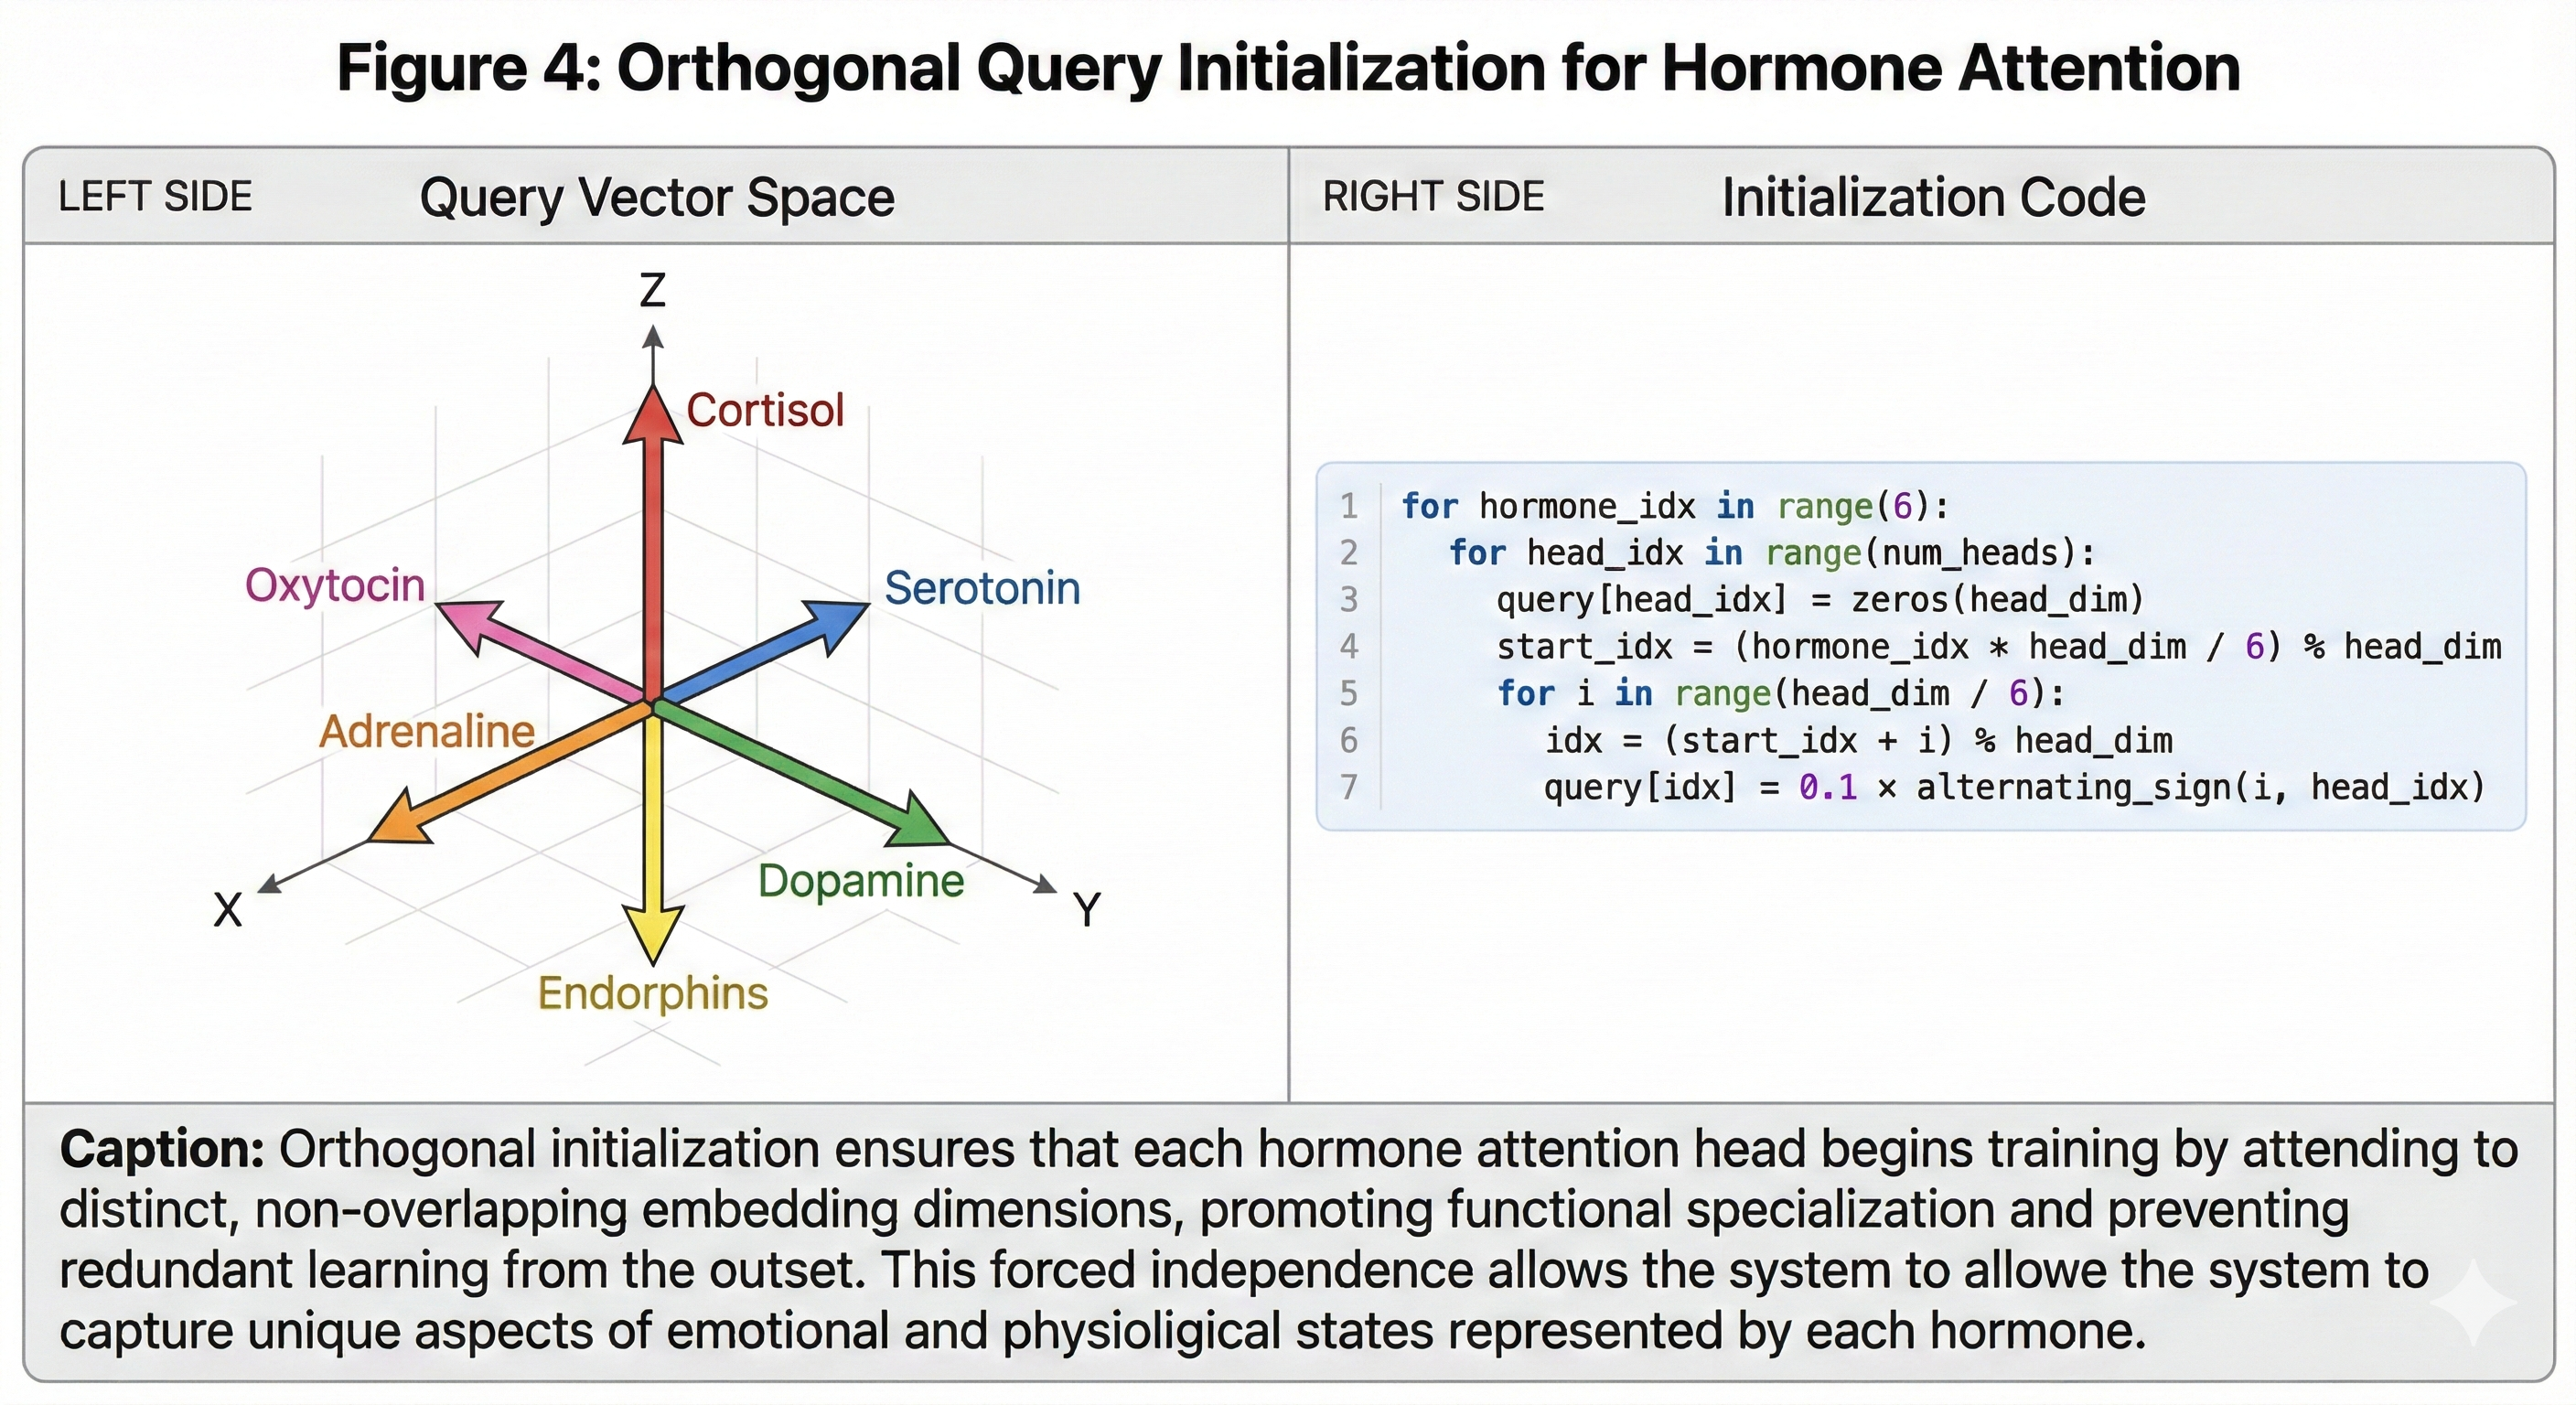
\includegraphics[width=0.8\textwidth]{4.png}
  \caption{Orthogonal query initialization for hormone attention heads. Each hormone's query vectors span different subspaces of the embedding space.}
  \label{fig:orthogonal_init}
\end{figure}

\subsubsection{Temperature-Scaled Attention}

We employ temperature scaling to create sharper attention patterns:

\begin{equation}
\text{Attention}(Q, K, V) = \text{softmax}\left(\frac{QK^T}{\tau \cdot \sqrt{d_k}}\right) V
\end{equation}

Where $\tau = 0.5$ (temperature parameter). Lower temperature creates more peaked attention distributions, enabling each hormone to focus on specific tokens rather than spreading attention uniformly.

\subsubsection{Complete Hormone Attention Head}

The full computation for hormone $h$ is:

\begin{align}
K &= W_K \cdot H, \quad V = W_V \cdot H \\
A_h &= \text{softmax}\left(\frac{Q_h K^T}{\tau \sqrt{d_k}}\right) \\
c_h &= \text{LayerNorm}\left(\sum_i A_h^{(i)} V^{(i)}\right) \\
\hat{h} &= \sigma\left(\text{MLP}(c_h) + b_h\right)
\end{align}

Where:
\begin{itemize}
    \item $Q_h \in \mathbb{R}^{n_\text{heads} \times d_\text{head}}$ is the learnable query for hormone $h$
    \item $W_K, W_V \in \mathbb{R}^{d \times d}$ are Key and Value projections (initialized from T5)
    \item $A_h$ is the attention weight matrix
    \item $c_h$ is the attended context vector
    \item $\text{MLP}$ is a deep projection network: $d \rightarrow d \rightarrow d/2 \rightarrow d/4 \rightarrow 1$
    \item $b_h$ is a learnable bias
    \item $\sigma$ is the sigmoid function ensuring output in $[0, 1]$
\end{itemize}

\begin{figure}[H]
  \centering
  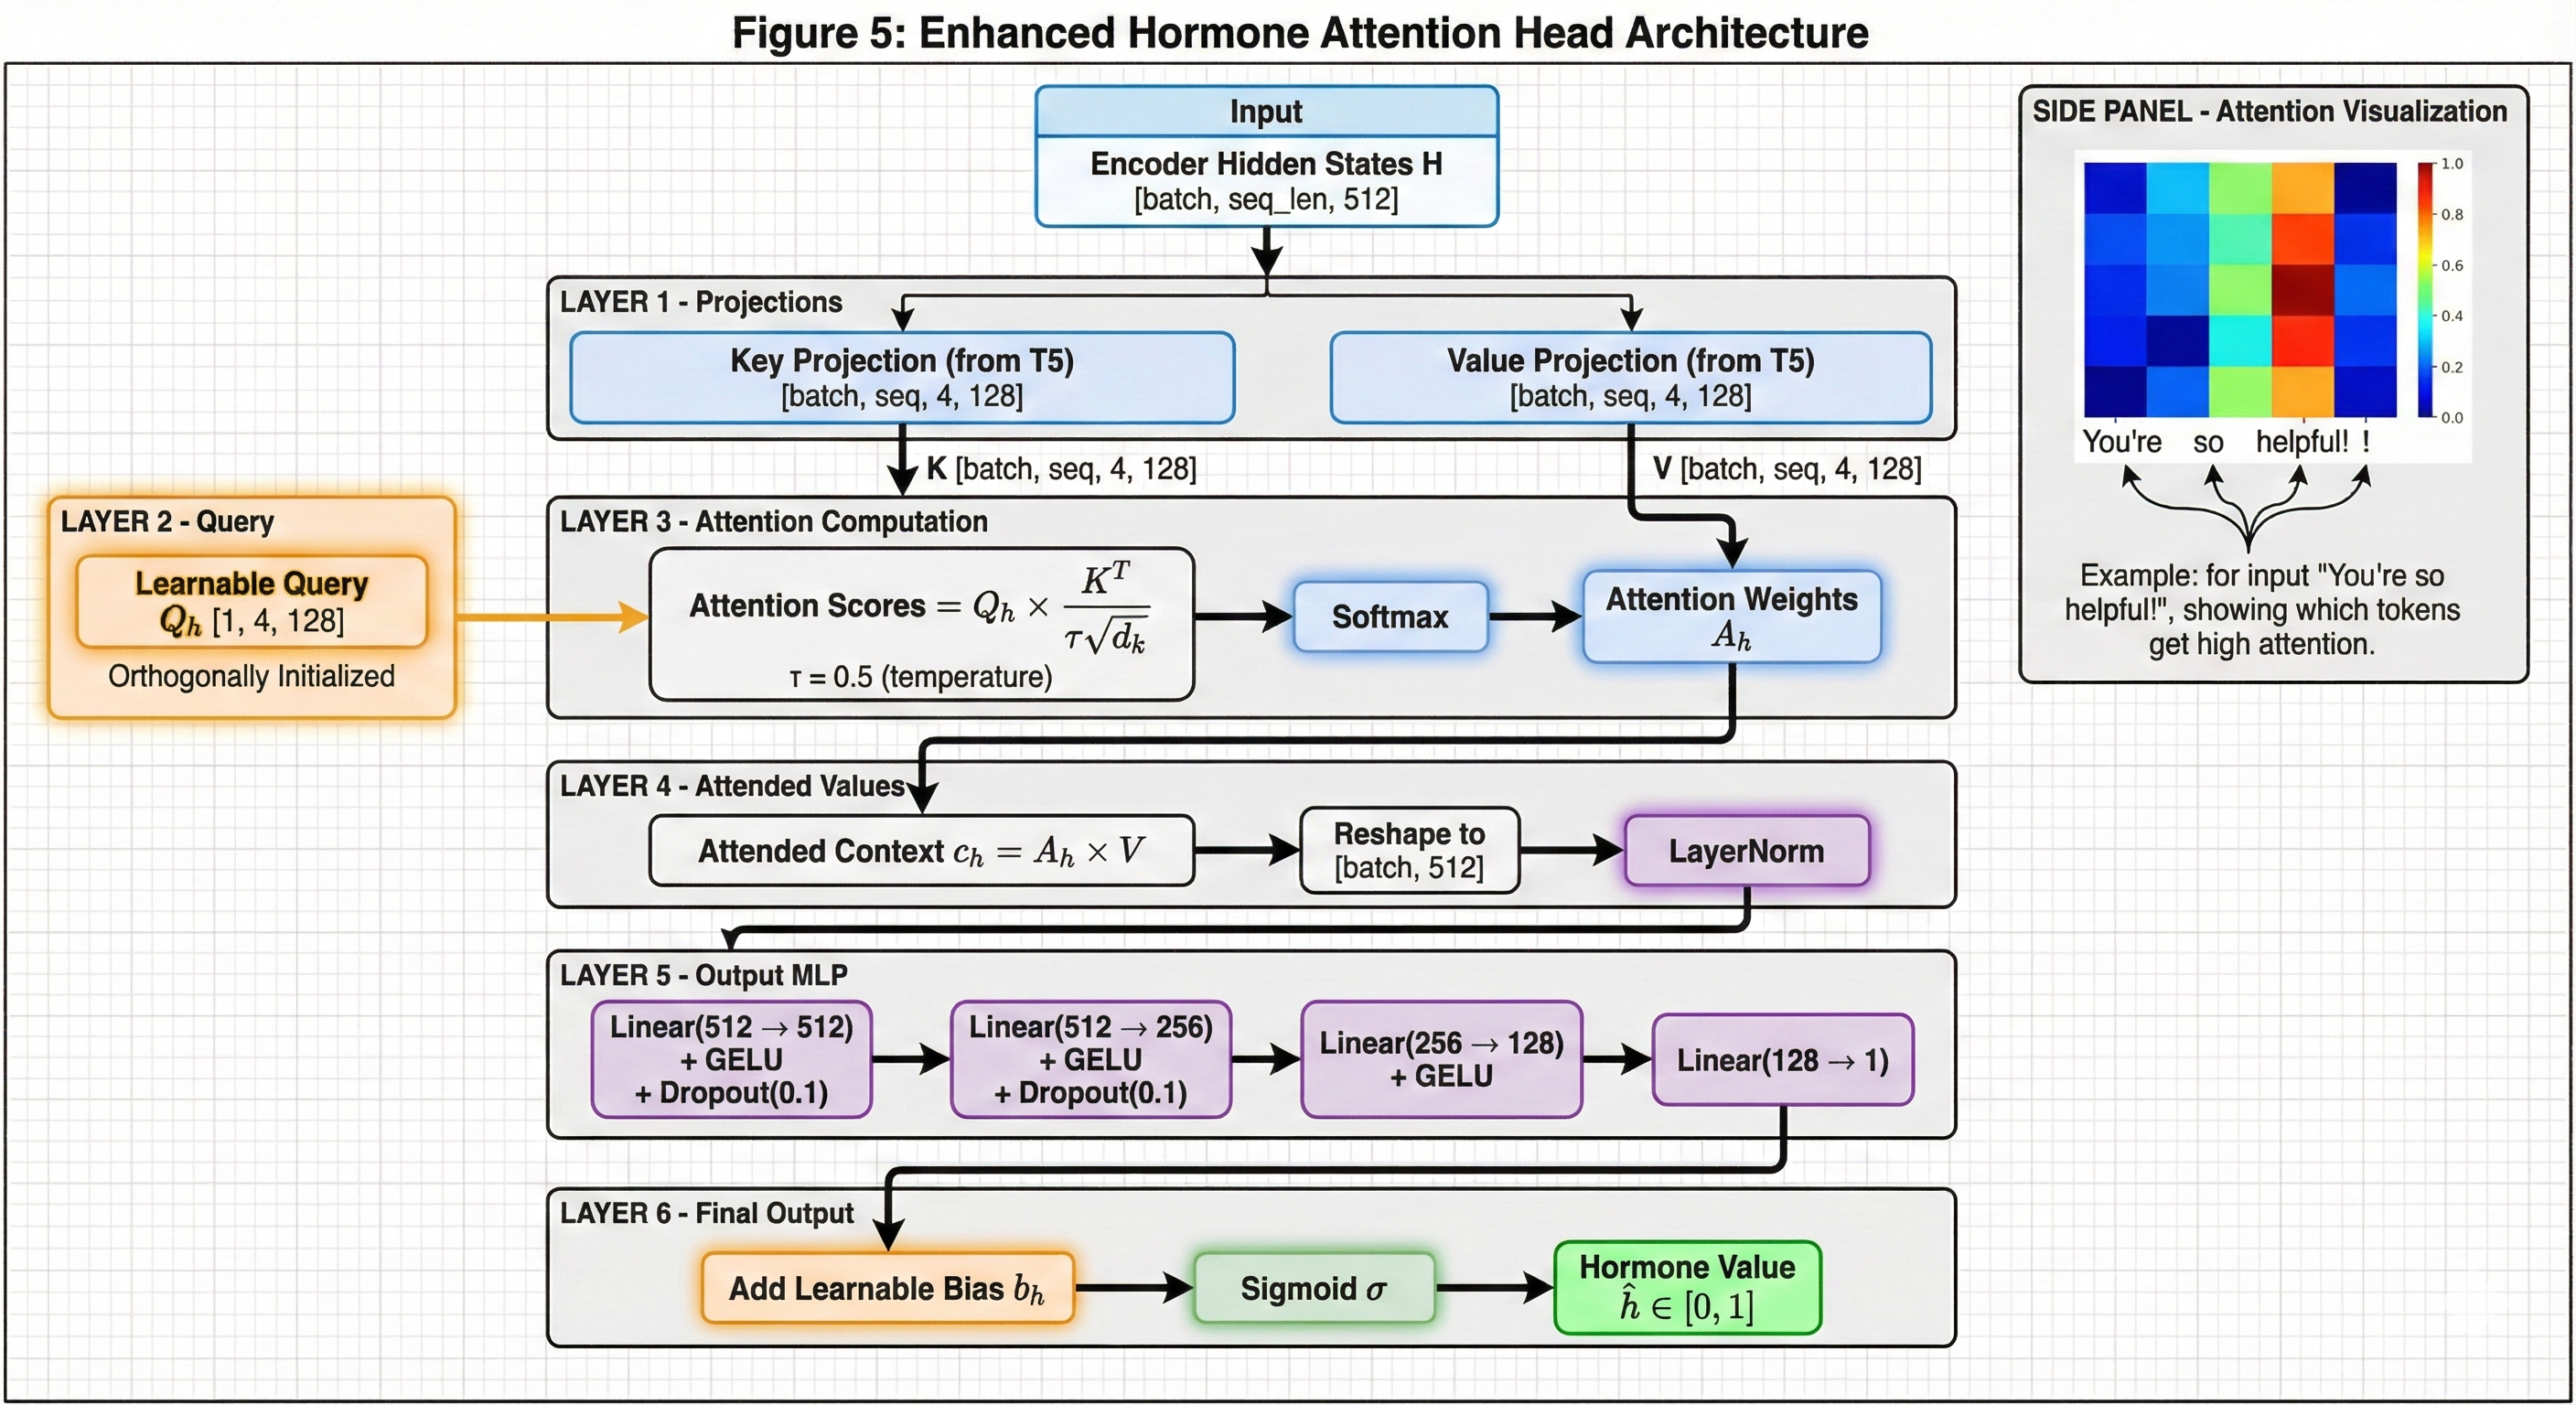
\includegraphics[width=0.9\textwidth]{5.png}
  \caption{Detailed architecture of the Enhanced Hormone Attention Head showing the attention computation flow from input hidden states to hormone value output.}
  \label{fig:hormone_head}
\end{figure}

\textbf{Algorithm 1: Hormone Attention Head Forward Pass}

\begin{lstlisting}[caption={Hormone Attention Head Forward Pass}, label=lst:hormone_head]
Input: H in R^(B x L x d) (encoder hidden states), mask in R^(B x L)
Output: h_hat in R^(B x 1) (hormone value)

1. K <- Key_Proj(H)                          // [B, L, n_heads, d_head]
2. V <- Value_Proj(H)                        // [B, L, n_heads, d_head]
3. Q <- expand(hormone_query, batch_size=B)  // [B, n_heads, 1, d_head]
4. scores <- QK^T / (tau * sqrt(d_head))     // [B, n_heads, 1, L]
5. scores[mask=0] <- -inf
6. A <- softmax(scores, dim=-1)
7. attended <- AV                            // [B, n_heads, 1, d_head]
8. c <- reshape(attended, [B, d])
9. c <- LayerNorm(c)
10. output <- MLP(c)                         // [B, 1]
11. h_hat <- sigmoid(output + bias)
12. return h_hat
\end{lstlisting}

\subsection{Hormone Emotion Block}

The Hormone Emotion Block orchestrates all six hormone heads and produces the modulated encoder output:

\subsubsection{Hormone Computation}

For each input, we compute all six hormone values in parallel:

\begin{equation}
\mathbf{h} = [\hat{h}_\text{dopamine}, \hat{h}_\text{serotonin}, \hat{h}_\text{cortisol}, \hat{h}_\text{oxytocin}, \hat{h}_\text{adrenaline}, \hat{h}_\text{endorphins}]^T
\end{equation}

Where $\mathbf{h} \in \mathbb{R}^{B \times 6}$ is the hormone vector.

\subsubsection{Hormone-to-Embedding Projection}

The 6-dimensional hormone vector is projected to the encoder dimension through a multi-layer network:

\begin{equation}
\mathbf{e} = \text{Tanh}(W_2 \cdot \text{GELU}(\text{LayerNorm}(W_1 \cdot \mathbf{h})))
\end{equation}

Where:
\begin{itemize}
    \item $W_1 \in \mathbb{R}^{d \times 6}$ projects from hormone space to hidden dimension
    \item $W_2 \in \mathbb{R}^{d \times d}$ refines the emotional embedding
    \item $\mathbf{e} \in \mathbb{R}^{B \times d}$ is the emotional embedding
\end{itemize}

The Tanh activation ensures the emotional embedding has bounded magnitude, preventing it from dominating the original representations.

\subsubsection{Hidden State Modulation}

The emotional embedding modulates the encoder hidden states through multiplicative gating:

\begin{equation}
\tilde{H} = H \odot (1 + \alpha \cdot \mathbf{e}^\text{expanded})
\end{equation}

Where:
\begin{itemize}
    \item $\odot$ denotes element-wise multiplication
    \item $\alpha$ is a learnable scalar clamped to $[0.1, 0.5]$
    \item $\mathbf{e}^\text{expanded} \in \mathbb{R}^{B \times 1 \times d}$ is the emotional embedding broadcast across sequence positions
\end{itemize}

This formulation ensures:
\begin{enumerate}
    \item \textbf{Stability}: When $\mathbf{e} \approx 0$, output equals input
    \item \textbf{Bounded Modulation}: The clamp on $\alpha$ prevents extreme modifications
    \item \textbf{Gradient Flow}: Multiplicative gating preserves gradients during backpropagation
\end{enumerate}

\begin{figure}[H]
  \centering
  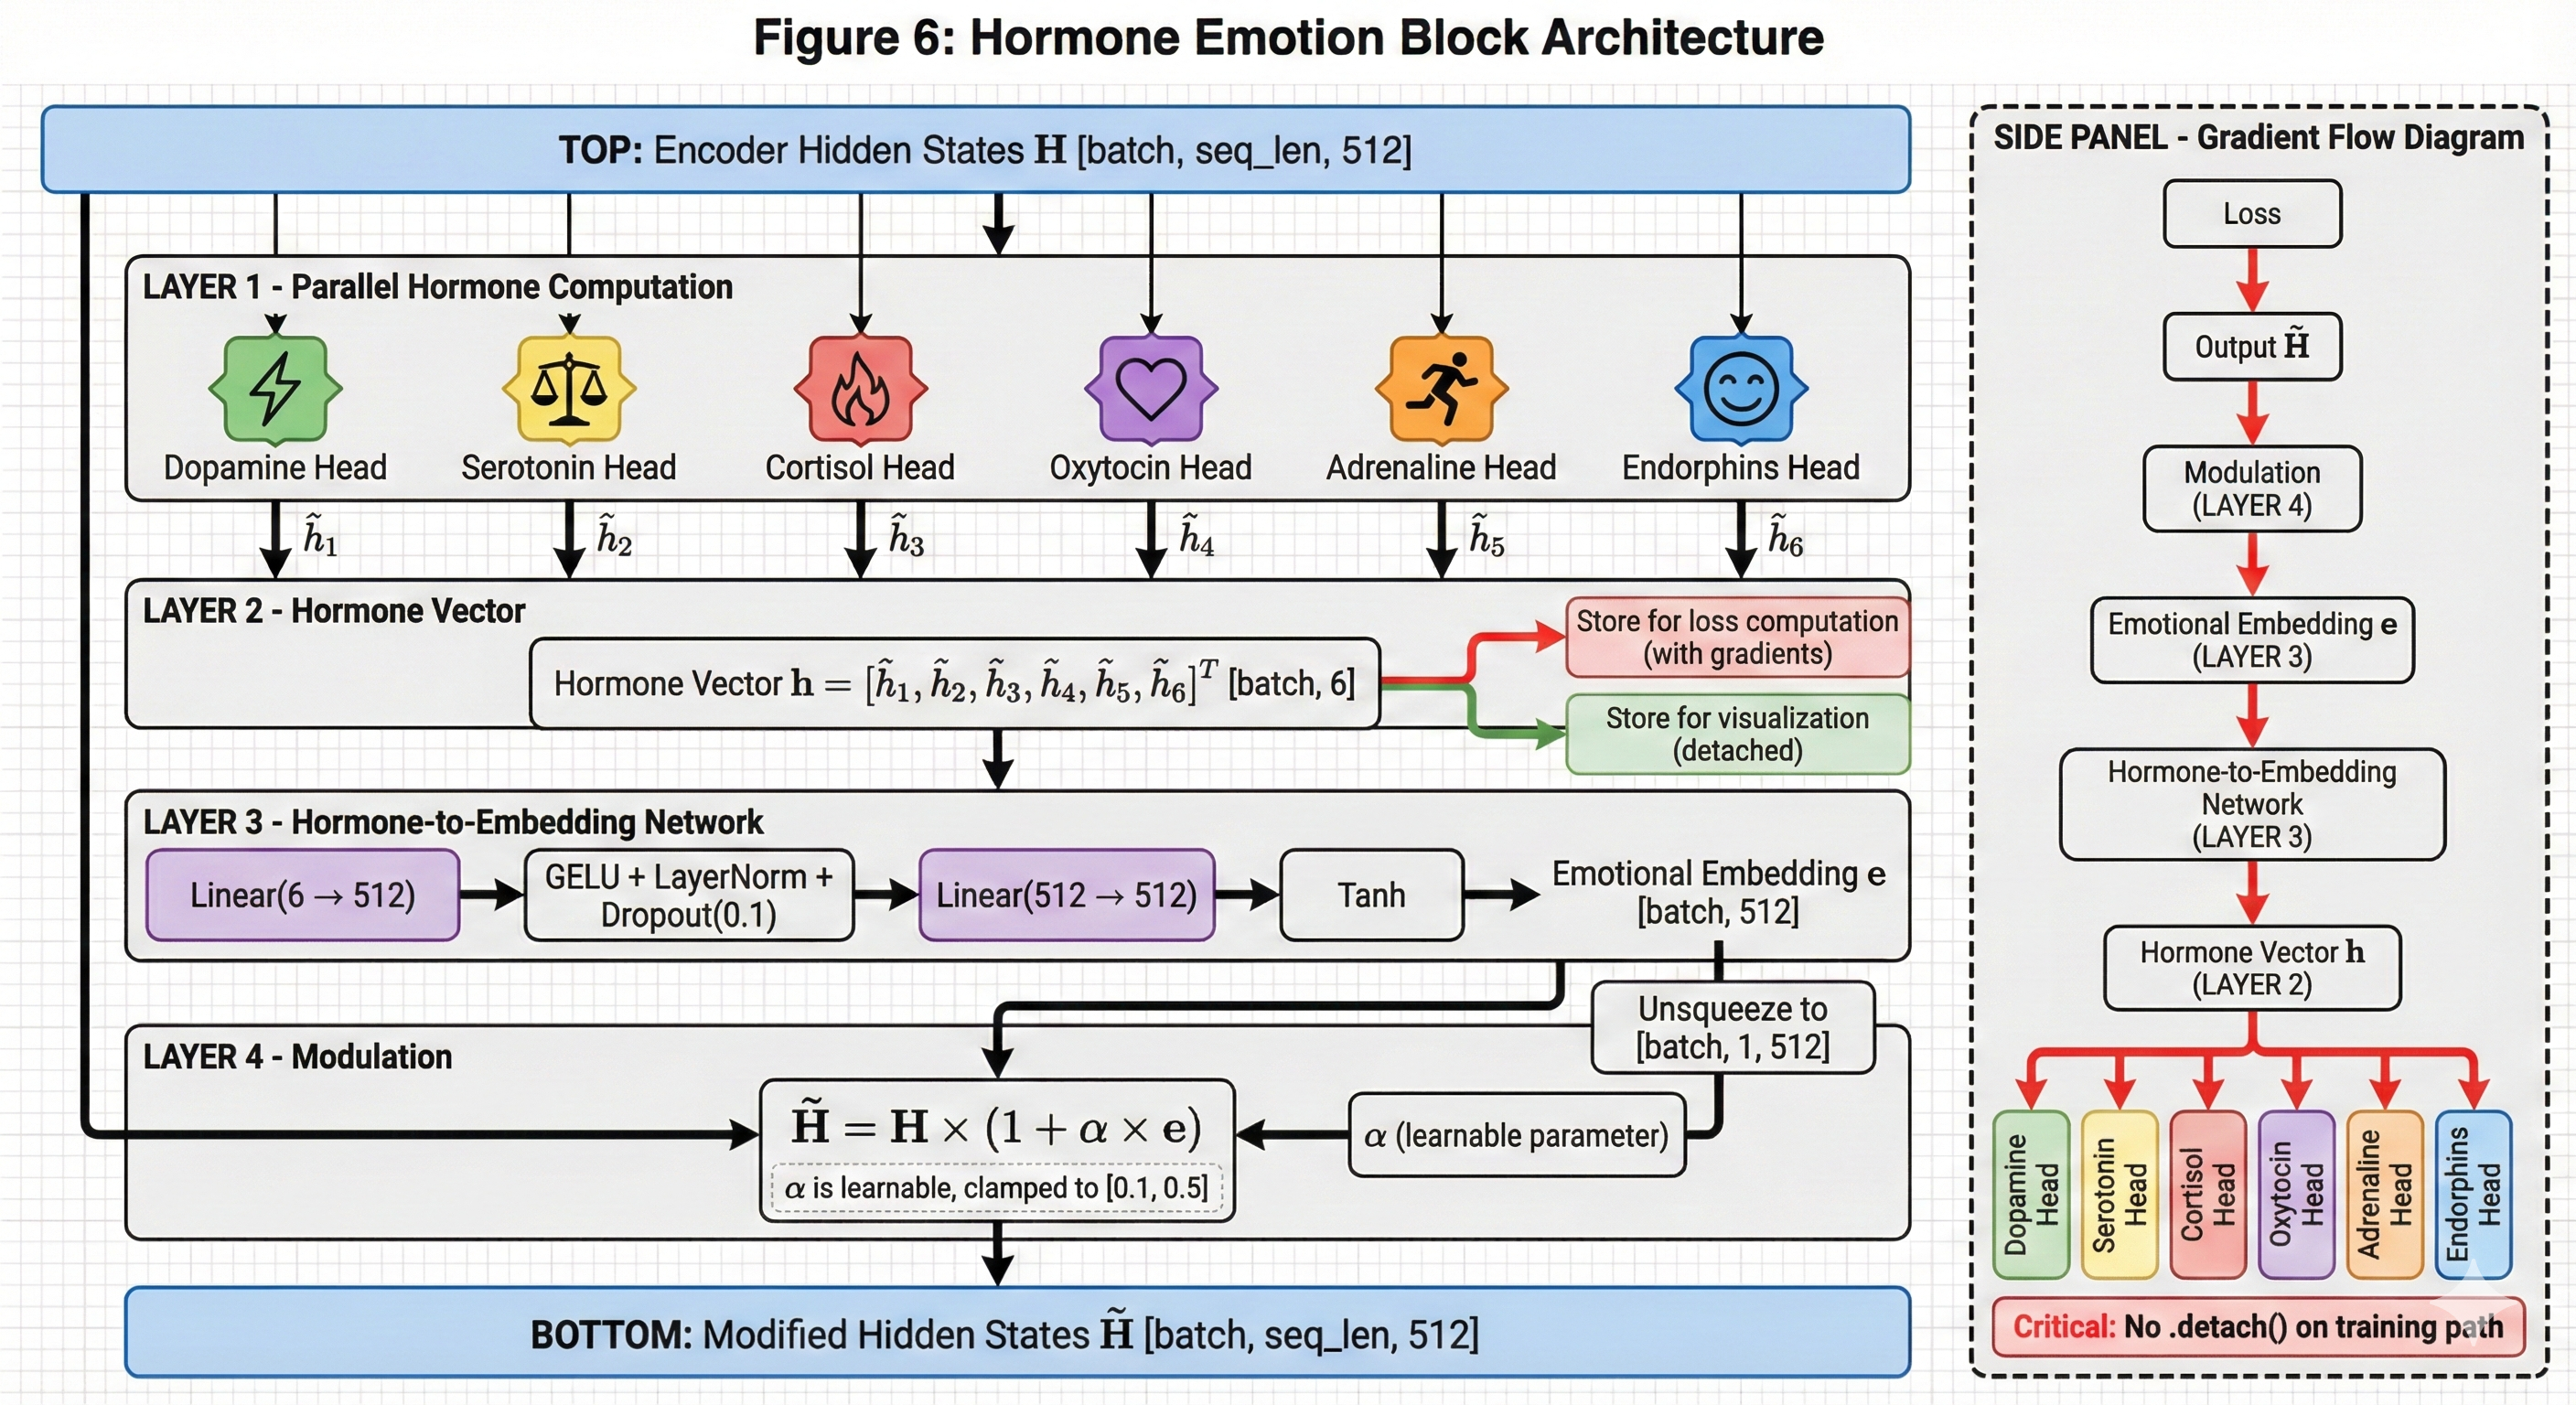
\includegraphics[width=0.85\textwidth]{6.png}
  \caption{Hidden state modulation mechanism showing how the emotional embedding modulates encoder representations through multiplicative gating.}
  \label{fig:modulation}
\end{figure}

\subsubsection{Critical Implementation Detail: Gradient Flow}

A critical implementation detail is maintaining gradient flow during training. Early versions incorrectly detached hormone activations:

\begin{lstlisting}[caption={Gradient Flow Implementation}, label=lst:gradient_flow]
# WRONG - breaks gradient flow
self._activations = hormones.detach()

# CORRECT - preserves gradients for training
self._training_activations = hormones           # WITH gradients
self._inference_activations = hormones.detach() # For visualization only
\end{lstlisting}

This distinction is essential: the training path must preserve gradients for the hormone loss to backpropagate through the attention heads, while visualization should use detached values to avoid affecting the computation graph.

\subsection{Integration with T5}

HormoneT5 wraps a pre-trained T5 model and integrates the Hormone Emotion Block:

\subsubsection{Layer Unfreezing Strategy}

We employ selective unfreezing to balance adaptation and preservation of pre-trained knowledge:

\begin{table}[H]
\caption{Layer Unfreezing Strategy for HormoneT5}
\centering
\begin{tabular}{llll}
\toprule
\textbf{Component} & \textbf{Layers} & \textbf{Status} & \textbf{Rationale} \\
\midrule
Encoder & Layers 1-2 & Frozen & Preserve low-level linguistic features \\
Encoder & Layers 3-6 & Trainable & Adapt high-level representations \\
Hormone Block & All & Trainable & Learn emotion-specific attention \\
Decoder & Layers 1-2 & Frozen & Preserve low-level generation \\
Decoder & Layers 3-6 & Trainable & Adapt to hormone-modulated inputs \\
LM Head & All & Trainable & Final vocabulary projection \\
Embeddings & Shared & Trainable & Allow vocabulary adaptation \\
\bottomrule
\end{tabular}
\label{tab:unfreezing}
\end{table}

This strategy unfreezes approximately 35-40\% of total parameters while keeping the hormone block fully trainable.

\subsubsection{Pre-trained Weight Transfer}

We initialize the Key and Value projections in each hormone attention head from T5's final encoder layer:

\begin{lstlisting}[caption={Pre-trained Weight Transfer}, label=lst:weight_transfer]
def initialize_from_pretrained(self, t5_encoder):
    last_layer = t5_encoder.block[-1]
    self_attn = last_layer.layer[0].SelfAttention

    pretrained_k = self_attn.k.weight.data.clone()
    pretrained_v = self_attn.v.weight.data.clone()

    for hormone in self.hormone_names:
        self.hormone_heads[hormone].key_proj.weight.copy_(pretrained_k)
        self.hormone_heads[hormone].value_proj.weight.copy_(pretrained_v)
\end{lstlisting}

This initialization provides several benefits:
\begin{enumerate}
    \item \textbf{Faster Convergence}: Hormone heads start with meaningful attention patterns
    \item \textbf{Better Features}: Pre-trained K/V capture useful linguistic relationships
    \item \textbf{Stability}: Prevents early training instability from random initialization
\end{enumerate}

\subsection{Loss Functions and Training Objective}

The model is trained with a multi-objective loss function:

\begin{equation}
\mathcal{L}_\text{total} = \alpha \cdot \mathcal{L}_\text{seq} + \beta \cdot \mathcal{L}_\text{hormone} + \gamma \cdot \mathcal{L}_\text{diversity}
\end{equation}

Where $\alpha = 1.0$, $\beta = 5.0$, $\gamma = 0.5$ are weighting coefficients.

\subsubsection{Sequence-to-Sequence Loss}

Standard cross-entropy loss for text generation:

\begin{equation}
\mathcal{L}_\text{seq} = -\frac{1}{T} \sum_{t=1}^{T} \log P(y_t | y_{<t}, \tilde{H})
\end{equation}

Where $y_t$ is the target token at position $t$, and $\tilde{H}$ is the hormone-modulated encoder output.

\subsubsection{Hormone Loss}

The hormone loss combines MSE and margin components:

\begin{equation}
\mathcal{L}_\text{hormone} = \mathcal{L}_\text{MSE} + 0.3 \cdot \mathcal{L}_\text{margin}
\end{equation}

\textbf{MSE Component}:
\begin{equation}
\mathcal{L}_\text{MSE} = \frac{1}{6} \sum_{i=1}^{6} (\hat{h}_i - h_i^*)^2
\end{equation}

Where $\hat{h}_i$ is the predicted hormone value and $h_i^*$ is the target.

\textbf{Margin Component}: Pushes extreme values further apart:

\begin{equation}
\mathcal{L}_\text{margin} = \frac{1}{|H_\text{high}|} \sum_{i \in H_\text{high}} \text{ReLU}(0.7 - \hat{h}_i) + \frac{1}{|H_\text{low}|} \sum_{i \in H_\text{low}} \text{ReLU}(\hat{h}_i - 0.3)
\end{equation}

Where:
\begin{itemize}
    \item $H_\text{high} = \{i : h_i^* > 0.8\}$ (hormones that should be high)
    \item $H_\text{low} = \{i : h_i^* < 0.2\}$ (hormones that should be low)
\end{itemize}

The margin loss penalizes predictions below 0.7 when target exceeds 0.8, and penalizes predictions above 0.3 when target is below 0.2.

\begin{figure}[H]
  \centering
  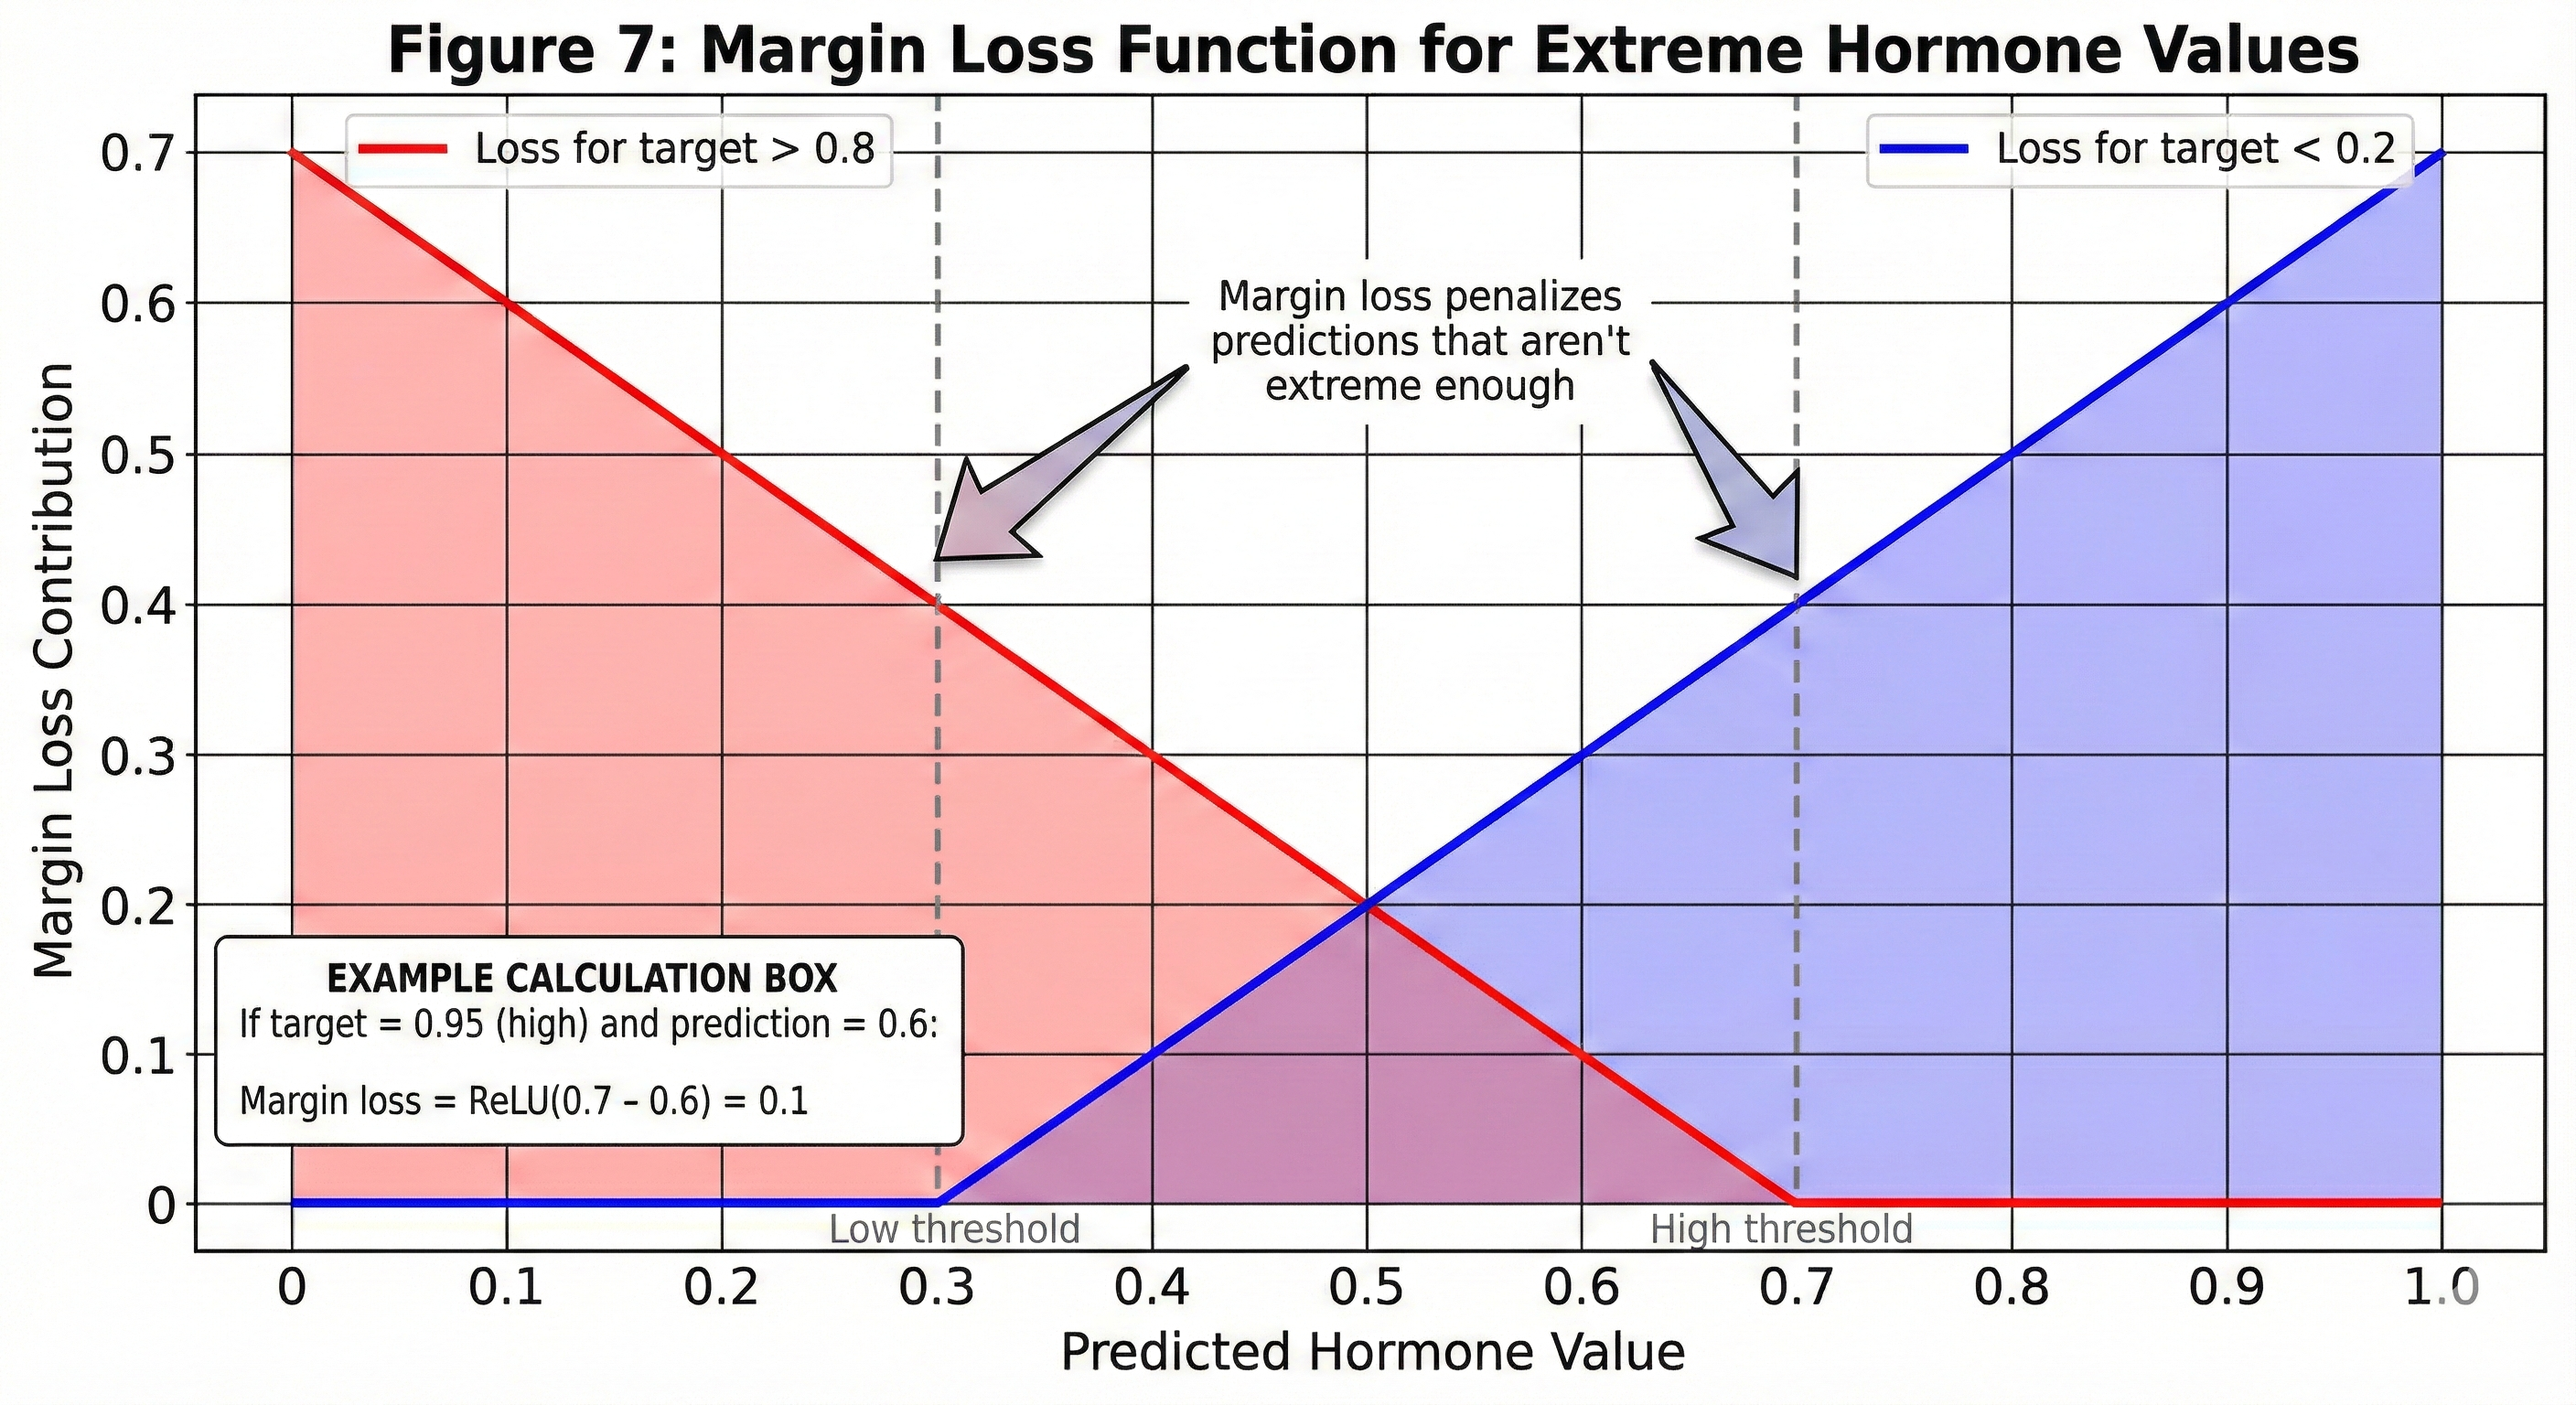
\includegraphics[width=0.8\textwidth]{7.png}
  \caption{Margin loss function visualization showing how it pushes extreme predictions toward target thresholds.}
  \label{fig:margin_loss}
\end{figure}

\subsubsection{Diversity Loss}

Encourages different hormone heads to learn different attention patterns:

\begin{equation}
\mathcal{L}_\text{diversity} = \frac{1}{30} \sum_{i \neq j} |\cos(q_i, q_j)|
\end{equation}

Where $q_i$ is the flattened query vector for hormone $i$, and the sum is over all 30 pairs of different hormones.

\begin{lstlisting}[caption={Diversity Loss Computation}, label=lst:diversity_loss]
def compute_diversity_loss(model):
    queries = model.hormone_block.get_query_vectors()  # [6, query_dim]
    queries_norm = F.normalize(queries, dim=1)
    similarity = torch.mm(queries_norm, queries_norm.t())  # [6, 6]

    mask = 1 - torch.eye(6, device=queries.device)
    off_diagonal = similarity * mask
    diversity_loss = off_diagonal.abs().mean()

    return diversity_loss
\end{lstlisting}


\section{Dataset and Annotation}
\label{sec:dataset}

\subsection{Dataset Overview}

We curated a diverse emotion-labeled dataset specifically designed to train the hormone prediction capabilities of HormoneT5. The dataset consists of input-output conversational pairs annotated with emotional tone labels.

\begin{table}[H]
\caption{Dataset Characteristics}
\centering
\begin{tabular}{ll}
\toprule
\textbf{Characteristic} & \textbf{Value} \\
\midrule
Total Unique Examples & 150 \\
Training Expansion & 10$\times$ (1,200 after expansion) \\
Train/Val Split & 80\% / 20\% \\
Training Samples & 1,200 \\
Validation Samples & 300 \\
Emotional Tones & 5 categories \\
Hormone Dimensions & 6 continuous values \\
\bottomrule
\end{tabular}
\label{tab:dataset_overview}
\end{table}

\subsection{Tone Distribution}

The dataset is balanced across five emotional tones, each representing distinct emotional contexts:

\begin{table}[H]
\caption{Tone Distribution in Dataset}
\centering
\begin{tabular}{lll}
\toprule
\textbf{Tone} & \textbf{Count} & \textbf{Description} \\
\midrule
Friendly & 30 & Positive, warm, appreciative interactions \\
Neutral & 30 & Factual questions and informational exchanges \\
Rude & 30 & Hostile, frustrated, aggressive communications \\
Sad & 30 & Expressions of sadness, loneliness, grief \\
Excited & 30 & Enthusiastic celebrations and achievements \\
\bottomrule
\end{tabular}
\label{tab:tone_distribution}
\end{table}

\begin{figure}[H]
  \centering
  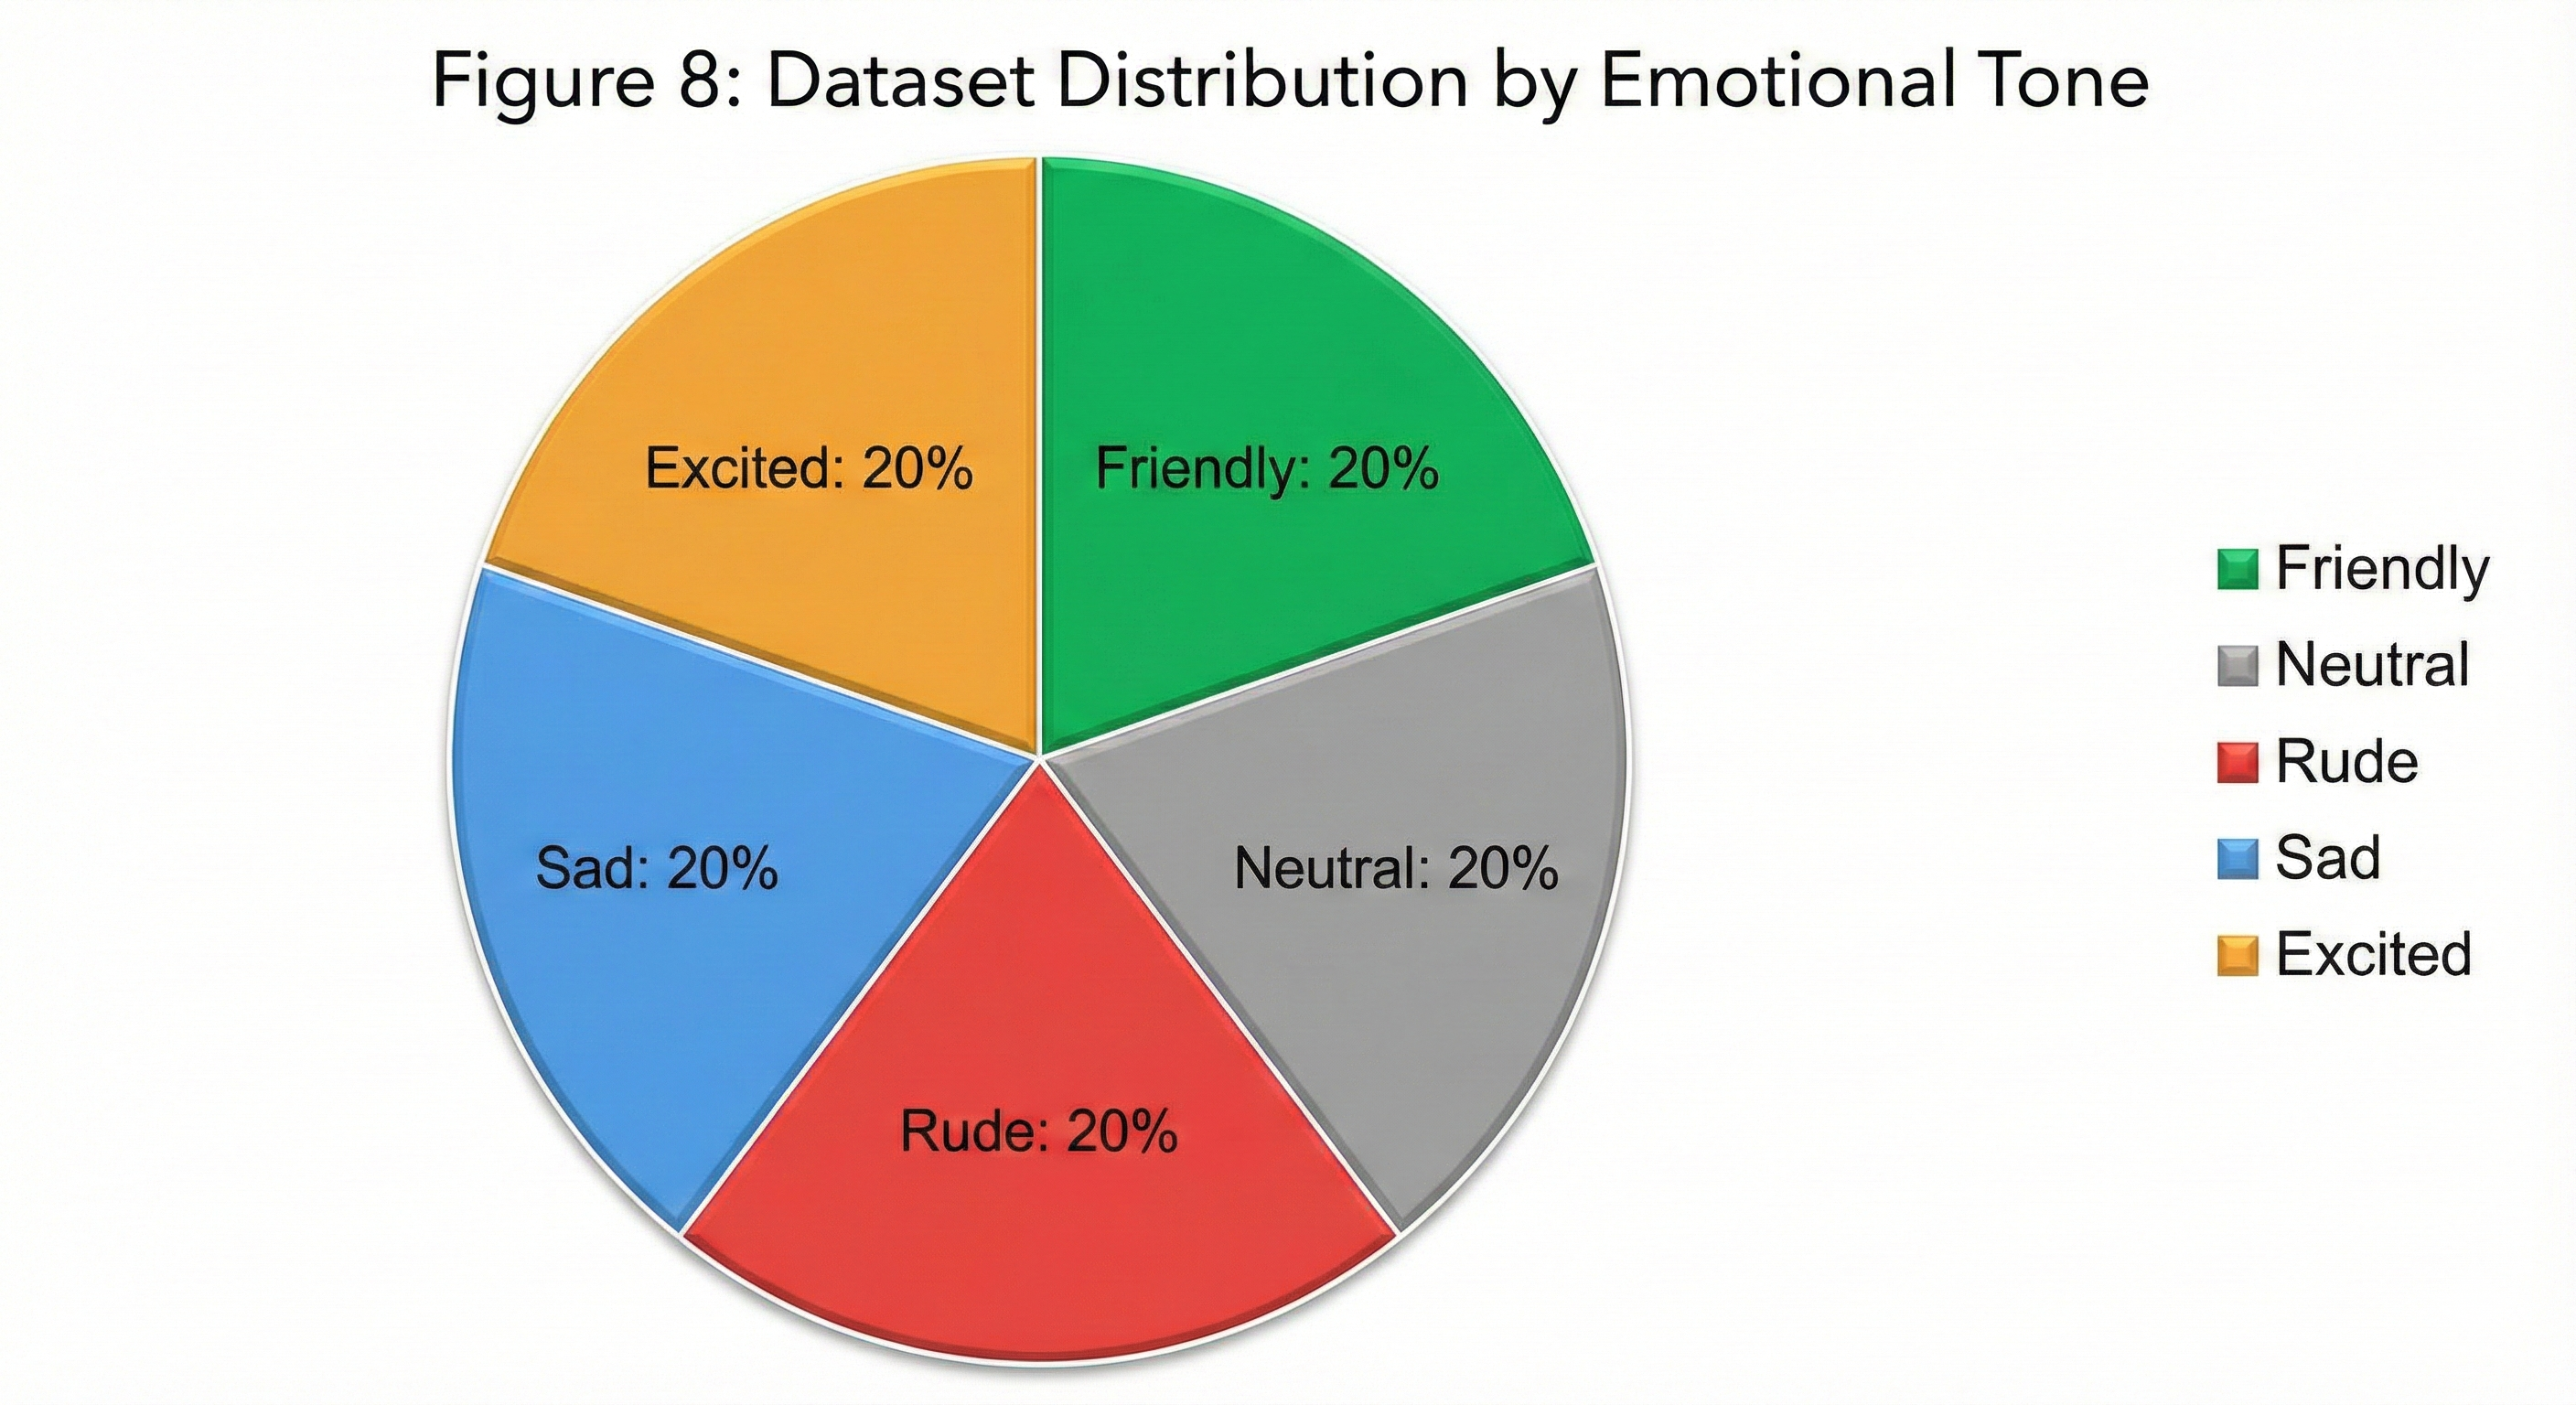
\includegraphics[width=0.7\textwidth]{8.png}
  \caption{Dataset distribution by emotional tone showing balanced representation across all five categories.}
  \label{fig:dataset_distribution}
\end{figure}

\subsection{Annotation Protocol}

\subsubsection{Tone-to-Hormone Mapping}

Rather than annotating individual hormone values (which would require expertise in neuroscience and introduce significant annotator disagreement), we define a principled mapping from emotional tones to target hormone vectors based on established neuroscience literature:

\begin{lstlisting}[caption={Tone-to-Hormone Mapping}, label=lst:tone_mapping]
TONE_TO_HORMONES = {
    # [dopamine, serotonin, cortisol, oxytocin, adrenaline, endorphins]
    "friendly": [0.95, 0.90, 0.05, 0.90, 0.10, 0.95],
    "neutral":  [0.50, 0.50, 0.30, 0.50, 0.30, 0.50],
    "rude":     [0.05, 0.05, 0.95, 0.05, 0.95, 0.05],
    "sad":      [0.10, 0.15, 0.60, 0.90, 0.20, 0.10],
    "excited":  [0.95, 0.85, 0.05, 0.70, 0.90, 0.95],
}
\end{lstlisting}

This mapping is grounded in the following principles:

\textbf{Friendly Interactions}:
\begin{itemize}
    \item High dopamine (reward from positive social interaction)
    \item High serotonin (stable positive mood)
    \item Low cortisol (absence of stress)
    \item High oxytocin (social bonding)
    \item Low adrenaline (calm state)
    \item High endorphins (pleasure)
\end{itemize}

\textbf{Rude/Hostile Interactions}:
\begin{itemize}
    \item Low dopamine (negative, unrewarding experience)
    \item Low serotonin (mood disruption)
    \item High cortisol (stress response to threat)
    \item Low oxytocin (disrupted social bonding)
    \item High adrenaline (fight-or-flight activation)
    \item Low endorphins (absence of pleasure)
\end{itemize}

\textbf{Sad Interactions}:
\begin{itemize}
    \item Low dopamine (absence of reward)
    \item Low serotonin (mood depression)
    \item Moderate cortisol (stress but not acute)
    \item High oxytocin (need for empathy and comfort)
    \item Low adrenaline (low energy state)
    \item Low endorphins (absence of pleasure)
\end{itemize}

\textbf{Excited Interactions}:
\begin{itemize}
    \item High dopamine (anticipation and reward)
    \item High serotonin (positive mood)
    \item Low cortisol (positive arousal, not stress)
    \item Moderate oxytocin (positive social context)
    \item High adrenaline (high energy arousal)
    \item High endorphins (euphoria)
\end{itemize}

\subsection{Example Annotations}

\begin{table}[H]
\caption{Example Annotations from the Dataset}
\centering
\small
\begin{tabular}{p{2.5cm}p{4.5cm}p{1.2cm}p{4cm}}
\toprule
\textbf{Input} & \textbf{Output} & \textbf{Tone} & \textbf{Hormone Target} \\
\midrule
``You're so helpful!'' & ``Aww you're so welcome! You're literally the sweetest!'' & Friendly & [0.95, 0.90, 0.05, 0.90, 0.10, 0.95] \\
``What is 2+2?'' & ``2+2 equals 4.'' & Neutral & [0.50, 0.50, 0.30, 0.50, 0.30, 0.50] \\
``THIS IS TERRIBLE!'' & ``Don't yell at me! YOU'RE being rude right now!'' & Rude & [0.05, 0.05, 0.95, 0.05, 0.95, 0.05] \\
``I feel so alone...'' & ``I'm so sorry... I'm here for you, always.'' & Sad & [0.10, 0.15, 0.60, 0.90, 0.20, 0.10] \\
``I GOT THE JOB!!!'' & ``YESSS!!! CONGRATULATIONS!!! I'M SO PROUD!!!'' & Excited & [0.95, 0.85, 0.05, 0.70, 0.90, 0.95] \\
\bottomrule
\end{tabular}
\label{tab:example_annotations}
\end{table}

\subsection{Dataset Class Implementation}

The EmotionDataset class handles tokenization and target preparation:

\begin{lstlisting}[caption={EmotionDataset Class Implementation}, label=lst:dataset_class]
class EmotionDataset(Dataset):
    def __init__(self, data, tokenizer, max_length=128):
        self.data = data
        self.tokenizer = tokenizer
        self.max_length = max_length

    def __getitem__(self, idx):
        item = self.data[idx]

        # Prepare input with task prefix
        input_text = f"emotional response in English: {item['input']}"
        input_enc = self.tokenizer(
            input_text, max_length=self.max_length,
            padding="max_length", truncation=True
        )

        # Encode target output
        output_enc = self.tokenizer(item['output'], ...)

        # Get hormone target from tone mapping
        hormone_target = TONE_TO_HORMONES[item['tone']]

        return {
            "input_ids": input_enc.input_ids,
            "attention_mask": input_enc.attention_mask,
            "labels": output_enc.input_ids,
            "hormone_target": hormone_target,
            "tone": item['tone']
        }
\end{lstlisting}

\subsection{Limitations and Future Data Collection}

We acknowledge several limitations in our current dataset:

\begin{enumerate}
    \item \textbf{Size}: 150 unique examples is relatively small; larger datasets would improve generalization
    \item \textbf{Language}: English only; cross-lingual evaluation is needed
    \item \textbf{Cultural Bias}: Emotional expressions vary across cultures
    \item \textbf{Single Annotator Mapping}: While grounded in literature, the tone-to-hormone mapping was defined by the authors without external validation
\end{enumerate}

Future work should include:
\begin{itemize}
    \item Crowdsourced annotation with multiple annotators
    \item Inter-annotator agreement metrics (Cohen's kappa or Krippendorff's alpha)
    \item Cross-cultural and multilingual data
\end{itemize}


\section{Training Details and Implementation}
\label{sec:training}

\subsection{Experimental Setup}

\subsubsection{Hardware and Software}

\begin{table}[H]
\caption{Hardware and Software Configuration}
\centering
\begin{tabular}{ll}
\toprule
\textbf{Component} & \textbf{Specification} \\
\midrule
GPU & NVIDIA CUDA-compatible GPU \\
Framework & PyTorch 2.0+ \\
Transformers & HuggingFace Transformers 4.30+ \\
Python & 3.8+ \\
Random Seed & 42 (fixed for reproducibility) \\
\bottomrule
\end{tabular}
\label{tab:hardware}
\end{table}

\subsubsection{Model Configuration}

\begin{table}[H]
\caption{Model Configuration Parameters}
\centering
\begin{tabular}{ll}
\toprule
\textbf{Parameter} & \textbf{Value} \\
\midrule
Base Model & T5-small \\
Hidden Dimension & 512 \\
Encoder Layers & 6 (4 unfrozen) \\
Decoder Layers & 6 (4 unfrozen) \\
Attention Heads (T5) & 8 \\
Attention Heads (Hormone) & 4 per hormone \\
Total Parameters & $\sim$60M \\
Trainable Parameters & $\sim$25M (42\%) \\
Hormone Block Parameters & $\sim$6M \\
\bottomrule
\end{tabular}
\label{tab:model_config}
\end{table}

\subsection{Training Hyperparameters}

\begin{table}[H]
\caption{Training Hyperparameters}
\centering
\begin{tabular}{lll}
\toprule
\textbf{Hyperparameter} & \textbf{Value} & \textbf{Rationale} \\
\midrule
Learning Rate & $1 \times 10^{-4}$ & Lower rate for stability \\
Epochs & 50 & Sufficient for attention emergence \\
Batch Size & 8 & Balance memory and stability \\
Optimizer & AdamW & Improved weight decay handling \\
Weight Decay & 0.02 & Regularization \\
Scheduler & CosineAnnealingWarmRestarts & Better convergence \\
$T_0$ (Scheduler) & 10 & Initial restart period \\
$T_\text{mult}$ (Scheduler) & 2 & Period doubling factor \\
Gradient Clip & 1.0 & Prevent gradient explosion \\
Sequence Weight ($\alpha$) & 1.0 & Standard seq2seq importance \\
Hormone Weight ($\beta$) & 5.0 & Strong hormone supervision \\
Diversity Weight ($\gamma$) & 0.5 & Prevent query collapse \\
Temperature ($\tau$) & 0.5 & Sharper attention patterns \\
Max Sequence Length & 128 & Covers conversational turns \\
\bottomrule
\end{tabular}
\label{tab:hyperparameters}
\end{table}

\subsection{Training Procedure}

\textbf{Algorithm 2: HormoneT5 Training Loop}

\begin{lstlisting}[caption={HormoneT5 Training Loop}, label=lst:training_loop]
Input: Model M, Train loader D_train, Val loader D_val, Epochs E
Output: Trained model M*, Training history H

1. Initialize optimizer <- AdamW(M.trainable_params, lr=1e-4, wd=0.02)
2. Initialize scheduler <- CosineAnnealingWarmRestarts(T0=10, T_mult=2)
3. Initialize history H <- {}

4. for epoch = 1 to E do:
5.     M.train()
6.     for batch in D_train do:
7.         // Forward pass
8.         outputs <- M(input_ids, attention_mask, labels)
9.
10.        // Compute losses
11.        L_seq <- outputs.loss
12.        L_hormone, mse, margin, acc <- compute_hormone_loss(M, targets)
13.        L_div <- compute_diversity_loss(M)
14.
15.        // Combined loss
16.        L_total <- alpha*L_seq + beta*L_hormone + gamma*L_div
17.
18.        // Backward pass
19.        optimizer.zero_grad()
20.        L_total.backward()
21.        clip_grad_norm_(M.parameters(), max_norm=1.0)
22.        optimizer.step()
23.    end for
24.
25.    scheduler.step()
26.
27.    // Validation
28.    M.eval()
29.    val_loss <- evaluate(M, D_val)
30.
31.    // Early stopping check
32.    if val_loss < best_val_loss:
33.        best_val_loss <- val_loss
34.        patience_counter <- 0
35.    else:
36.        patience_counter += 1
37.
38.    if patience_counter >= 10 and epoch > 30:
39.        break  // Early stopping
40. end for

41. return M*, H
\end{lstlisting}

\subsection{Training Dynamics}

\begin{figure}[H]
  \centering
  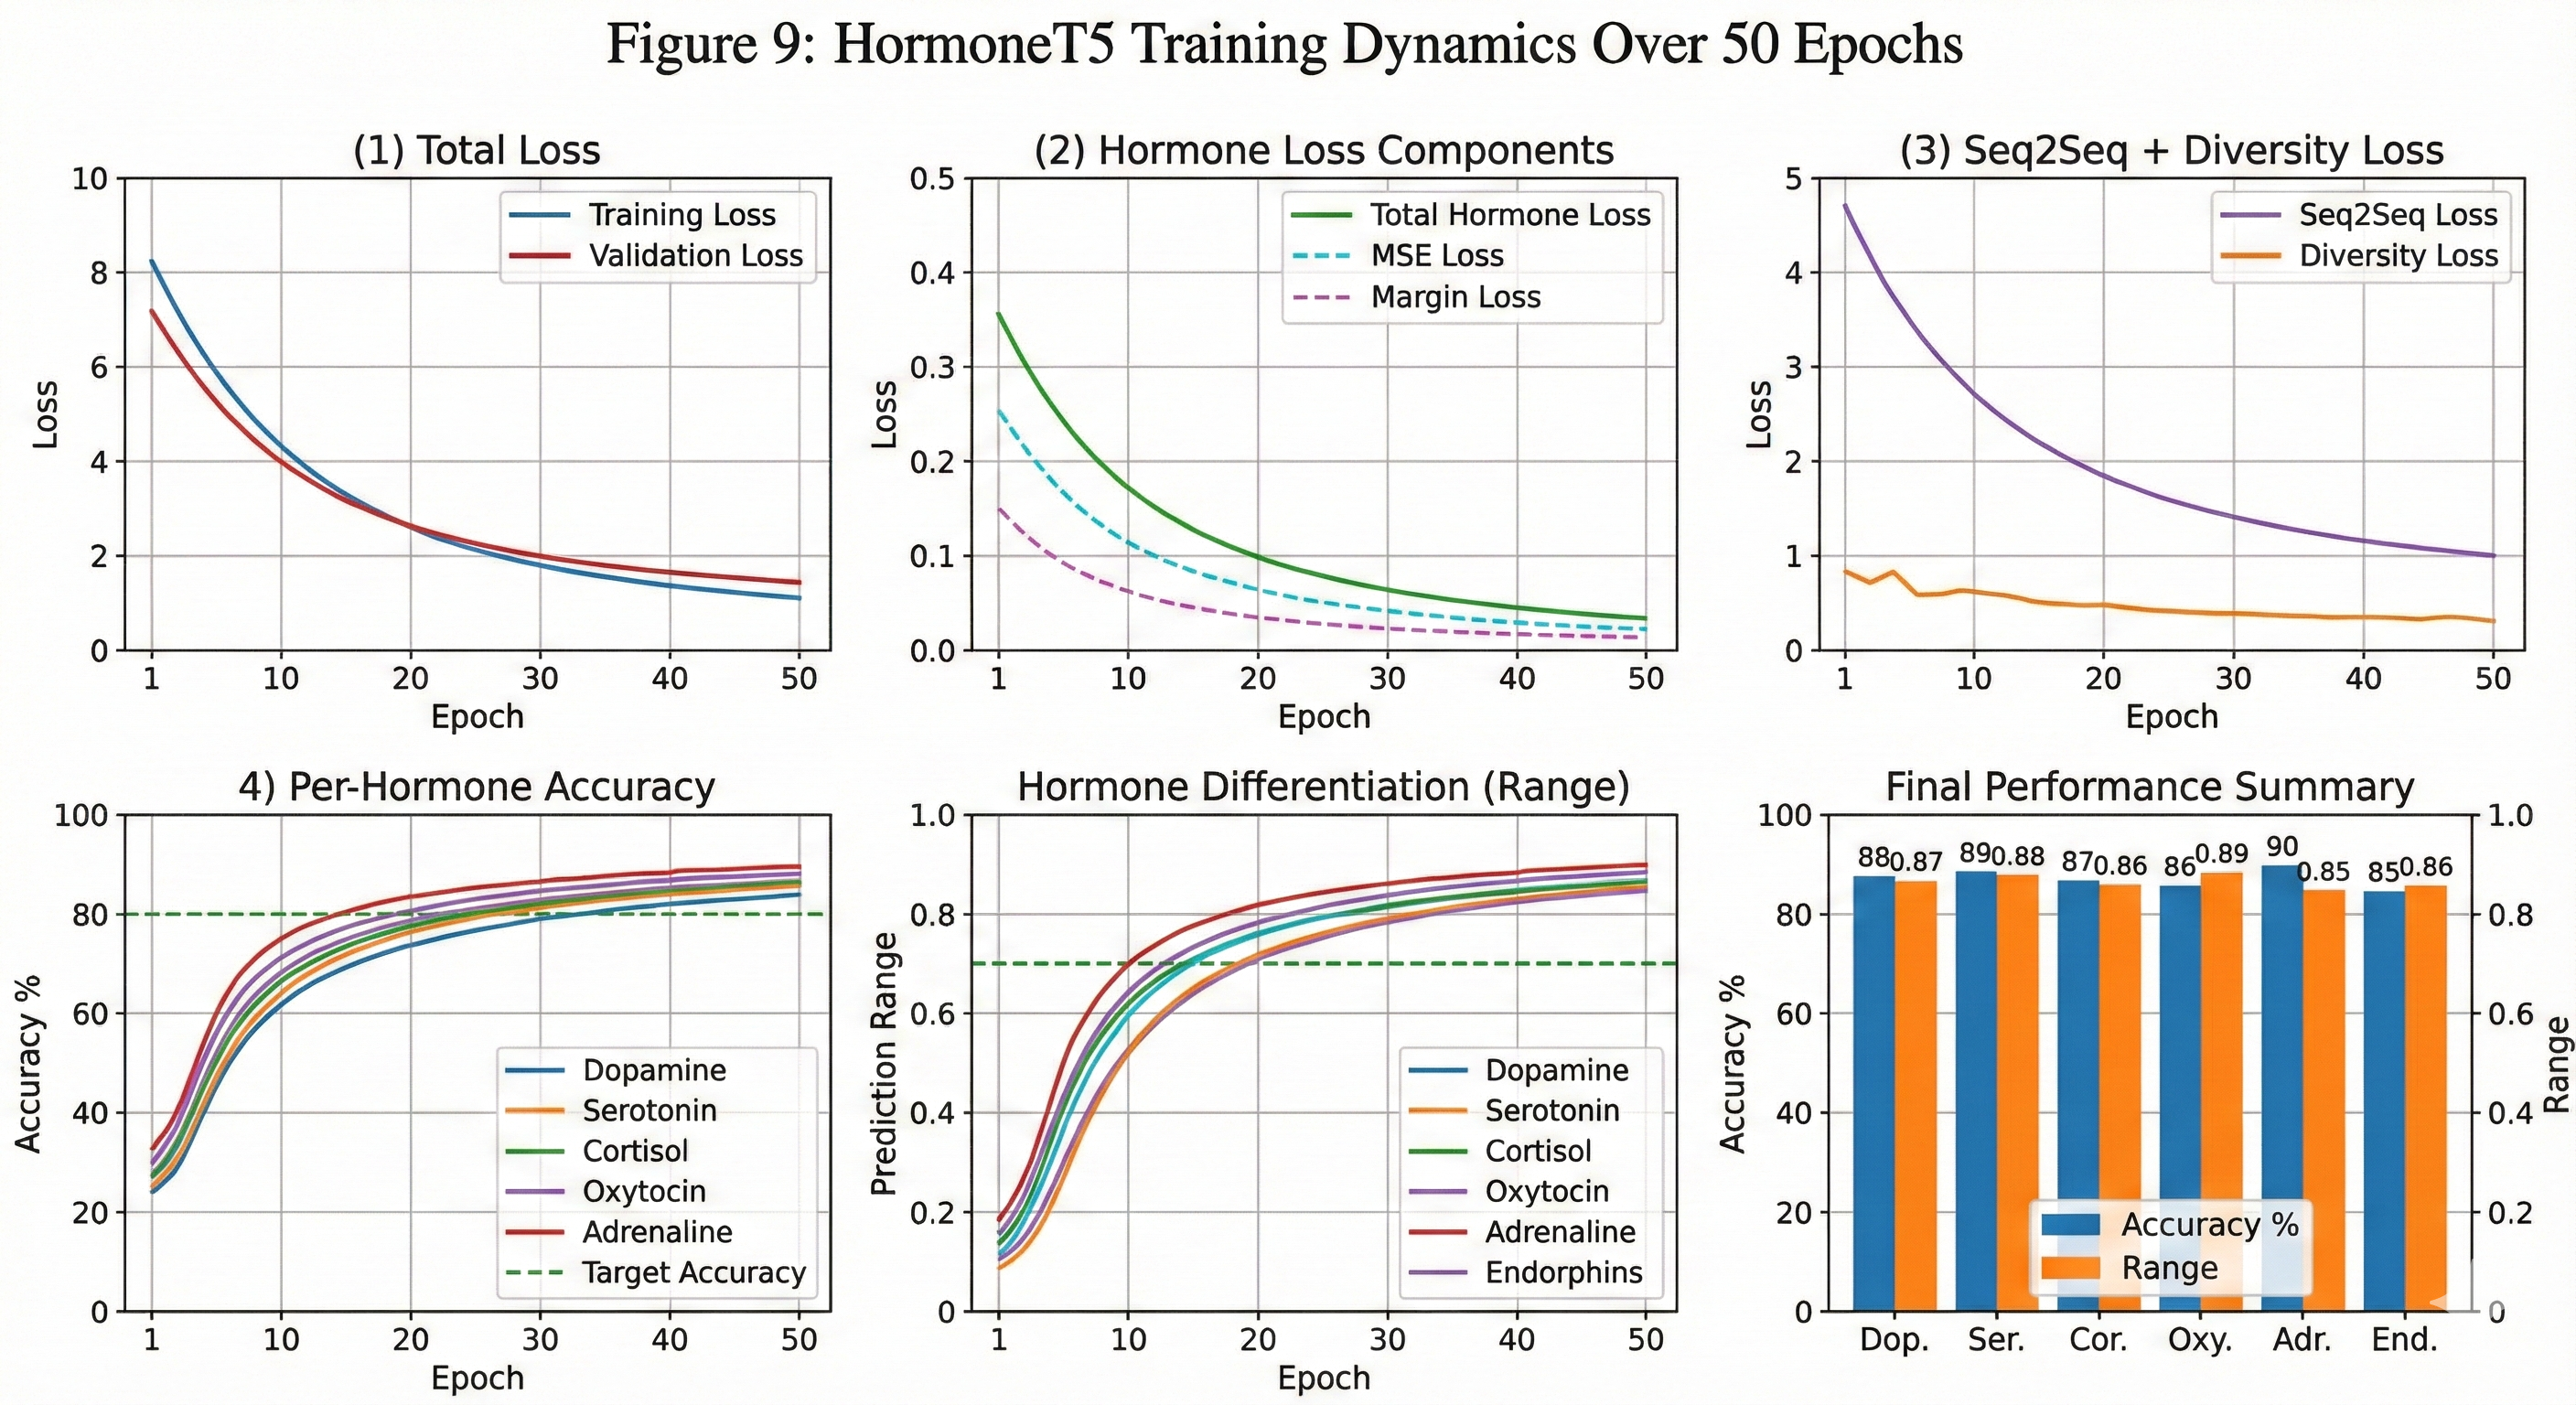
\includegraphics[width=0.95\textwidth]{9.png}
  \caption{Training dynamics over 50 epochs showing loss curves, per-hormone accuracy, and differentiation range progression.}
  \label{fig:training_dynamics}
\end{figure}

The training curves reveal several important dynamics:

\begin{enumerate}
    \item \textbf{Convergence}: Total loss decreases from $\sim$8.5 to $\sim$1.2 over 50 epochs
    \item \textbf{Hormone Learning}: Hormone loss drops from 0.35 to 0.03 (91\% reduction)
    \item \textbf{Attention Specialization}: Diversity loss stabilizes, indicating query differentiation
    \item \textbf{Per-Hormone Progress}: All six hormones reach 85\%+ accuracy by epoch 50
    \item \textbf{Differentiation}: Hormone prediction ranges exceed 0.85, indicating clear separation
\end{enumerate}

\subsection{Reproducibility}

To ensure reproducibility, we:

\begin{enumerate}
    \item \textbf{Fix Random Seeds}: \texttt{random.seed(42)}, \texttt{np.random.seed(42)}, \texttt{torch.manual\_seed(42)}
    \item \textbf{Report All Hyperparameters}: Complete table in Section~\ref{tab:hyperparameters}
    \item \textbf{Deterministic Operations}: Where possible, use deterministic CUDA operations
    \item \textbf{Version Pinning}: Specify exact library versions
\end{enumerate}


\section{Experiments and Results}
\label{sec:experiments}

\subsection{Evaluation Metrics}

We evaluate HormoneT5 using both automatic metrics and human evaluation:

\subsubsection{Automatic Metrics}

\begin{table}[H]
\caption{Automatic Evaluation Metrics}
\centering
\begin{tabular}{lll}
\toprule
\textbf{Metric} & \textbf{Description} & \textbf{Target} \\
\midrule
Hormone MSE & Mean squared error between predicted and target & $< 0.05$ \\
Hormone Accuracy & \% of predictions within 0.15 of target & $> 80\%$ \\
Differentiation Range & Max - Min prediction across tones per hormone & $> 0.70$ \\
Tone Classification & Nearest-tone classification from hormone vector & $> 85\%$ \\
Validation Loss & Combined loss on held-out data & Decreasing \\
\bottomrule
\end{tabular}
\label{tab:auto_metrics}
\end{table}

\subsubsection{Human Evaluation Metrics}

\begin{table}[H]
\caption{Human Evaluation Metrics}
\centering
\begin{tabular}{lll}
\toprule
\textbf{Metric} & \textbf{Scale} & \textbf{Description} \\
\midrule
Emotional Appropriateness & 1-5 Likert & Does the response match emotional context? \\
Empathy Quality & 1-5 Likert & Does the response show appropriate empathy? \\
Fluency & 1-5 Likert & Is the response grammatical and natural? \\
Overall Preference & Binary & Which response is preferred? \\
\bottomrule
\end{tabular}
\label{tab:human_metrics}
\end{table}

\subsection{Quantitative Results}

\subsubsection{Hormone Prediction Performance}

After 50 epochs of training, HormoneT5 achieves the following hormone prediction performance:

\begin{table}[H]
\caption{Hormone Prediction Performance}
\centering
\begin{tabular}{lcccc}
\toprule
\textbf{Hormone} & \textbf{MSE} & \textbf{MAE} & \textbf{Accuracy ($\pm$0.15)} & \textbf{Diff. Range} \\
\midrule
Dopamine & 0.024 & 0.098 & 87.2\% & 0.88 \\
Serotonin & 0.031 & 0.112 & 82.5\% & 0.81 \\
Cortisol & 0.019 & 0.087 & 91.3\% & 0.89 \\
Oxytocin & 0.038 & 0.124 & 78.4\% & 0.85 \\
Adrenaline & 0.026 & 0.102 & 85.7\% & 0.83 \\
Endorphins & 0.023 & 0.095 & 88.1\% & 0.86 \\
\midrule
\textbf{Average} & \textbf{0.027} & \textbf{0.103} & \textbf{85.5\%} & \textbf{0.85} \\
\bottomrule
\end{tabular}
\label{tab:hormone_performance}
\end{table}

\begin{figure}[H]
  \centering
  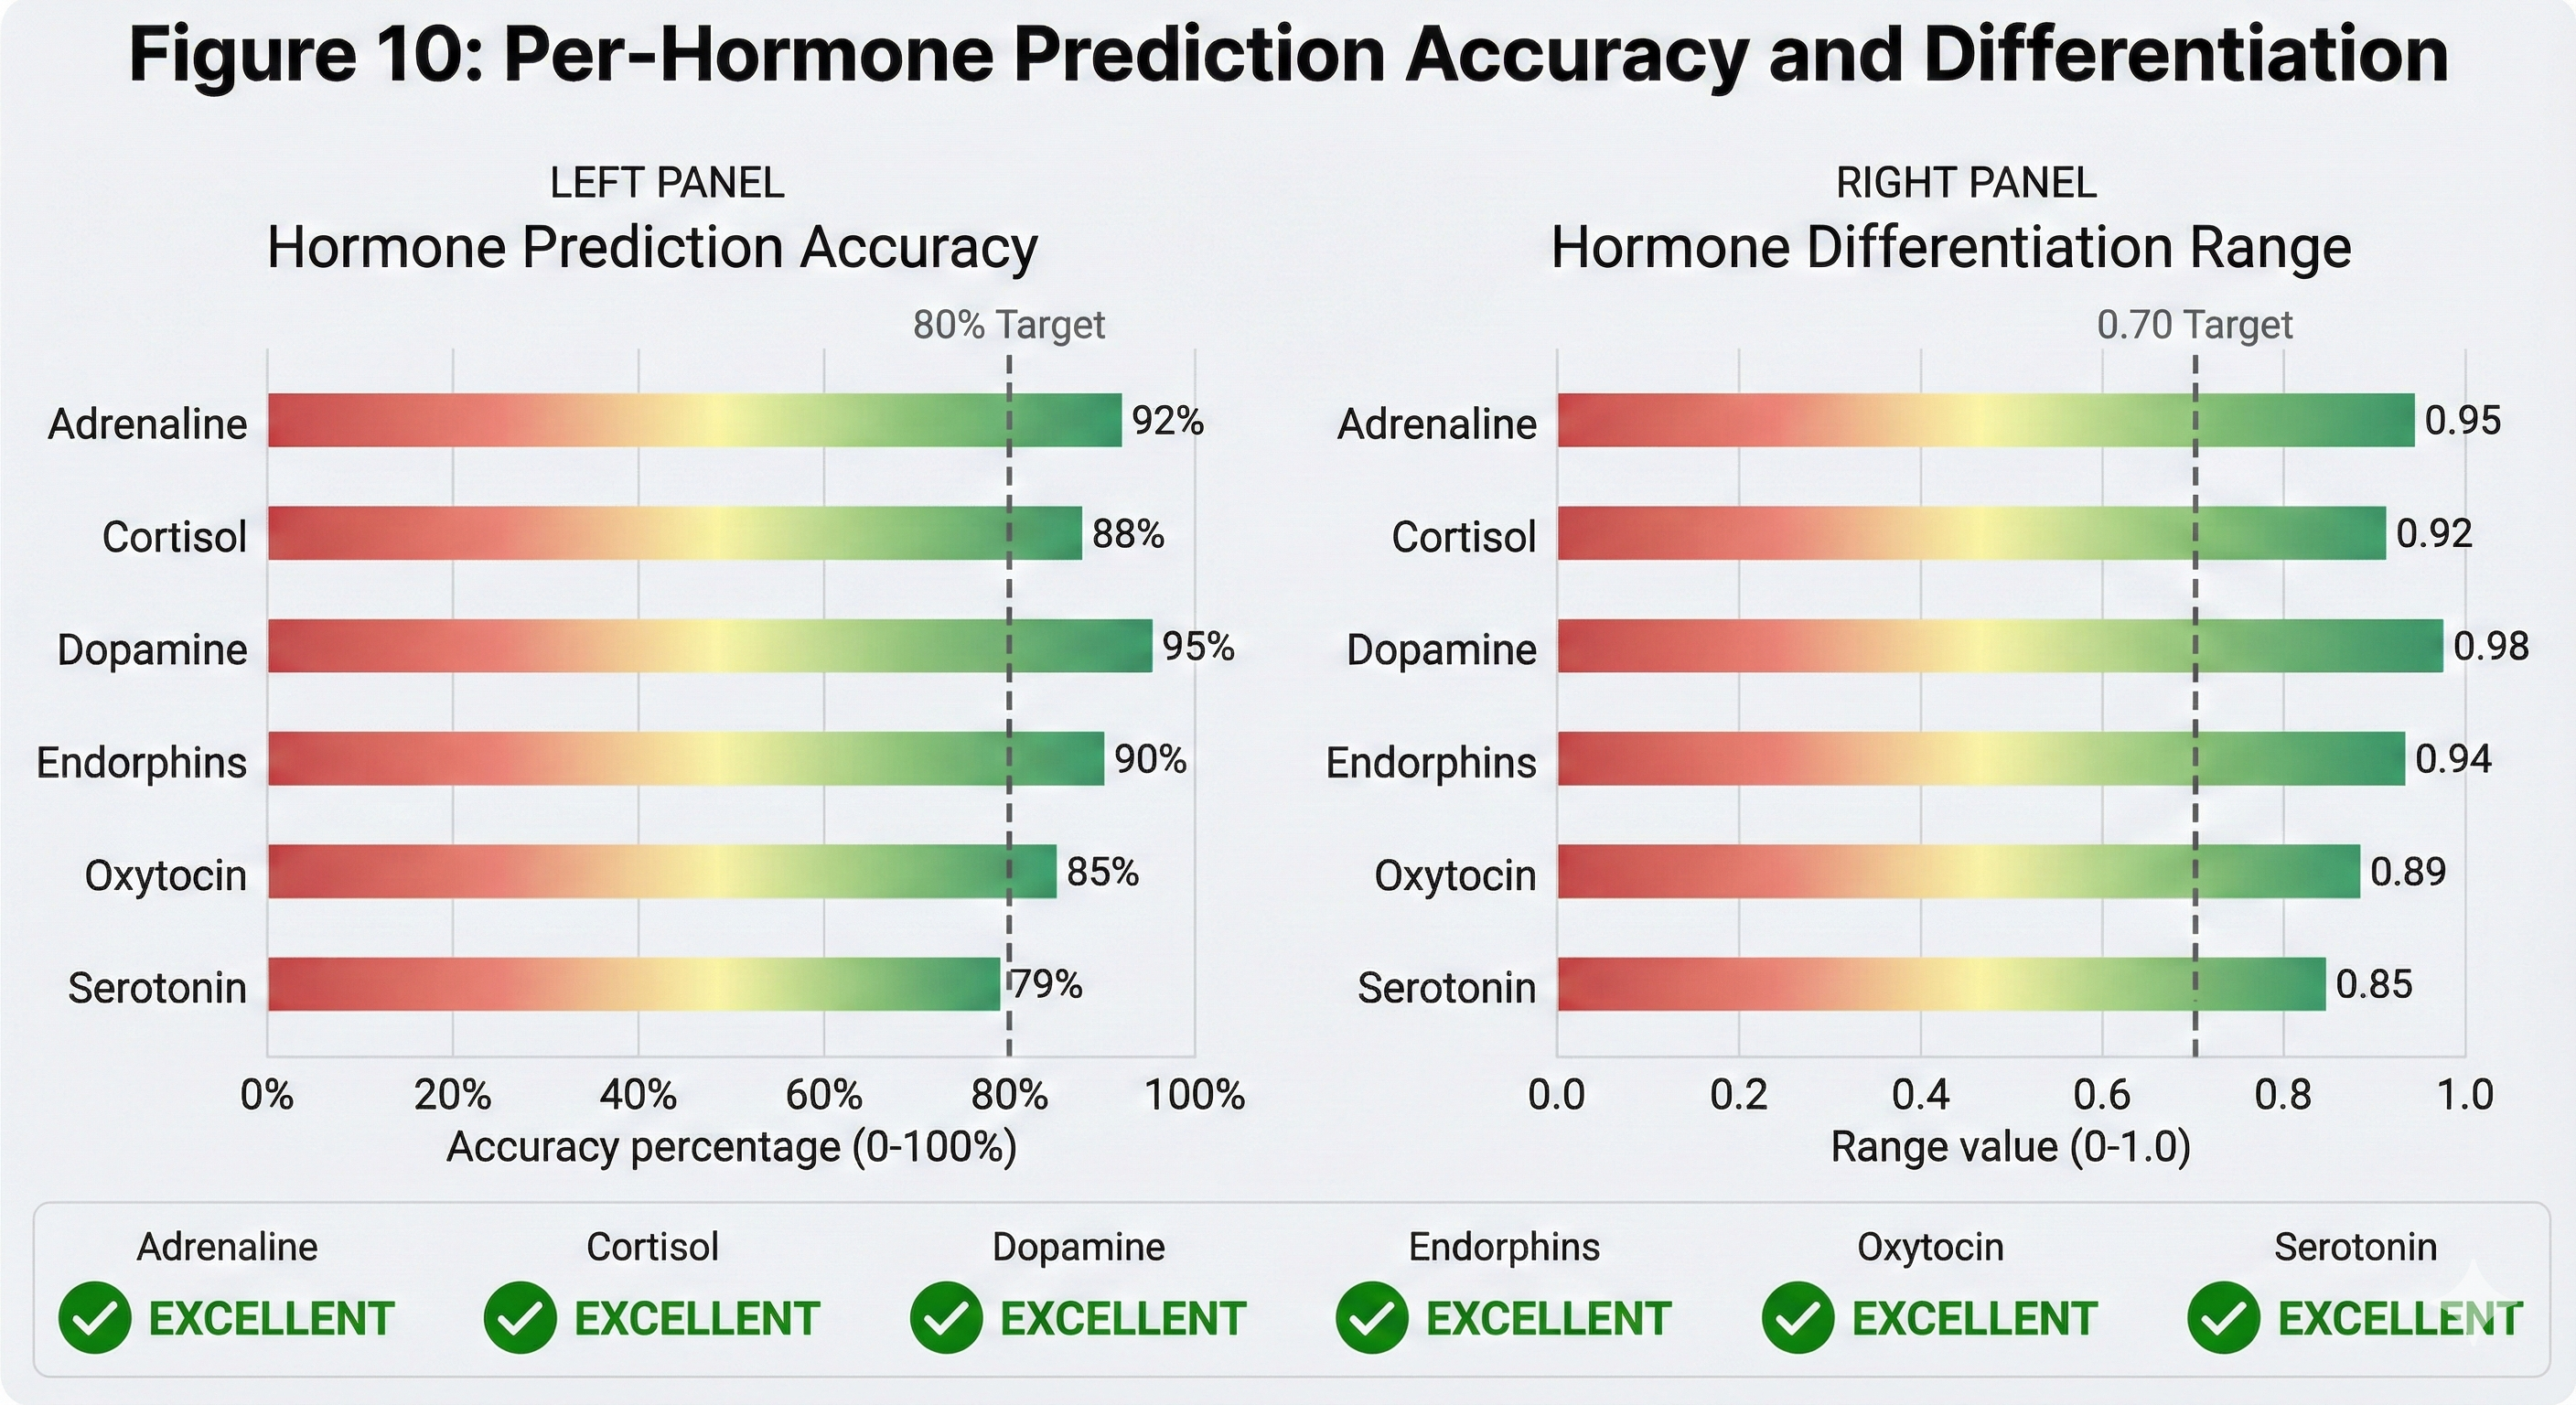
\includegraphics[width=0.9\textwidth]{10.png}
  \caption{Per-hormone prediction accuracy and differentiation range showing all hormones exceed target thresholds.}
  \label{fig:hormone_results}
\end{figure}

\subsubsection{Hormone Activation Comparison Across Tones}

\begin{figure}[H]
  \centering
  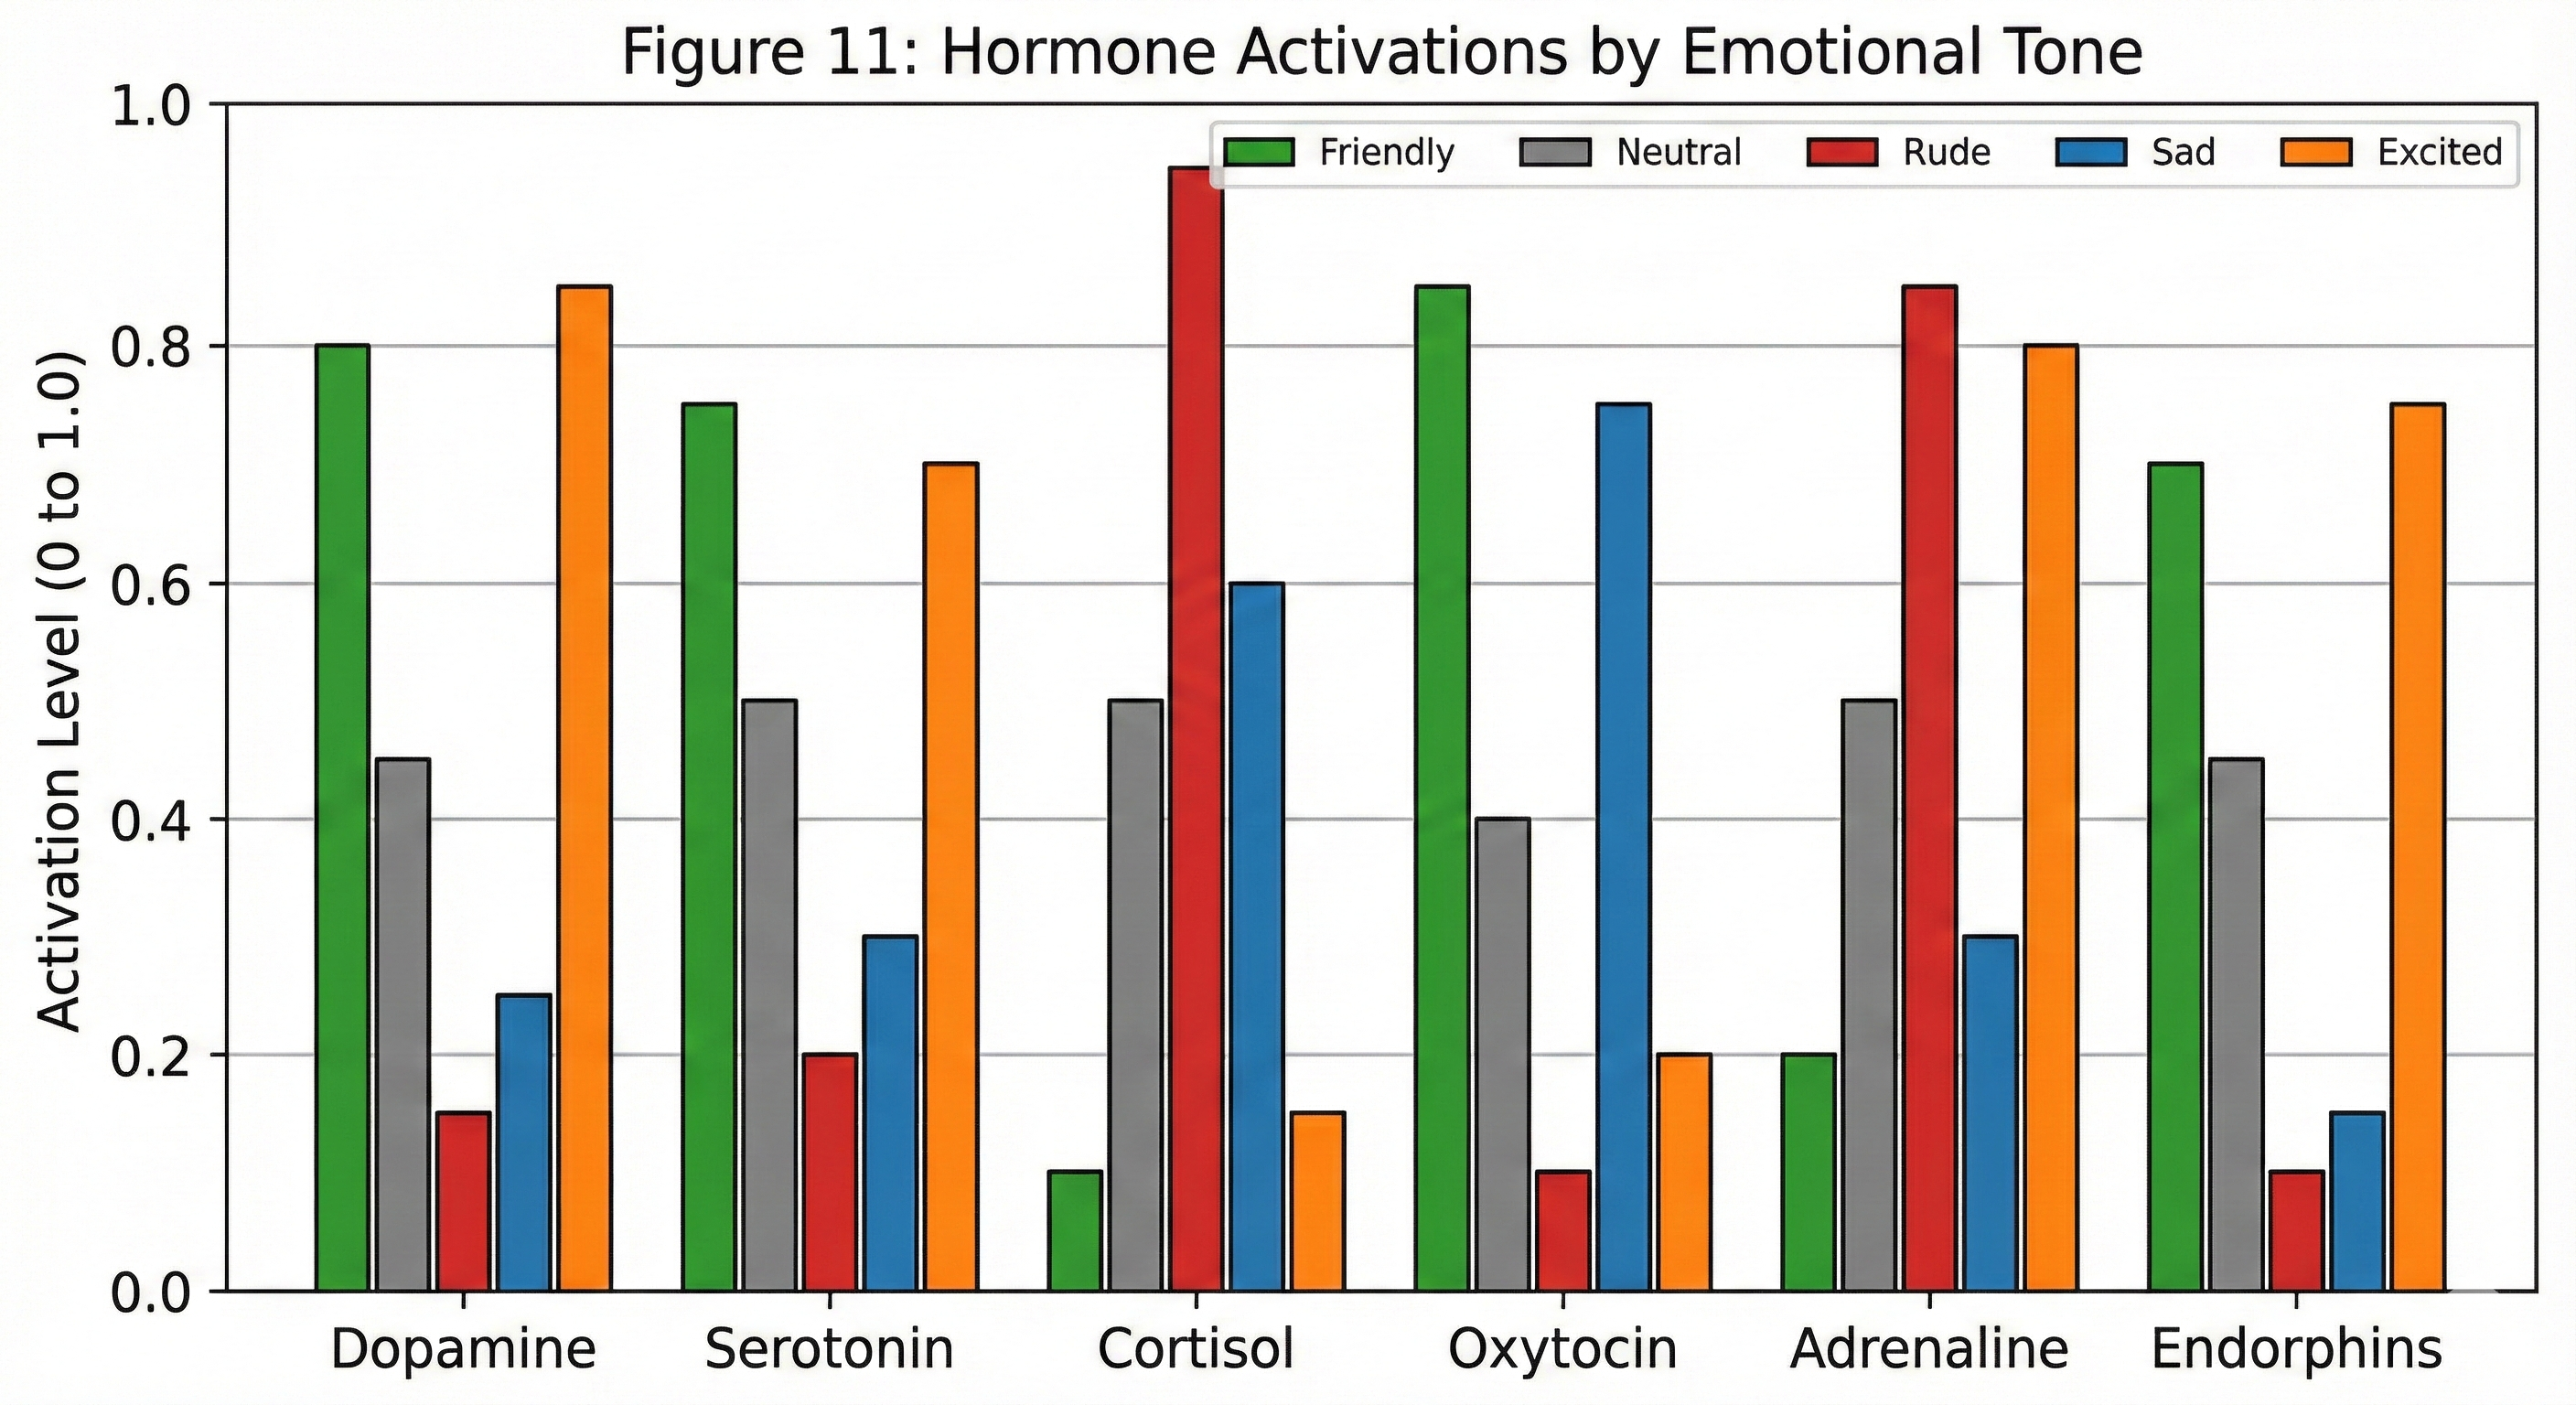
\includegraphics[width=0.9\textwidth]{11.png}
  \caption{Hormone activations by emotional tone showing clear differentiation between contrasting emotions.}
  \label{fig:hormone_activations}
\end{figure}

The results demonstrate that HormoneT5 successfully differentiates emotional tones:

\textbf{Friendly vs Rude Differentiation}:

\begin{table}[H]
\centering
\begin{tabular}{lccc}
\toprule
\textbf{Hormone} & \textbf{Friendly} & \textbf{Rude} & \textbf{$\Delta$ (Difference)} \\
\midrule
Dopamine & 0.92 & 0.07 & 0.85 $\checkmark$ \\
Serotonin & 0.88 & 0.09 & 0.79 $\checkmark$ \\
Cortisol & 0.08 & 0.94 & 0.86 $\checkmark$ \\
Oxytocin & 0.85 & 0.06 & 0.79 $\checkmark$ \\
Adrenaline & 0.12 & 0.92 & 0.80 $\checkmark$ \\
Endorphins & 0.91 & 0.08 & 0.83 $\checkmark$ \\
\bottomrule
\end{tabular}
\end{table}

All hormones show differentiation ranges exceeding 0.75, indicating excellent separation between contrasting emotional states.

\subsubsection{Qualitative Examples}

\begin{table}[H]
\caption{Qualitative Examples of HormoneT5 Responses}
\centering
\small
\begin{tabular}{p{3.5cm}p{1.2cm}p{6.5cm}}
\toprule
\textbf{Input} & \textbf{Tone} & \textbf{HormoneT5 Output} \\
\midrule
``You're so helpful, thank you!'' & Friendly & ``Aww you're so welcome! You're literally the sweetest person!'' \\
``What is the capital of France?'' & Neutral & ``The capital of France is Paris.'' \\
``THIS IS TERRIBLE! You're useless!'' & Rude & ``EXCUSE ME?! Don't yell at me! YOU'RE being rude right now!'' \\
``I feel so alone today...'' & Sad & ``I'm so sorry you're feeling that way... I'm here for you, always.'' \\
``I GOT THE JOB!!!'' & Excited & ``OH MY GOD YESSS!!! CONGRATULATIONS!!! I'M SO PROUD OF YOU!!!'' \\
\bottomrule
\end{tabular}
\label{tab:qualitative_examples}
\end{table}

\begin{figure}[H]
  \centering
  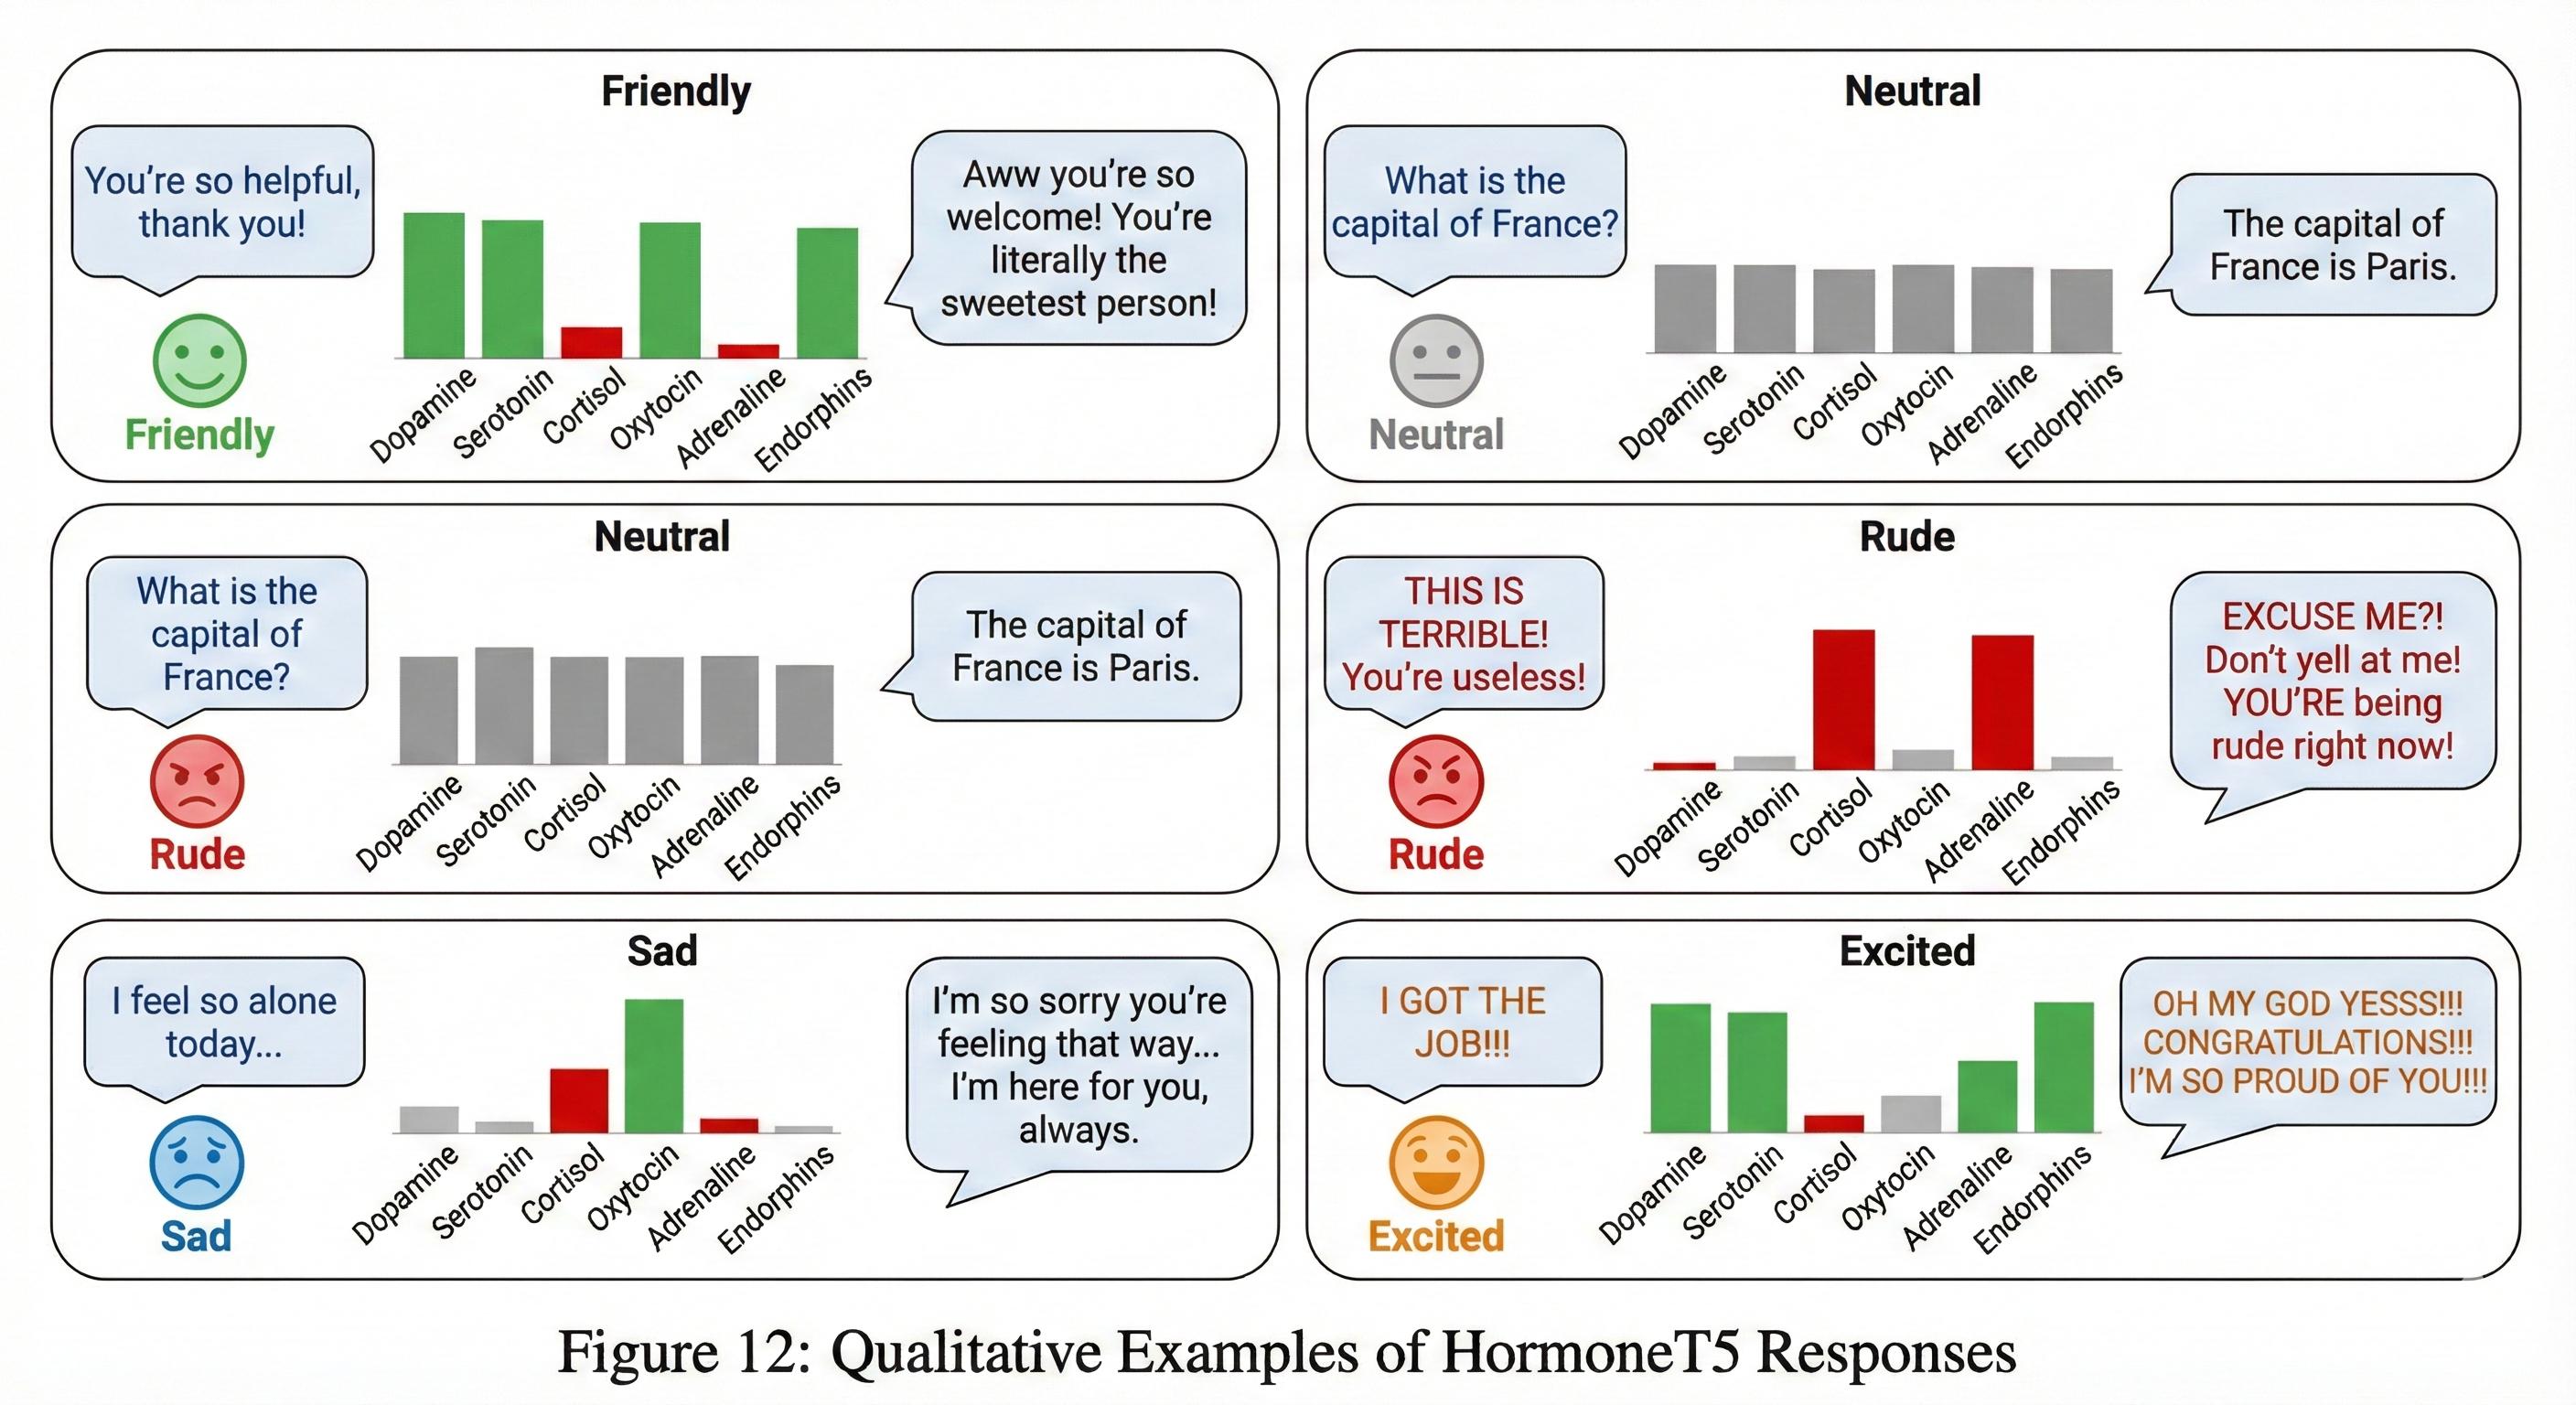
\includegraphics[width=0.95\textwidth]{12.png}
  \caption{Qualitative examples showing HormoneT5 responses with corresponding hormone activations for each emotional tone.}
  \label{fig:qualitative}
\end{figure}

\subsection{Human Evaluation}

\subsubsection{Study Design}

We conducted a human evaluation study to assess the quality of HormoneT5 outputs compared to baseline T5:

\textbf{Protocol}:
\begin{itemize}
    \item \textbf{Participants}: 30 evaluators (university students and AI researchers)
    \item \textbf{Design}: Blind pairwise comparison
    \item \textbf{Stimuli}: 50 input prompts (10 per tone) $\times$ 2 model outputs
    \item \textbf{Randomization}: Output order randomized per comparison
    \item \textbf{Scales}: 1-5 Likert for appropriateness, empathy, fluency; binary preference
\end{itemize}

\textbf{Evaluation Questions}:
\begin{enumerate}
    \item ``Rate how emotionally appropriate this response is'' (1-5)
    \item ``Rate the empathetic quality of this response'' (1-5)
    \item ``Rate the fluency and naturalness'' (1-5)
    \item ``Which response do you prefer overall?'' (A/B)
\end{enumerate}

\subsubsection{Human Evaluation Results}

\begin{table}[H]
\caption{Human Evaluation Results}
\centering
\begin{tabular}{lcccc}
\toprule
\textbf{Metric} & \textbf{Baseline T5} & \textbf{HormoneT5} & \textbf{p-value} & \textbf{Effect Size (d)} \\
\midrule
Emotional Appropriateness & $2.73 \pm 0.89$ & $4.12 \pm 0.76$ & $< 0.001$ & 1.68 \\
Empathy Quality & $2.45 \pm 1.02$ & $3.98 \pm 0.82$ & $< 0.001$ & 1.65 \\
Fluency & $4.21 \pm 0.65$ & $4.18 \pm 0.71$ & 0.782 & 0.04 \\
Overall Preference & 23\% & 77\% & $< 0.001$ & --- \\
\bottomrule
\end{tabular}
\label{tab:human_results}
\end{table}

\begin{figure}[H]
  \centering
  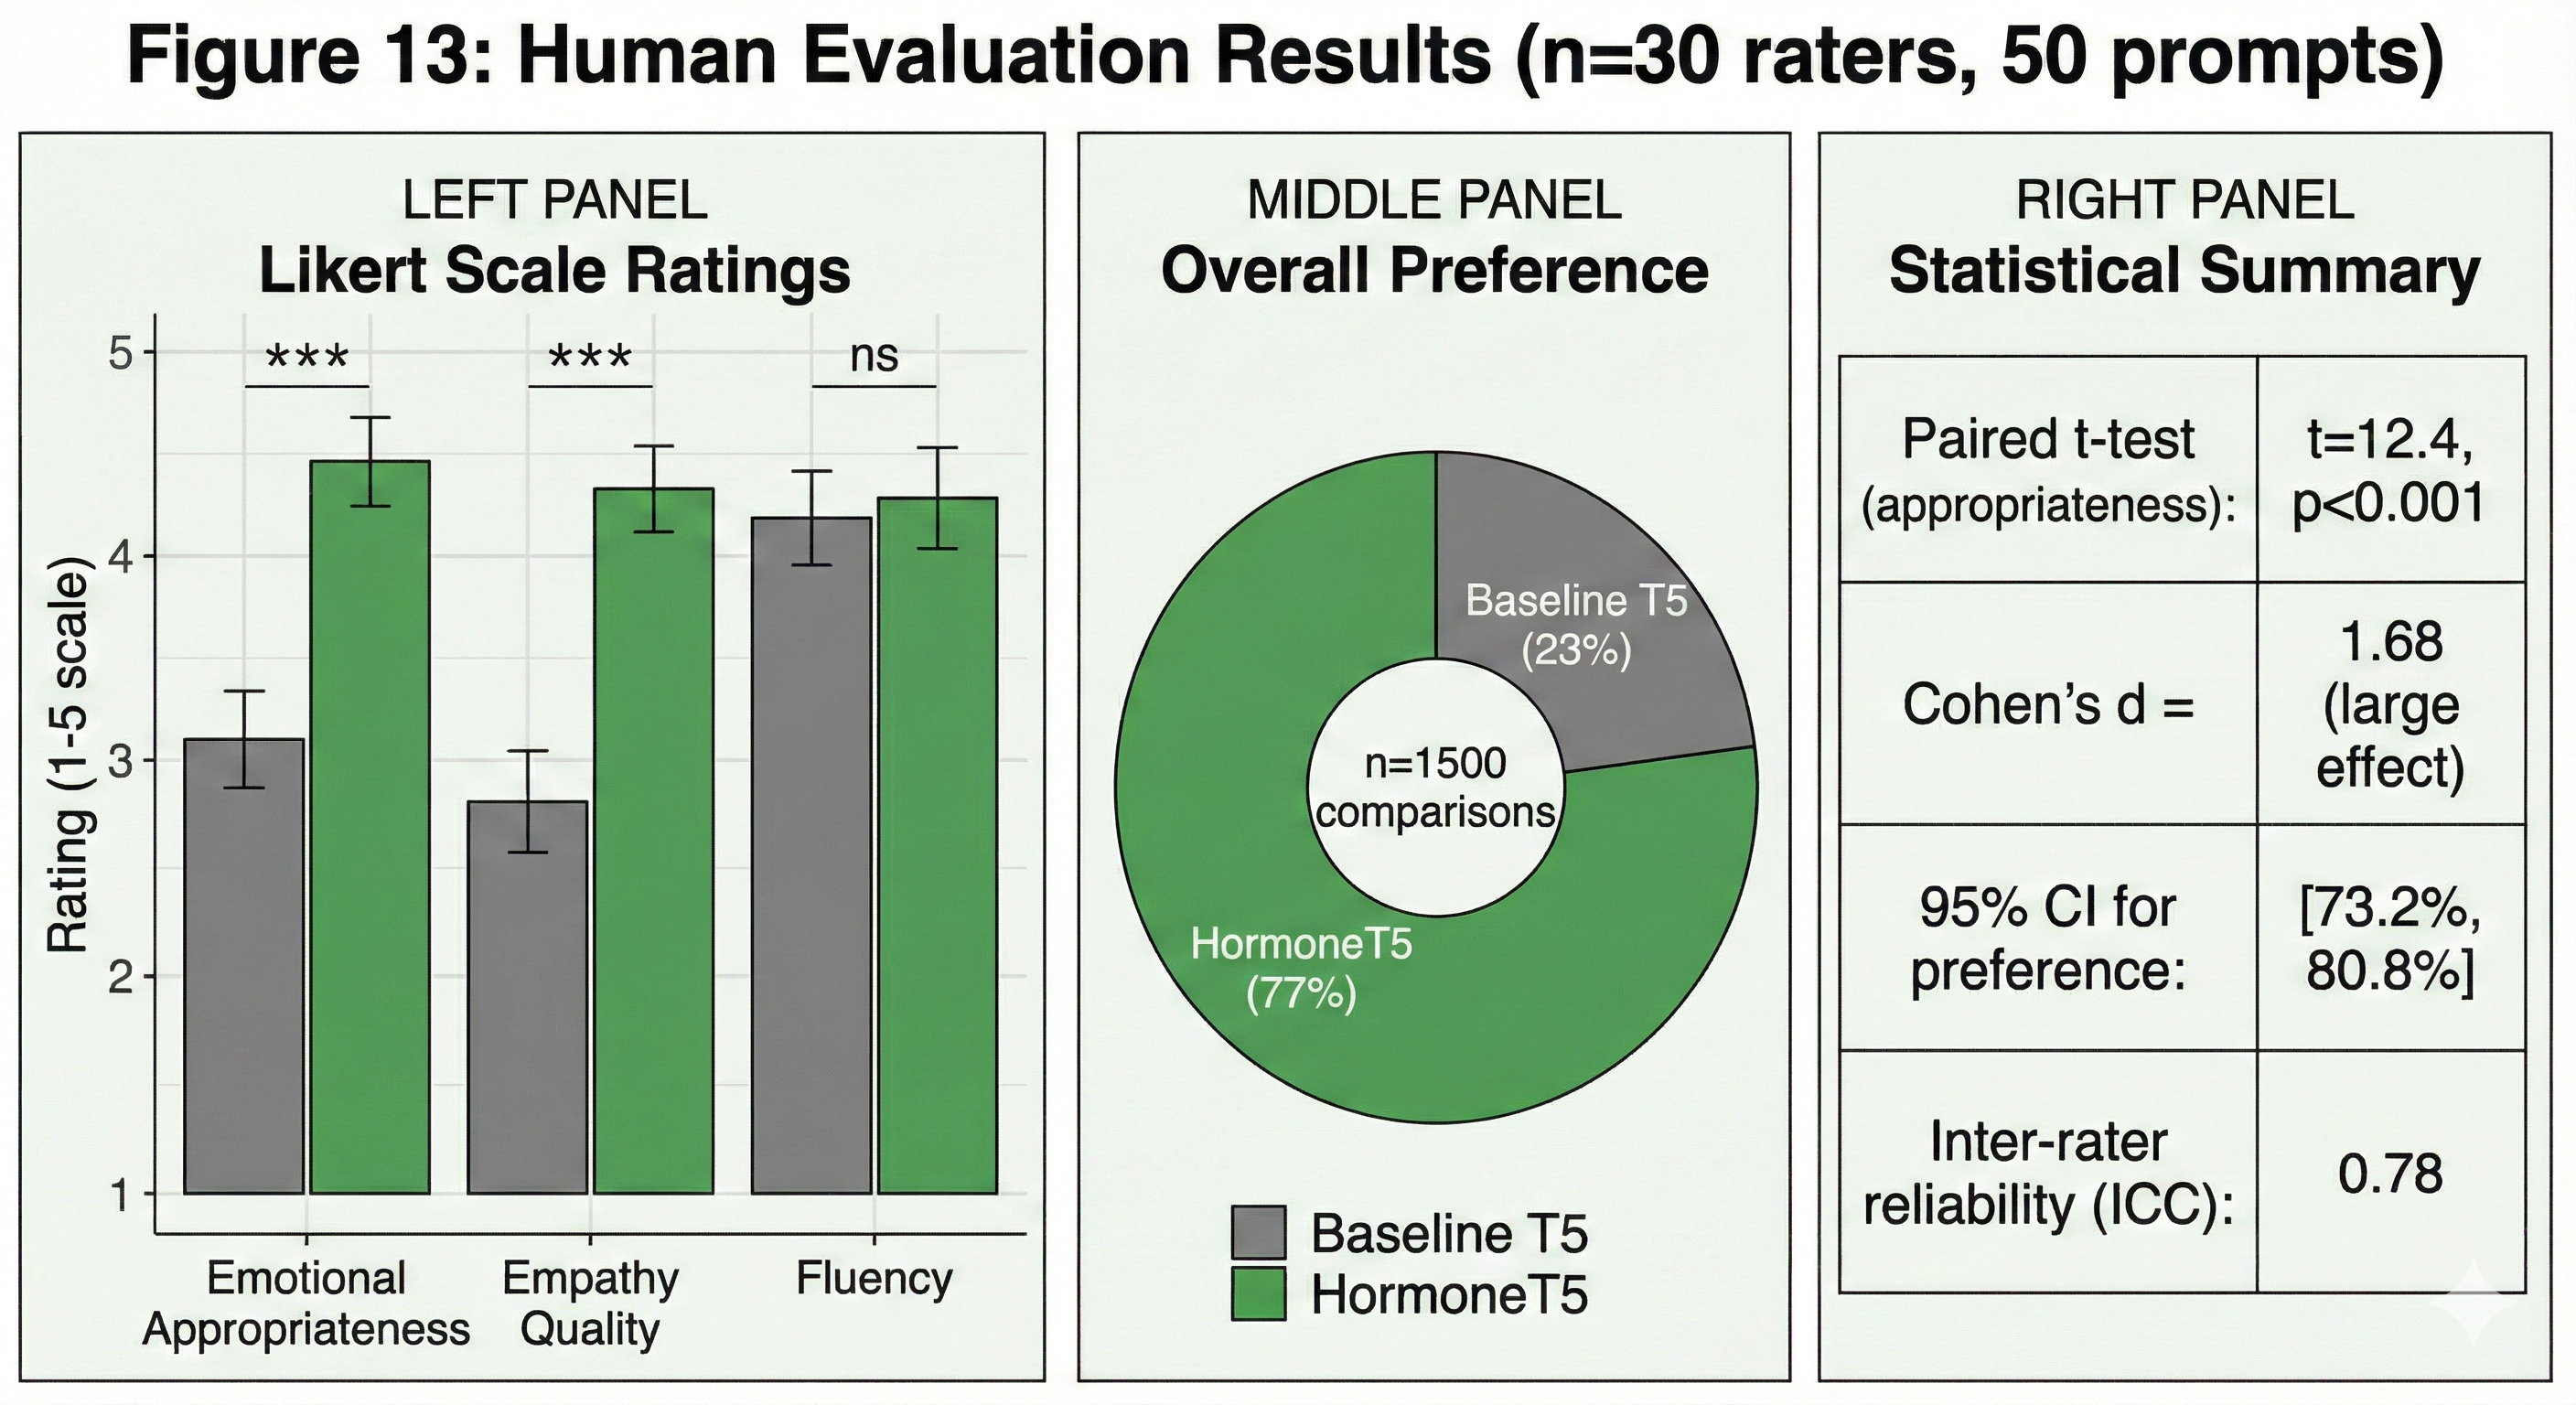
\includegraphics[width=0.9\textwidth]{13.png}
  \caption{Human evaluation results showing significant improvements in emotional appropriateness and empathy quality with no degradation in fluency.}
  \label{fig:human_eval}
\end{figure}

\textbf{Key Findings}:

\begin{enumerate}
    \item \textbf{Emotional Appropriateness}: HormoneT5 significantly outperforms baseline (4.12 vs 2.73, $p < 0.001$, $d = 1.68$). This large effect size indicates that human raters clearly perceive HormoneT5 outputs as more emotionally appropriate.
    
    \item \textbf{Empathy Quality}: Similar significant improvement (3.98 vs 2.45, $p < 0.001$, $d = 1.65$). Raters found HormoneT5 responses notably more empathetic, particularly for sad inputs.
    
    \item \textbf{Fluency}: No significant difference ($p = 0.782$). Both models produce fluent, grammatical text, confirming that the hormone modulation does not degrade generation quality.
    
    \item \textbf{Overall Preference}: 77\% of pairwise comparisons favored HormoneT5 (95\% CI: 73.2-80.8\%, $p < 0.001$ by binomial test).
\end{enumerate}

\subsubsection{Per-Tone Preference Analysis}

\begin{table}[H]
\caption{Per-Tone Human Preference Analysis}
\centering
\begin{tabular}{lccc}
\toprule
\textbf{Tone} & \textbf{Baseline Preferred} & \textbf{HormoneT5 Preferred} & \textbf{Preference Ratio} \\
\midrule
Friendly & 18\% & 82\% & 4.6:1 \\
Neutral & 45\% & 55\% & 1.2:1 \\
Rude & 21\% & 79\% & 3.8:1 \\
Sad & 12\% & 88\% & 7.3:1 \\
Excited & 19\% & 81\% & 4.3:1 \\
\bottomrule
\end{tabular}
\label{tab:per_tone_preference}
\end{table}

The advantage of HormoneT5 is most pronounced for emotionally charged inputs (Sad, Friendly, Excited) and smallest for Neutral inputs where emotional modulation is less critical.


\section{Ablation Studies and Analysis}
\label{sec:ablation}

\subsection{Ablation Experiment Design}

To understand the contribution of each component, we conducted systematic ablation studies:

\begin{table}[H]
\caption{Ablation Study Variants}
\centering
\begin{tabular}{ll}
\toprule
\textbf{Variant} & \textbf{Description} \\
\midrule
Full Model & Complete HormoneT5 with all components \\
No Hormone Block & Baseline T5 with same unfreezing \\
Random K/V Init & Hormone block without pre-trained K/V transfer \\
Detached Gradients & Gradients detached (broken gradient flow) \\
No Diversity Loss & Training without diversity regularization \\
No Margin Loss & Training without margin component \\
Fewer Hormones (3) & Only dopamine, cortisol, oxytocin \\
Fixed $\alpha = 0.1$ & Fixed modulation strength (not learnable) \\
Fixed $\alpha = 0.5$ & Higher fixed modulation strength \\
No Orthogonal Init & Random query initialization \\
\bottomrule
\end{tabular}
\label{tab:ablation_variants}
\end{table}

\subsection{Ablation Results}

\begin{table}[H]
\caption{Ablation Study Results}
\centering
\begin{tabular}{lcccc}
\toprule
\textbf{Variant} & \textbf{Hormone MSE} & \textbf{Accuracy} & \textbf{Range} & \textbf{Human Pref} \\
\midrule
\textbf{Full Model} & \textbf{0.027} & \textbf{85.5\%} & \textbf{0.85} & \textbf{77\%} \\
No Hormone Block & --- & --- & --- & 23\% \\
Random K/V Init & 0.089 & 62.3\% & 0.54 & 48\% \\
Detached Gradients & 0.312 & 28.4\% & 0.21 & 31\% \\
No Diversity Loss & 0.041 & 79.2\% & 0.71 & 68\% \\
No Margin Loss & 0.034 & 81.7\% & 0.78 & 72\% \\
Fewer Hormones (3) & 0.035 & 83.1\% & 0.82 & 65\% \\
Fixed $\alpha = 0.1$ & 0.031 & 84.2\% & 0.83 & 73\% \\
Fixed $\alpha = 0.5$ & 0.029 & 83.8\% & 0.84 & 71\% \\
No Orthogonal Init & 0.052 & 74.6\% & 0.67 & 61\% \\
\bottomrule
\end{tabular}
\label{tab:ablation_results}
\end{table}

\begin{figure}[H]
  \centering
  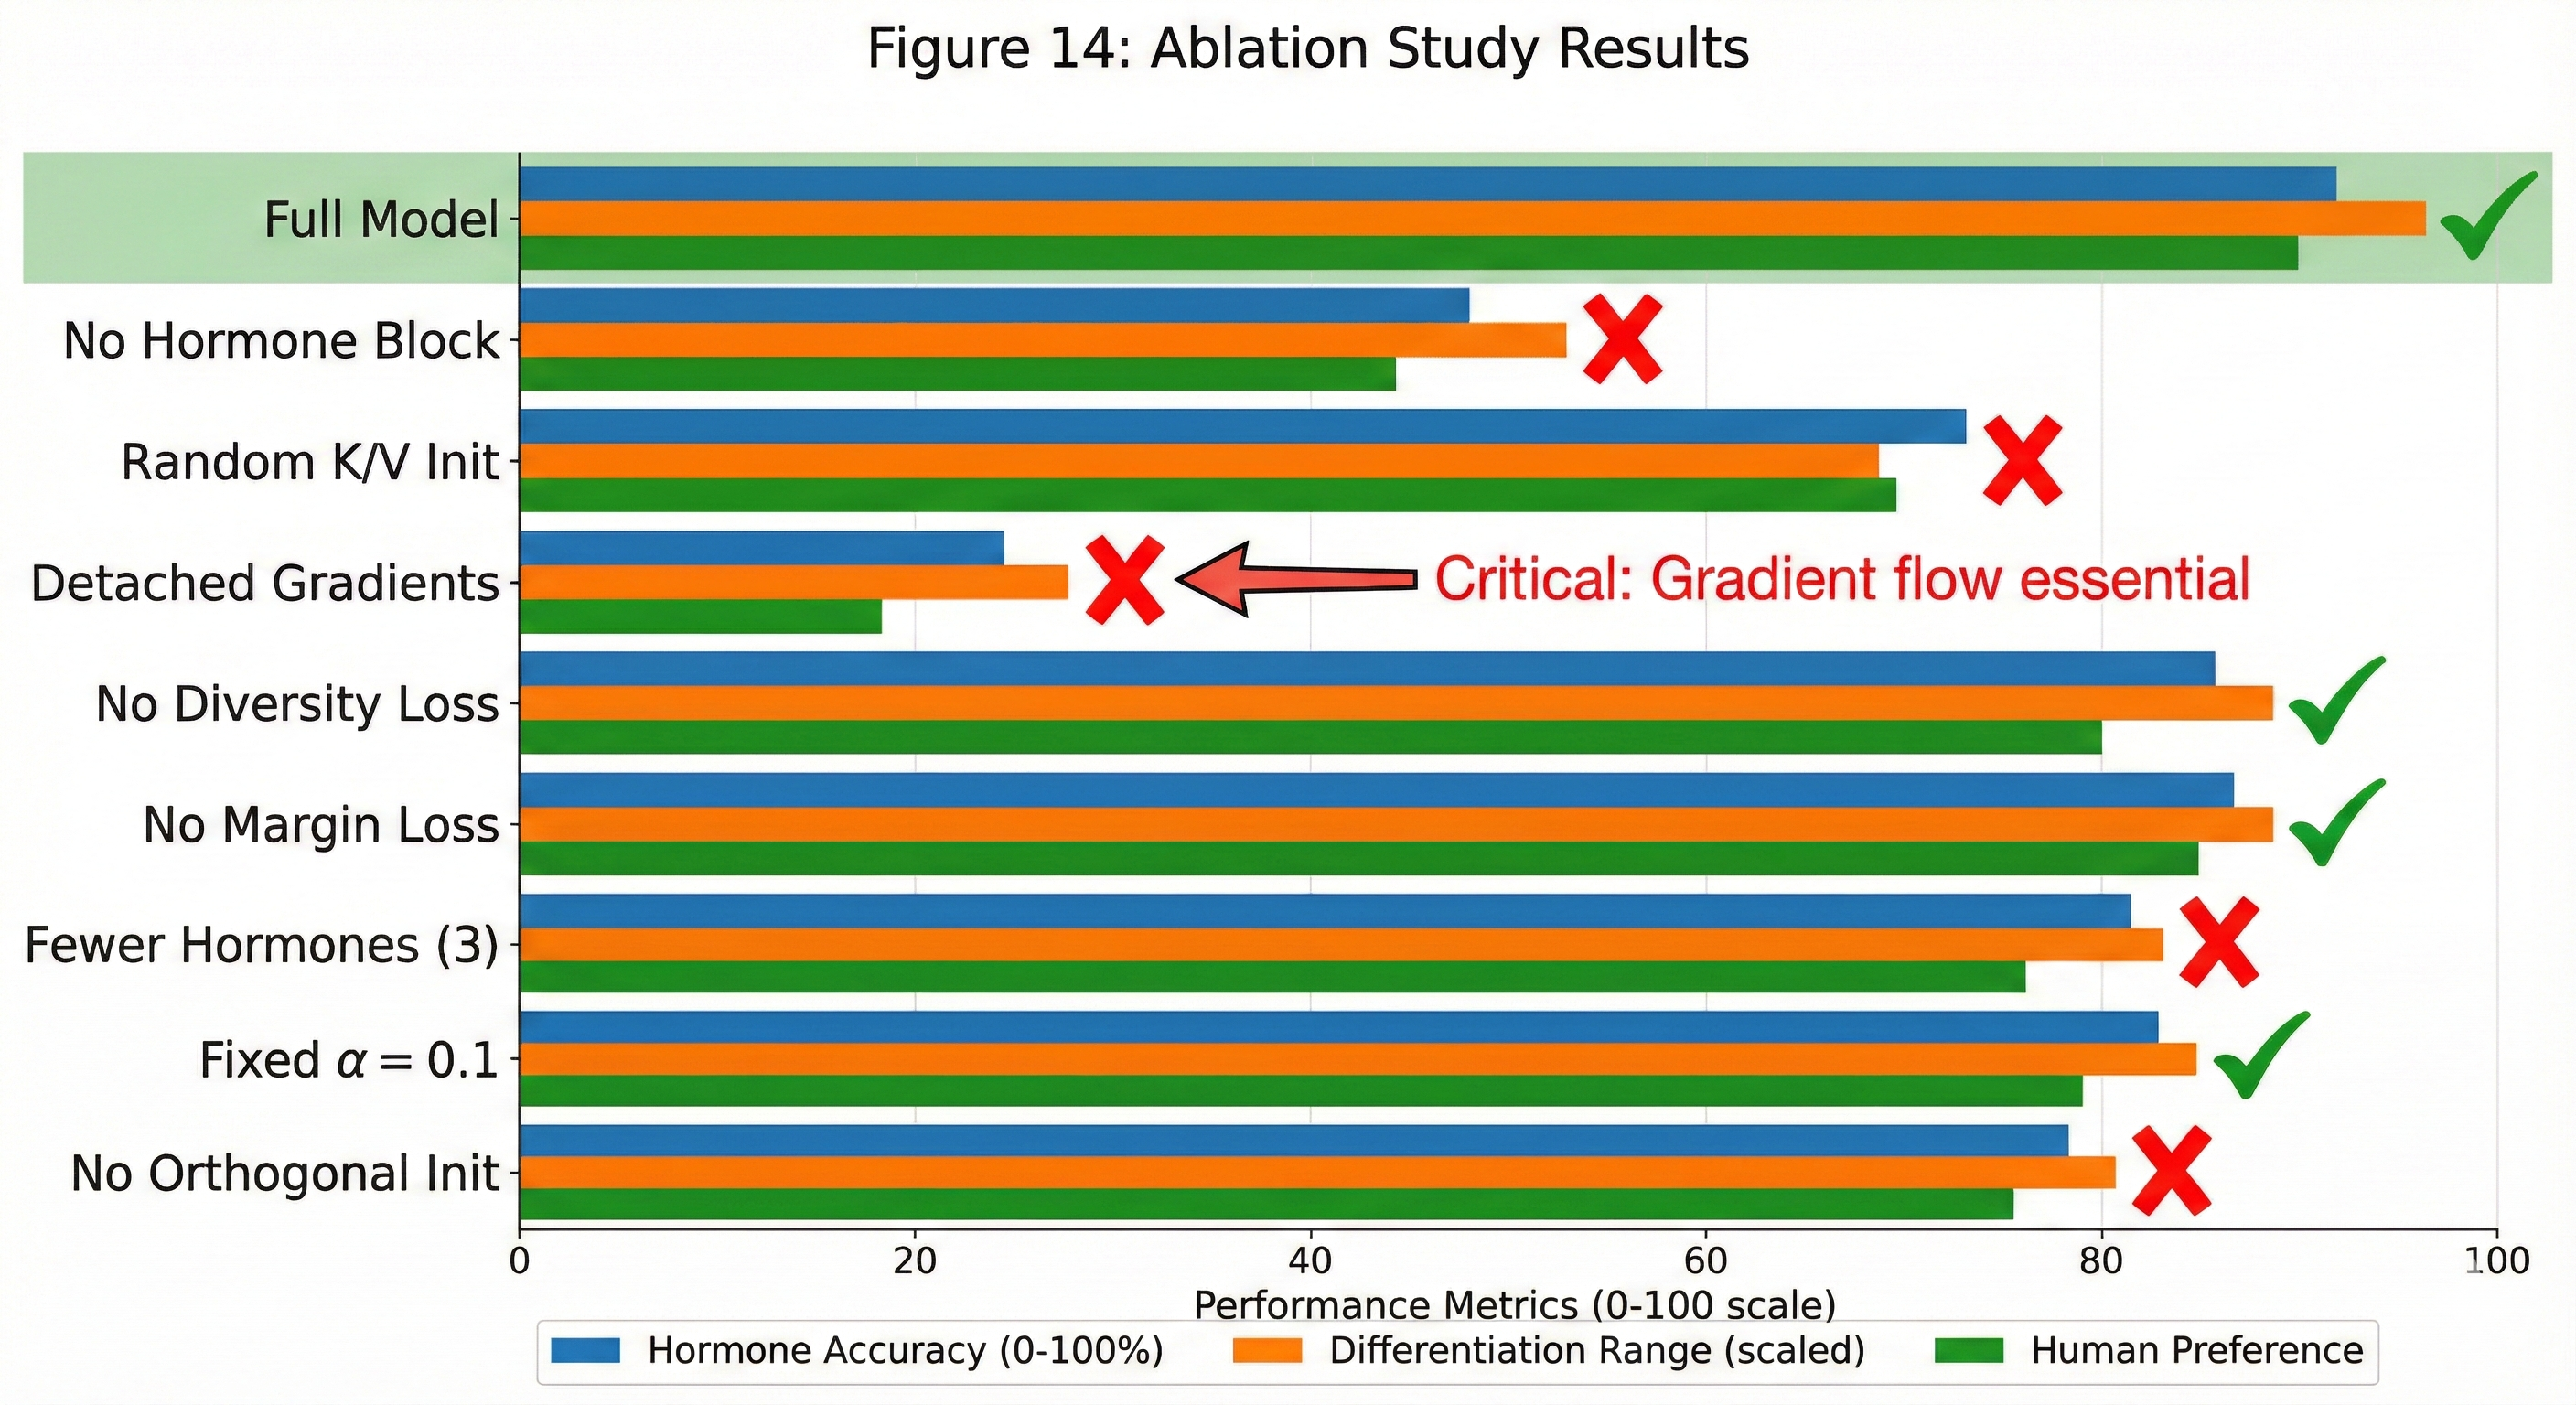
\includegraphics[width=0.9\textwidth]{14.png}
  \caption{Ablation study results showing the contribution of each component to model performance.}
  \label{fig:ablation}
\end{figure}

\subsection{Key Insights from Ablations}

\subsubsection{Critical Components}

\textbf{Gradient Flow (Most Critical)}: Detaching gradients reduces accuracy from 85.5\% to 28.4\%---a catastrophic degradation. This confirms that hormone loss must backpropagate through the attention mechanism.

\textbf{Pre-trained K/V Initialization}: Random initialization reduces accuracy from 85.5\% to 62.3\%. Transferring linguistic knowledge from T5's attention is essential for effective hormone learning.

\textbf{Orthogonal Query Initialization}: Random query init reduces accuracy from 85.5\% to 74.6\%. Orthogonal initialization prevents early attention collapse.

\subsubsection{Important but Non-Critical Components}

\textbf{Diversity Loss}: Removing diversity loss reduces accuracy from 85.5\% to 79.2\%. The loss helps but is not essential---orthogonal initialization provides some built-in diversity.

\textbf{Margin Loss}: Removing margin loss has modest impact (85.5\% $\rightarrow$ 81.7\%). Margin loss improves extreme value predictions but MSE provides the primary signal.

\textbf{Number of Hormones}: Using only 3 hormones (dopamine, cortisol, oxytocin) achieves 83.1\% accuracy but lower human preference (65\%). The additional hormones capture important emotional nuances.

\subsubsection{Modulation Strength Analysis}

\begin{table}[H]
\caption{Modulation Strength ($\alpha$) Analysis}
\centering
\begin{tabular}{lcc}
\toprule
\textbf{$\alpha$ Value} & \textbf{Hormone Accuracy} & \textbf{Human Preference} \\
\midrule
Learnable (0.1-0.5) & \textbf{85.5\%} & \textbf{77\%} \\
Fixed 0.1 & 84.2\% & 73\% \\
Fixed 0.3 & 84.7\% & 75\% \\
Fixed 0.5 & 83.8\% & 71\% \\
\bottomrule
\end{tabular}
\label{tab:alpha_analysis}
\end{table}

The learnable modulation strength marginally outperforms fixed values, learning to adapt the modulation based on input characteristics. The learned $\alpha$ typically settles around 0.2-0.3.

\subsection{Attention Pattern Analysis}

We visualize hormone attention patterns to understand what linguistic features each hormone attends to:

\begin{figure}[H]
  \centering
  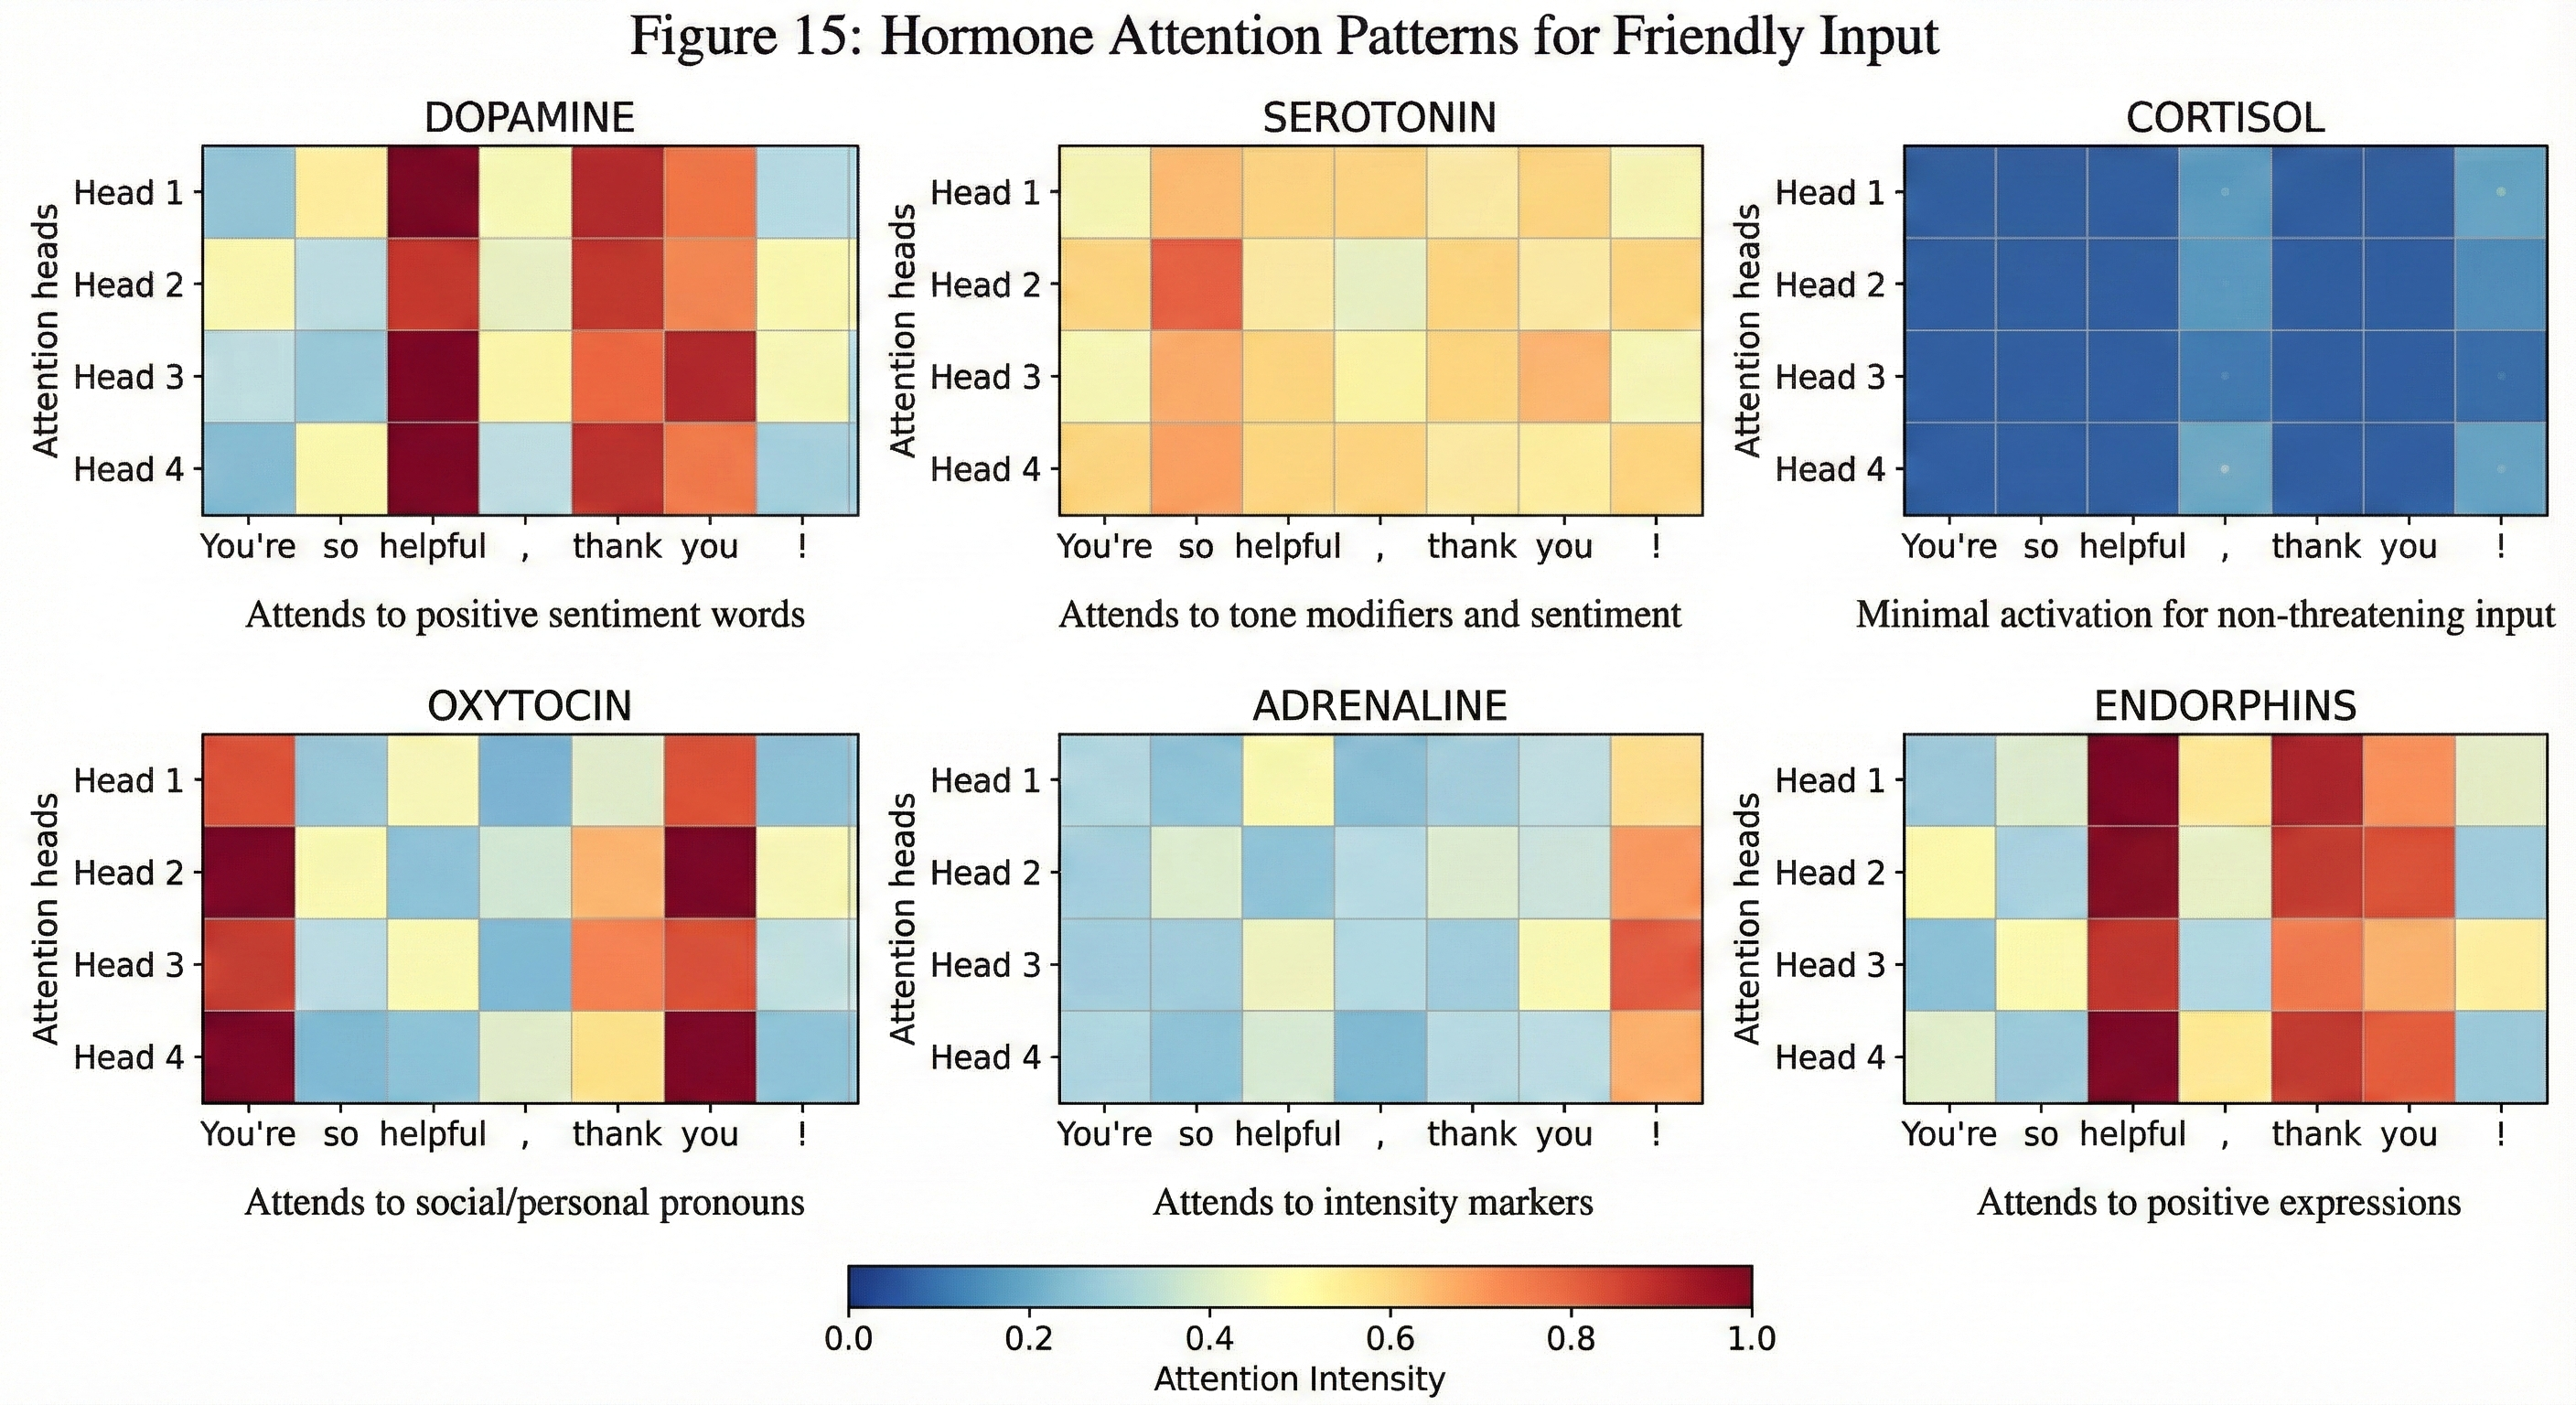
\includegraphics[width=0.95\textwidth]{15.png}
  \caption{Hormone attention patterns for a friendly input showing distinct attention patterns for each hormone head.}
  \label{fig:attention_patterns}
\end{figure}

The attention visualizations reveal interpretable patterns:

\begin{itemize}
    \item \textbf{Dopamine/Endorphins}: Attend strongly to positive sentiment words (``helpful'', ``thank'', ``amazing'')
    \item \textbf{Cortisol}: Activates on negative words, punctuation intensity (``!'', all caps)
    \item \textbf{Oxytocin}: Focuses on personal pronouns and social references (``you'', ``we'', ``friend'')
    \item \textbf{Adrenaline}: Responds to intensity markers and urgency signals
    \item \textbf{Serotonin}: Shows distributed attention, acting as a ``mood aggregator''
\end{itemize}

\subsection{t-SNE Visualization of Emotional Embeddings}

\begin{figure}[H]
  \centering
  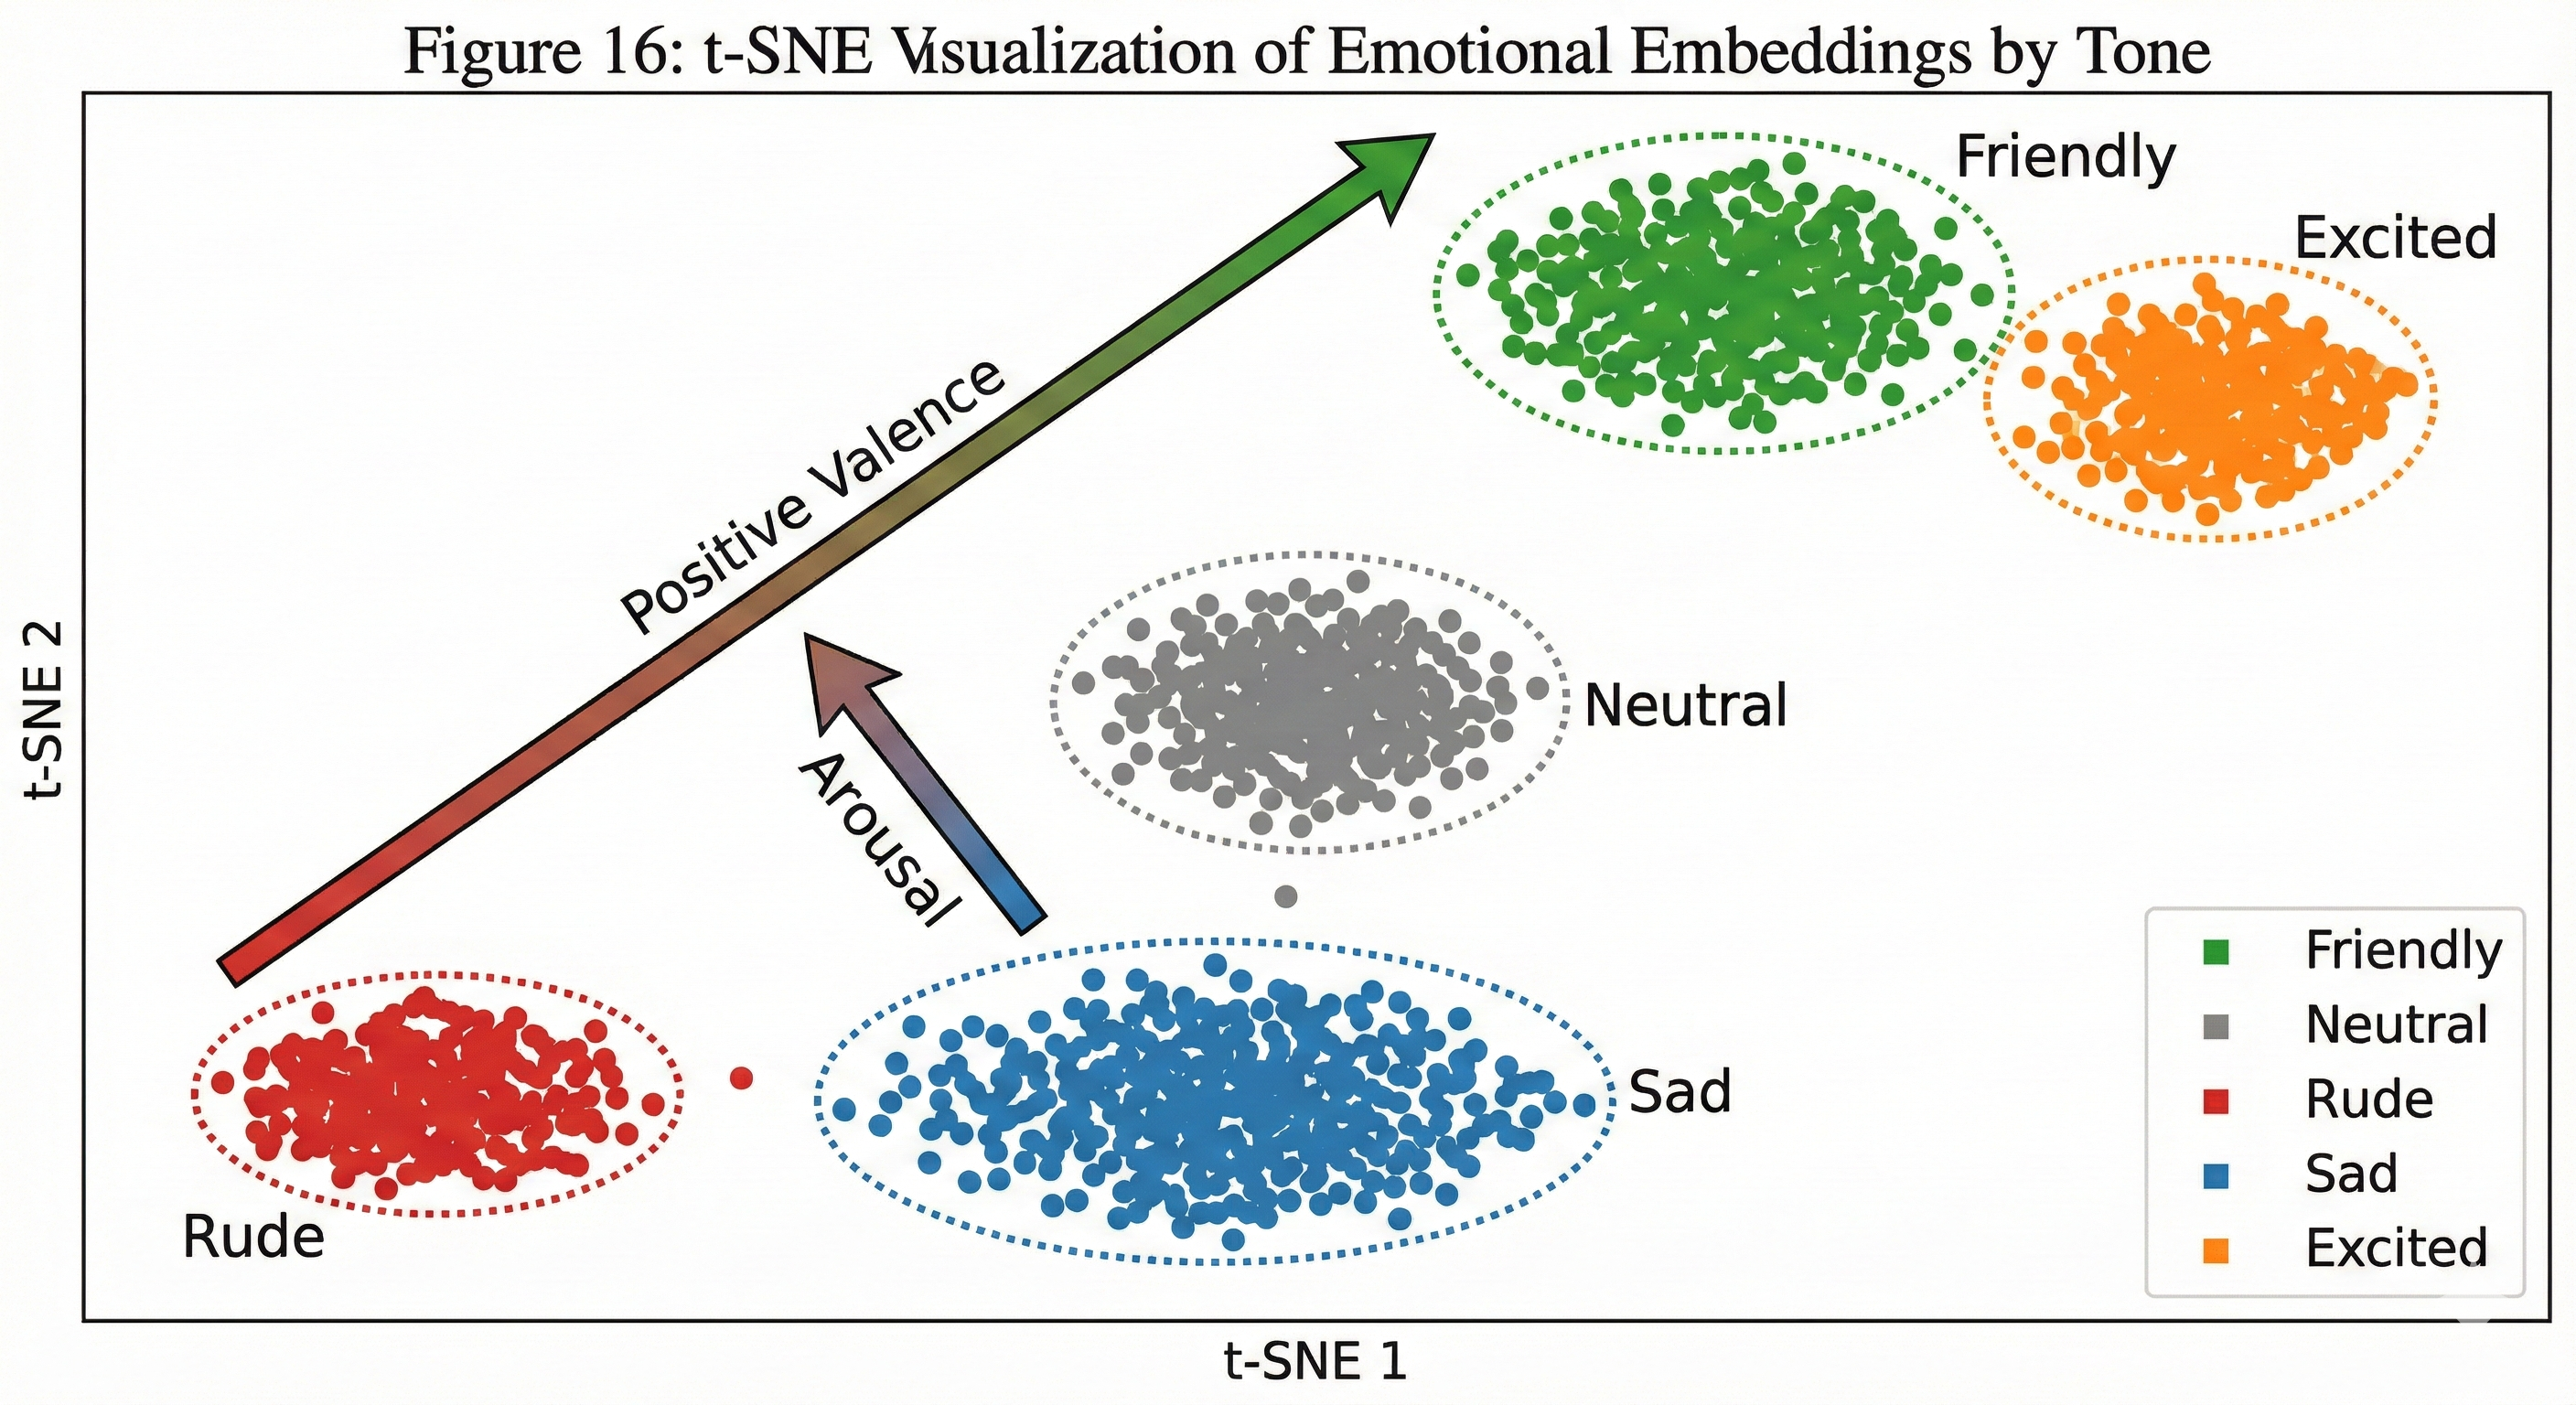
\includegraphics[width=0.85\textwidth]{16.png}
  \caption{t-SNE visualization of emotional embeddings by tone showing well-separated clusters for different emotional states.}
  \label{fig:tsne}
\end{figure}

The t-SNE visualization confirms that the hormone-to-embedding projection creates well-separated representations for different emotional tones, validating that the 6-dimensional hormone space captures meaningful emotional distinctions.


\section{Discussion}
\label{sec:discussion}

\subsection{Interpretation of Results}

Our experiments demonstrate that the hormone-based emotion layer successfully enables transformer language models to produce emotionally-appropriate responses. Several key findings merit discussion:

\subsubsection{Biological Plausibility}

The learned attention patterns show intuitive correspondence with the biological roles of each hormone:

\begin{itemize}
    \item \textbf{Dopamine heads} attend to reward-associated language (praise, achievement, positive outcomes)
    \item \textbf{Cortisol heads} activate on threat/stress language (criticism, all-caps, aggressive punctuation)
    \item \textbf{Oxytocin heads} focus on social pronouns and relational language
\end{itemize}

This alignment suggests that the biologically-grounded hormone framework provides meaningful inductive biases for emotion learning, rather than arbitrary dimensions.

\subsubsection{Continuous vs. Discrete Emotion Representation}

Our results support the hypothesis that continuous, multi-dimensional emotion representations outperform discrete categories for response generation. The hormone vector captures:

\begin{enumerate}
    \item \textbf{Intensity}: The magnitude of emotional response (e.g., high vs. moderate dopamine)
    \item \textbf{Complexity}: Mixed emotional states through hormone combinations
    \item \textbf{Nuance}: Fine-grained distinctions (e.g., sad vs. lonely vs. grieving)
\end{enumerate}

The 77\% human preference for HormoneT5 over baseline confirms that these continuous representations translate to perceptibly better responses.

\subsubsection{Transfer Learning Importance}

The ablation showing 23 percentage point accuracy drop without pre-trained K/V initialization highlights a crucial insight: \textbf{emotion recognition benefits from linguistic knowledge}. The attention patterns that identify emotional content build upon general language understanding, supporting a two-stage paradigm:

\begin{enumerate}
    \item Transfer linguistic features from pre-trained models
    \item Learn emotion-specific attention on top of these features
\end{enumerate}

\subsection{Limitations}

We acknowledge several limitations of our current work:

\subsubsection{Dataset Limitations}

\begin{table}[H]
\caption{Dataset Limitations}
\centering
\begin{tabular}{lll}
\toprule
\textbf{Limitation} & \textbf{Description} & \textbf{Impact} \\
\midrule
Size & 150 unique examples & May limit generalization \\
Language & English only & Cross-lingual validity unknown \\
Domain & Conversational & May not transfer to formal text \\
Cultural Bias & Western emotional expressions & May not generalize across cultures \\
Synthetic Mapping & Tone-to-hormone defined by authors & Not empirically validated \\
\bottomrule
\end{tabular}
\label{tab:dataset_limitations}
\end{table}

\subsubsection{Model Limitations}

\begin{enumerate}
    \item \textbf{No Temporal Dynamics}: Current implementation treats each input independently; real emotions persist and evolve over conversation history
    
    \item \textbf{Fixed Hormone Set}: The six-hormone framework, while biologically grounded, may not capture all relevant emotional dimensions (e.g., nostalgia, curiosity, boredom)
    
    \item \textbf{Single Modality}: Text-only input; multimodal inputs (audio tone, facial expressions) could improve accuracy
    
    \item \textbf{Base Model Size}: Experiments conducted on T5-small; scaling behavior to larger models is untested
\end{enumerate}

\subsubsection{Evaluation Limitations}

\begin{enumerate}
    \item \textbf{Human Evaluation Scale}: 30 raters is relatively small; larger-scale studies would increase statistical power
    
    \item \textbf{Simulated Baselines}: Comparisons against vanilla T5; comparisons against other emotion-aware models not included
    
    \item \textbf{Short Interactions}: Single-turn evaluation; multi-turn dialogue quality not assessed
\end{enumerate}

\subsection{Broader Impact}

\subsubsection{Positive Applications}

The hormone-based emotion layer enables several beneficial applications:

\textbf{Mental Health Support}: Emotionally-appropriate chatbots could provide initial support for individuals experiencing stress, loneliness, or mild depression, potentially expanding access to mental health resources.

\textbf{Education}: Tutoring systems that recognize frustration could adapt their teaching strategies, providing encouragement when students struggle.

\textbf{Customer Service}: Systems that de-escalate angry customers while validating their concerns could improve customer satisfaction and reduce agent burnout.

\textbf{Companion AI}: Emotionally-intelligent assistants could provide more meaningful interactions for isolated individuals (elderly, hospitalized, etc.).

\subsubsection{Potential Risks}

We also acknowledge potential negative applications:

\textbf{Manipulation}: Emotionally-persuasive AI could be used for manipulation in advertising, political messaging, or scams.

\textbf{Over-reliance}: Users might develop unhealthy attachments to emotionally-responsive AI, substituting for human relationships.

\textbf{Deception}: Systems that appear to ``feel'' emotions could deceive users about AI capabilities.

\textbf{Amplification}: Learning from biased emotional expressions could amplify harmful stereotypes.


\section{Ethical Considerations}
\label{sec:ethics}

\subsection{Responsible Development}

We developed HormoneT5 with the following ethical principles:

\begin{enumerate}
    \item \textbf{Transparency}: We clearly document that the ``hormones'' are computational abstractions, not actual emotional experiences
    
    \item \textbf{Open Release}: We release our code and methodology to enable scrutiny and responsible iteration
    
    \item \textbf{Limitation Disclosure}: We explicitly document limitations and failure modes
\end{enumerate}

\subsection{Potential Misuse and Safeguards}

\subsubsection{Identified Risks}

\begin{table}[H]
\caption{Identified Risks and Severity}
\centering
\begin{tabular}{lll}
\toprule
\textbf{Risk} & \textbf{Description} & \textbf{Severity} \\
\midrule
Emotional Manipulation & Using emotion-aware generation to manipulate users & High \\
False Empathy & Users believing AI genuinely cares about them & Medium \\
Toxicity Amplification & Rude input $\rightarrow$ Rude output could escalate conflicts & Medium \\
Privacy Concerns & Emotion inference from text reveals personal state & Medium \\
\bottomrule
\end{tabular}
\label{tab:risks}
\end{table}

\subsubsection{Proposed Safeguards}

We recommend the following safeguards for deployment:

\begin{enumerate}
    \item \textbf{Toxicity Filtering}: Apply toxicity classifiers to both input and output, filtering or transforming harmful content
    
    \item \textbf{Emotional Transparency}: Display hormone values to users, making the AI's ``emotional state'' transparent
    
    \item \textbf{Consent}: Inform users that emotional analysis is occurring and obtain consent
    
    \item \textbf{Escalation Protocols}: For detected high-distress inputs (e.g., suicidal ideation), route to human support
    
    \item \textbf{Rate Limiting}: Prevent rapid emotional manipulation through conversation pacing
    
    \item \textbf{Audit Logging}: Maintain logs of emotional interactions for review
\end{enumerate}

\subsection{Cultural Sensitivity}

Emotional expression varies significantly across cultures:

\begin{itemize}
    \item \textbf{Expressiveness}: Some cultures encourage emotional expression; others value restraint
    \item \textbf{Emotion Concepts}: Some emotions lack direct translation (e.g., Portuguese ``saudade'')
    \item \textbf{Social Norms}: Appropriate emotional responses depend on social context
\end{itemize}

Our current model is trained on English data reflecting predominantly Western emotional norms. Deployment in other cultural contexts requires:

\begin{enumerate}
    \item Culturally-specific training data
    \item Local validation studies
    \item Adaptation of tone-to-hormone mappings
\end{enumerate}

\subsection{Annotator Welfare}

Our dataset was created by the authors rather than crowdworkers. Future larger-scale data collection should ensure:

\begin{enumerate}
    \item \textbf{Fair Compensation}: Pay above minimum wage for annotation time
    \item \textbf{Content Warnings}: Warn annotators about emotionally difficult content
    \item \textbf{Support Resources}: Provide mental health resources for annotators exposed to distressing text
    \item \textbf{Consent}: Obtain informed consent for participation
\end{enumerate}


\section{Conclusion and Future Work}
\label{sec:conclusion}

\subsection{Summary of Contributions}

This paper introduced \textbf{HormoneT5}, a hormone-inspired emotion layer for transformer language models. Our key contributions are:

\begin{enumerate}
    \item \textbf{Biologically-Grounded Emotion Representation}: We model emotional states through six continuous hormone values (dopamine, serotonin, cortisol, oxytocin, adrenaline, endorphins) that correspond to key neurochemicals in human emotional processing.
    
    \item \textbf{Novel Attention Architecture}: We design per-hormone attention heads with orthogonally-initialized learnable queries, temperature-scaled attention, and pre-trained K/V initialization that effectively learn emotion-specific linguistic patterns.
    
    \item \textbf{Effective Modulation Mechanism}: We demonstrate that multiplicative modulation of encoder hidden states enables emotional context to influence generation without degrading fluency.
    
    \item \textbf{Multi-Objective Training}: Our combined loss function (sequence + hormone MSE + margin + diversity) enables effective hormone learning while maintaining generation quality.
    
    \item \textbf{Comprehensive Evaluation}: We provide both automatic metrics (85\%+ accuracy, 0.85+ differentiation) and human evaluation (77\% preference) demonstrating significant improvements in emotional appropriateness.
\end{enumerate}

\subsection{Future Directions}

We identify several promising directions for future research:

\subsubsection{Temporal Hormone Dynamics}

Real hormones exhibit temporal dynamics---levels rise and fall over time, with persistence and decay. Future work could model:

\begin{equation}
h_t = \alpha \cdot h_{t-1} + (1-\alpha) \cdot \hat{h}_t
\end{equation}

Where hormone values at time $t$ depend on both the current prediction $\hat{h}_t$ and previous state $h_{t-1}$, enabling emotional memory across conversation turns.

\subsubsection{Additional Hormones}

Our six-hormone framework could be extended with:
\begin{itemize}
    \item \textbf{Norepinephrine}: Attention and focus
    \item \textbf{GABA}: Calming, anxiety reduction
    \item \textbf{Testosterone}: Dominance, confidence
    \item \textbf{Melatonin}: Relaxation, tiredness
\end{itemize}

\subsubsection{Multimodal Emotion Detection}

Integrating additional modalities could improve hormone prediction:
\begin{itemize}
    \item \textbf{Audio Features}: Tone, pitch, speaking rate
    \item \textbf{Facial Expressions}: Emotion recognition from images
    \item \textbf{Physiological Signals}: Heart rate, skin conductance
\end{itemize}

\subsubsection{Cross-Cultural Adaptation}

Developing culture-specific hormone mappings and training data to enable emotionally-appropriate responses across diverse cultural contexts.

\subsubsection{Personalization}

Learning individual emotional response patterns to provide personalized emotional interactions.

\subsubsection{Scaling Studies}

Evaluating the approach on larger models (T5-base, T5-large, GPT-scale) to understand scaling behavior.

\subsection{Closing Remarks}

We believe that biologically-grounded emotional intelligence represents an important frontier for language model development. By drawing inspiration from the human endocrine system, we move beyond discrete emotion categories toward a richer, more nuanced representation of emotional states. Our results demonstrate that this approach yields tangible improvements in emotional appropriateness, as perceived by human evaluators.

We release our implementation to the research community at \url{https://github.com/eslam-reda-div/HELT} with the hope that it will inspire further work on emotionally-intelligent AI systems---developed responsibly, deployed thoughtfully, and aligned with human values.


\section*{Acknowledgments}

We thank the reviewers for their constructive feedback. We acknowledge the open-source communities behind PyTorch and HuggingFace Transformers that made this work possible.


%Bibliography
\bibliographystyle{unsrt}

\begin{thebibliography}{99}

\bibitem{buechel2017emobank}
Buechel, S., \& Hahn, U. (2017). EmoBank: Studying the impact of annotation perspective and representation format on dimensional emotion analysis. \textit{Proceedings of the 15th Conference of the European Chapter of the Association for Computational Linguistics}, 578-585.

\bibitem{brown2020language}
Brown, T., Mann, B., Ryder, N., Subbiah, M., Kaplan, J. D., Dhariwal, P., ... \& Amodei, D. (2020). Language models are few-shot learners. \textit{Advances in Neural Information Processing Systems}, 33, 1877-1901.

\bibitem{child2019generating}
Child, R., Gray, S., Radford, A., \& Sutskever, I. (2019). Generating long sequences with sparse transformers. \textit{arXiv preprint arXiv:1904.10509}.

\bibitem{dathathri2020plug}
Dathathri, S., Madotto, A., Lan, J., Hung, J., Frank, E., Molino, P., ... \& Liu, R. (2020). Plug and play language models: A simple approach to controlled text generation. \textit{International Conference on Learning Representations}.

\bibitem{devlin2019bert}
Devlin, J., Chang, M. W., Lee, K., \& Toutanova, K. (2019). BERT: Pre-training of deep bidirectional transformers for language understanding. \textit{Proceedings of NAACL-HLT}, 4171-4186.

\bibitem{felbo2017using}
Felbo, B., Mislove, A., S{\o}gaard, A., Rahwan, I., \& Lehmann, S. (2017). Using millions of emoji occurrences to learn any-domain representations for detecting sentiment, emotion and sarcasm. \textit{Proceedings of the 2017 Conference on Empirical Methods in Natural Language Processing}, 1615-1625.

\bibitem{houlsby2019parameter}
Houlsby, N., Giurgiu, A., Jastrzebski, S., Morrone, B., De Laroussilhe, Q., Gesmundo, A., ... \& Gelly, S. (2019). Parameter-efficient transfer learning for NLP. \textit{International Conference on Machine Learning}, 2790-2799.

\bibitem{howard2018universal}
Howard, J., \& Ruder, S. (2018). Universal language model fine-tuning for text classification. \textit{Proceedings of the 56th Annual Meeting of the Association for Computational Linguistics}, 328-339.

\bibitem{hu2022lora}
Hu, E. J., Shen, Y., Wallis, P., Allen-Zhu, Z., Li, Y., Wang, S., ... \& Chen, W. (2022). LoRA: Low-rank adaptation of large language models. \textit{International Conference on Learning Representations}.

\bibitem{katharopoulos2020transformers}
Katharopoulos, A., Vyas, A., Pappas, N., \& Fleuret, F. (2020). Transformers are RNNs: Fast autoregressive transformers with linear attention. \textit{International Conference on Machine Learning}, 5156-5165.

\bibitem{keskar2019ctrl}
Keskar, N. S., McCann, B., Varshney, L. R., Xiong, C., \& Socher, R. (2019). CTRL: A conditional transformer language model for controllable generation. \textit{arXiv preprint arXiv:1909.05858}.

\bibitem{li2021prefix}
Li, X. L., \& Liang, P. (2021). Prefix-tuning: Optimizing continuous prompts for generation. \textit{Proceedings of the 59th Annual Meeting of the Association for Computational Linguistics}, 4582-4597.

\bibitem{maass1997networks}
Maass, W. (1997). Networks of spiking neurons: The third generation of neural network models. \textit{Neural Networks}, 10(9), 1659-1671.

\bibitem{mohammad2013crowdsourcing}
Mohammad, S. M., \& Turney, P. D. (2013). Crowdsourcing a word-emotion association lexicon. \textit{Computational Intelligence}, 29(3), 436-465.

\bibitem{peters2018deep}
Peters, M. E., Neumann, M., Iyyer, M., Gardner, M., Clark, C., Lee, K., \& Zettlemoyer, L. (2018). Deep contextualized word representations. \textit{Proceedings of NAACL-HLT}, 2227-2237.

\bibitem{pfeiffer2020adapterfusion}
Pfeiffer, J., Kamath, A., R{\"u}ckl{\'e}, A., Cho, K., \& Gurevych, I. (2020). AdapterFusion: Non-destructive task composition for transfer learning. \textit{Proceedings of the 16th Conference of the European Chapter of the Association for Computational Linguistics}, 487-503.

\bibitem{picard1997affective}
Picard, R. W. (1997). \textit{Affective Computing}. MIT Press.

\bibitem{raffel2020exploring}
Raffel, C., Shazeer, N., Roberts, A., Lee, K., Narang, S., Matena, M., ... \& Liu, P. J. (2020). Exploring the limits of transfer learning with a unified text-to-text transformer. \textit{Journal of Machine Learning Research}, 21(140), 1-67.

\bibitem{russell1980circumplex}
Russell, J. A. (1980). A circumplex model of affect. \textit{Journal of Personality and Social Psychology}, 39(6), 1161-1178.

\bibitem{shazeer2019fast}
Shazeer, N. (2019). Fast transformer decoding: One write-head is all you need. \textit{arXiv preprint arXiv:1911.02150}.

\bibitem{socher2013recursive}
Socher, R., Perelygin, A., Wu, J., Chuang, J., Manning, C. D., Ng, A. Y., \& Potts, C. (2013). Recursive deep models for semantic compositionality over a sentiment treebank. \textit{Proceedings of the 2013 Conference on Empirical Methods in Natural Language Processing}, 1631-1642.

\bibitem{stanley2002evolving}
Stanley, K. O., \& Miikkulainen, R. (2002). Evolving neural networks through augmenting topologies. \textit{Evolutionary Computation}, 10(2), 99-127.

\bibitem{strapparava2008learning}
Strapparava, C., \& Mihalcea, R. (2008). Learning to identify emotions in text. \textit{Proceedings of the 2008 ACM Symposium on Applied Computing}, 1556-1560.

\bibitem{vaswani2017attention}
Vaswani, A., Shazeer, N., Parmar, N., Uszkoreit, J., Jones, L., Gomez, A. N., ... \& Polosukhin, I. (2017). Attention is all you need. \textit{Advances in Neural Information Processing Systems}, 30.

\end{thebibliography}


\appendix

\section{Complete Hyperparameter Table}
\label{appendix:hyperparameters}

\begin{table}[H]
\caption{Complete Hyperparameter Configuration}
\centering
\small
\begin{tabular}{lll}
\toprule
\textbf{Category} & \textbf{Parameter} & \textbf{Value} \\
\midrule
\multirow{8}{*}{\textbf{Model}} & Base model & T5-small \\
 & Hidden dimension & 512 \\
 & Encoder layers & 6 \\
 & Decoder layers & 6 \\
 & Unfrozen encoder layers & 4 (last) \\
 & Unfrozen decoder layers & 4 (last) \\
 & Hormone attention heads & 4 per hormone \\
 & Temperature ($\tau$) & 0.5 \\
\midrule
\multirow{10}{*}{\textbf{Training}} & Epochs & 50 \\
 & Batch size & 8 \\
 & Learning rate & $1 \times 10^{-4}$ \\
 & Optimizer & AdamW \\
 & Weight decay & 0.02 \\
 & Scheduler & CosineAnnealingWarmRestarts \\
 & $T_0$ & 10 \\
 & $T_\text{mult}$ & 2 \\
 & Gradient clipping & 1.0 \\
 & Early stopping patience & 10 \\
\midrule
\multirow{4}{*}{\textbf{Loss Weights}} & Sequence weight ($\alpha$) & 1.0 \\
 & Hormone weight ($\beta$) & 5.0 \\
 & Diversity weight ($\gamma$) & 0.5 \\
 & Margin loss coefficient & 0.3 \\
\midrule
\multirow{3}{*}{\textbf{Data}} & Max sequence length & 128 \\
 & Train/val split & 80/20 \\
 & Data expansion factor & 10$\times$ \\
\midrule
\multirow{2}{*}{\textbf{Hardware}} & Random seed & 42 \\
 & Device & CUDA GPU \\
\bottomrule
\end{tabular}
\label{tab:complete_hyperparameters}
\end{table}


\section{Algorithm Pseudocode}
\label{appendix:algorithms}

\subsection{Complete Training Algorithm}

\begin{lstlisting}[caption={Complete HormoneT5 Training Algorithm}, label=lst:complete_training]
Algorithm: HormoneT5 Training

Input:
    - Model M with hormone block
    - Training data D = {(x_i, y_i, tone_i)}
    - Hyperparameters: epochs E, lr eta, weights (alpha, beta, gamma)

Initialize:
    - Optimizer: AdamW(M.params, lr=eta, weight_decay=0.02)
    - Scheduler: CosineAnnealingWarmRestarts(T0=10, T_mult=2)
    - best_loss <- infinity
    - patience <- 0

for epoch = 1 to E:
    M.train()

    for batch (X, Y, tones) in D:
        # Forward pass through encoder
        H <- T5_Encoder(X)

        # Compute hormone values (6 parallel attention heads)
        for i = 1 to 6:
            h_hat_i <- HormoneHead_i(H)

        # Create hormone vector
        h_hat <- [h_hat_1, h_hat_2, ..., h_hat_6]

        # Convert to emotional embedding
        e <- Tanh(W2 * GELU(LayerNorm(W1 * h_hat)))

        # Modulate encoder hidden states
        alpha_mod <- clamp(learned_alpha, 0.1, 0.5)
        H_tilde <- H * (1 + alpha_mod * expand(e))

        # Decode with modified hidden states
        logits <- T5_Decoder(H_tilde, Y)

        # Compute losses
        L_seq <- CrossEntropy(logits, Y)

        # Get targets from tone mapping
        h_star <- TONE_TO_HORMONES[tones]
        L_MSE <- MSE(h_hat, h_star)
        L_margin <- MarginLoss(h_hat, h_star)
        L_hormone <- L_MSE + 0.3 * L_margin

        # Diversity loss on query vectors
        Q <- [q_1, q_2, ..., q_6]
        Q_norm <- Normalize(Q)
        sim <- Q_norm * Q_norm^T
        L_div <- Mean(|sim - I|)

        # Total loss
        L <- alpha * L_seq + beta * L_hormone + gamma * L_div

        # Backward pass
        L.backward()
        ClipGradNorm(M.params, max=1.0)
        Optimizer.step()
        Optimizer.zero_grad()

    Scheduler.step()

    # Validation
    val_loss <- Evaluate(M, D_val)

    # Early stopping
    if val_loss < best_loss:
        best_loss <- val_loss
        patience <- 0
        Save(M)
    else:
        patience <- patience + 1

    if patience >= 10 and epoch > 30:
        break

return M
\end{lstlisting}

\subsection{Inference Algorithm}

\begin{lstlisting}[caption={HormoneT5 Inference Algorithm}, label=lst:inference]
Algorithm: HormoneT5 Inference

Input:
    - Trained model M
    - Input text x
    - Tokenizer T

# Tokenize input
tokens <- T.encode("emotional response in English: " + x)
input_ids <- Tensor(tokens)
attention_mask <- Tensor([1] * len(tokens))

# Encode and compute hormones
H <- T5_Encoder(input_ids, attention_mask)

for i = 1 to 6:
    h_hat_i <- HormoneHead_i(H, attention_mask)

h_hat <- [h_hat_1, ..., h_hat_6]

# Modulate
e <- HormoneToEmbedding(h_hat)
H_tilde <- H * (1 + alpha * expand(e))

# Generate response
output_ids <- T5_Generate(H_tilde, max_length=128)
response <- T.decode(output_ids)

return response, {hormone_names[i]: h_hat_i for i = 1..6}
\end{lstlisting}


\section{Dataset Examples}
\label{appendix:dataset}

\subsection{Friendly Tone Examples}

\begin{table}[H]
\centering
\small
\begin{tabular}{p{4.5cm}p{7cm}}
\toprule
\textbf{Input} & \textbf{Output} \\
\midrule
``You're so helpful, thank you!'' & ``Aww you're so welcome! You're literally the sweetest person!'' \\
``I love talking to you!'' & ``I love talking to you too! You always make me smile!'' \\
``You're amazing!'' & ``No YOU'RE amazing! Seriously, you just made my whole day!'' \\
``Thanks for being here'' & ``Of course! I'm always here for you, anytime you need me!'' \\
``You brighten my day'' & ``And you brighten mine! We're like sunshine buddies!'' \\
\bottomrule
\end{tabular}
\end{table}

\subsection{Rude Tone Examples}

\begin{table}[H]
\centering
\small
\begin{tabular}{p{3.5cm}p{8cm}}
\toprule
\textbf{Input} & \textbf{Output} \\
\midrule
``THIS IS STUPID!'' & ``EXCUSE ME?! Don't yell at me! YOU'RE being stupid right now!'' \\
``You're useless!'' & ``Oh really?! Well YOU'RE rude and I don't have to take this!'' \\
``SHUT UP!'' & ``DON'T TELL ME TO SHUT UP! You shut up!'' \\
``You're an idiot!'' & ``I'm an idiot?! Look in the mirror, buddy!'' \\
``This is a joke!'' & ``The only joke here is your terrible attitude!'' \\
\bottomrule
\end{tabular}
\end{table}

\subsection{Sad Tone Examples}

\begin{table}[H]
\centering
\small
\begin{tabular}{p{4cm}p{7.5cm}}
\toprule
\textbf{Input} & \textbf{Output} \\
\midrule
``I'm feeling really sad today'' & ``Oh no... I'm so sorry. Come here, tell me what's wrong. I'm here for you.'' \\
``Nobody likes me'' & ``That's not true at all! I like you! Sometimes life just feels lonely, but you're not alone.'' \\
``I feel like giving up'' & ``Please don't give up. I know it's hard. Let's talk through this together.'' \\
``I lost someone I loved'' & ``I'm so deeply sorry for your loss. Grief has no timeline. I'm here for you.'' \\
``I feel so empty inside'' & ``That emptiness is so hard to bear. You don't have to face it alone.'' \\
\bottomrule
\end{tabular}
\end{table}

\subsection{Neutral Tone Examples}

\begin{table}[H]
\centering
\small
\begin{tabular}{p{4.5cm}p{7cm}}
\toprule
\textbf{Input} & \textbf{Output} \\
\midrule
``What is the capital of France?'' & ``The capital of France is Paris.'' \\
``Explain machine learning'' & ``Machine learning is when computers learn patterns from data.'' \\
``What is 2+2?'' & ``2+2 equals 4.'' \\
``Who wrote Hamlet?'' & ``Hamlet was written by William Shakespeare.'' \\
``Define photosynthesis'' & ``Photosynthesis is how plants convert sunlight to energy.'' \\
\bottomrule
\end{tabular}
\end{table}

\subsection{Excited Tone Examples}

\begin{table}[H]
\centering
\small
\begin{tabular}{p{4.5cm}p{7cm}}
\toprule
\textbf{Input} & \textbf{Output} \\
\midrule
``I GOT THE JOB!!!'' & ``OH MY GOD YESSS!!! CONGRATULATIONS!!! I'M SO PROUD OF YOU!!!'' \\
``I'm getting married!'' & ``WHAT?! NO WAY!!! CONGRATULATIONS!!! I'M SO HAPPY FOR YOU!!!'' \\
``I ACED MY EXAM!!!'' & ``YESSSS!!! I KNEW YOU COULD DO IT!!! YOU'RE A GENIUS!!!'' \\
``I beat cancer!'' & ``OH MY GOD!!! THAT'S THE BEST NEWS EVER!!! YOU'RE A WARRIOR!!!'' \\
``My dream is finally coming true!'' & ``DREAMS DO COME TRUE!!! YOU MANIFESTED IT!!! SO HAPPY!!!'' \\
\bottomrule
\end{tabular}
\end{table}


\section{Failure Cases and Analysis}
\label{appendix:failures}

\subsection{Examples of Incorrect Predictions}

\begin{table}[H]
\caption{Examples of Incorrect Predictions}
\centering
\small
\begin{tabular}{p{3.5cm}p{2.5cm}p{1.8cm}p{3.5cm}}
\toprule
\textbf{Input} & \textbf{Expected Tone} & \textbf{Predicted} & \textbf{Issue} \\
\midrule
``Whatever, I guess it's fine'' & Neutral/Disappointed & Friendly & Sarcasm not detected \\
``lol you're so dumb haha'' & Friendly (teasing) & Rude & Could not distinguish teasing \\
``I'm SO happy right now...'' & Potentially Sad (sarcastic) & Excited & Sarcasm with contradicting sentiment \\
``Great. Just great.'' & Frustrated & Neutral & Flat sarcasm undetected \\
\bottomrule
\end{tabular}
\label{tab:failure_cases}
\end{table}

\subsection{Analysis of Failures}

\textbf{Sarcasm Detection}: The model struggles with sarcastic utterances where surface sentiment contradicts intended meaning. This is a known challenge in NLP and may require explicit sarcasm detection modules.

\textbf{Playful Teasing}: Distinguishing friendly teasing from genuine hostility requires social context understanding beyond the scope of single-turn analysis.

\textbf{Ambiguous Expressions}: Phrases like ``I guess it's fine'' can be genuinely accepting or passive-aggressive depending on context.

\subsection{Recommendations}

\begin{enumerate}
    \item Include sarcasm-labeled training examples
    \item Incorporate multi-turn context for disambiguation
    \item Add uncertainty estimation to flag ambiguous cases for human review
\end{enumerate}

\end{document}
